\documentclass[11pt,twoside,letterpaper]{article}
\usepackage[letterpaper, margin=1in, bindingoffset=0in]{geometry}
\usepackage{amsmath, amssymb}
\usepackage{graphicx}
\usepackage[numbers,square,comma,sort&compress]{natbib}
\usepackage[utf8]{inputenc}
\usepackage[dvipsnames,table]{xcolor}
\usepackage{url}
\usepackage{caption}
\usepackage{tikz}
\usetikzlibrary{positioning,calc,arrows.meta,shapes.geometric}
\usetikzlibrary{positioning, arrows.meta, calc}
\renewcommand{\textemdash}{\, -- \,}
\providecommand{\gdash}{\, -- \,}

% Pristine Subaltern Sanskrit Unicode Decoding Map
% Definitive Sanskrit IAST Unicode Character Mapping Array
\DeclareUnicodeCharacter{0101}{\={a}}     % Long a
\DeclareUnicodeCharacter{0100}{\={A}}     % Long A
\DeclareUnicodeCharacter{012B}{\={i}}     % Long i
\DeclareUnicodeCharacter{012A}{\={I}}     % Long I
\DeclareUnicodeCharacter{016B}{\={u}}     % Long u
\DeclareUnicodeCharacter{016A}{\={U}}     % Long U
\DeclareUnicodeCharacter{1E5B}{\d{r}}     % Vocalic r
\DeclareUnicodeCharacter{1E5A}{\d{R}}     % Vocalic R
\DeclareUnicodeCharacter{1E43}{\d{m}}     % Anusvara (Alternative Hex)
\DeclareUnicodeCharacter{1E4D}{\d{m}}     % Anusvara (Standard Hex)
\DeclareUnicodeCharacter{1E4C}{\d{M}}     % Capital Anusvara
\DeclareUnicodeCharacter{1E25}{\d{h}}     % Visarga
\DeclareUnicodeCharacter{1E24}{\d{H}}     % Capital Visarga
\DeclareUnicodeCharacter{1E41}{\.{n}}     % Velar nasal n (dot above)
\DeclareUnicodeCharacter{1E40}{\.{N}}     % Velar nasal N (dot above)
\DeclareUnicodeCharacter{00F1}{\~{n}}     % Palatal nasal n (tilde)
\DeclareUnicodeCharacter{00D1}{\~{N}}     % Palatal nasal N (tilde)
\DeclareUnicodeCharacter{1E6D}{\d{t}}     % Retroflex t
\DeclareUnicodeCharacter{1E6C}{\d{T}}     % Retroflex T
\DeclareUnicodeCharacter{1E0D}{\d{d}}     % Retroflex d
\DeclareUnicodeCharacter{1E0C}{\d{D}}     % Retroflex D
\DeclareUnicodeCharacter{1E47}{\d{n}}     % Retroflex n
\DeclareUnicodeCharacter{1E46}{\d{N}}     % Retroflex N
\DeclareUnicodeCharacter{015B}{\'{s}}     % Palatal sibilant s (acute)
\DeclareUnicodeCharacter{015A}{\'{S}}     % Palatal sibilant S (acute)
\DeclareUnicodeCharacter{1E63}{\d{s}}     % Retroflex sibilant s (dot below)
\DeclareUnicodeCharacter{1E62}{\d{S}}     % Retroflex sibilant S (dot below)
\DeclareUnicodeCharacter{1E35}{\d{h}}     % Laryngeal h (Alternative Hex)
\DeclareUnicodeCharacter{00E1}{\'{a}}     % Acute accented vowels (Rigvedic Vedic metric layout strings)
\DeclareUnicodeCharacter{00ED}{\'{i}}     % Acute accented vowels
\DeclareUnicodeCharacter{0304}{\={}}      % Combining Macron Fallback Layer (Handles loose U+0304 tracking noise)
\DeclareUnicodeCharacter{0323}{\d{}}      % Combining Dot Below Fallback Layer (Handles loose U+0323 tracking noise)

\usepackage[unicode=true,bookmarks=false,hypertexnames=false,colorlinks=true,linkcolor=blue,citecolor=blue,urlcolor=blue]{hyperref}

\DeclareUnicodeCharacter{1E45}{\d{n}} % Velar nasal n (dot below for ṅ)
\DeclareUnicodeCharacter{1E7F}{\d{v}} % Under-dot v mapping for ṿ
\DeclareUnicodeCharacter{1EA1}{\d{a}} % Under-dot a mapping for ạ
\usepackage{textgreek} % Enables Greek character rendering in the bibliography
\usepackage{textalpha} % Enables raw Greek character mapping in bibliography entries
\usepackage{textgreek} % Handles the \textgreek macro conversion loop

% Missing package hooks and character macro definitions injected dynamically to prevent crashes
\DeclareUnicodeCharacter{1E45}{\d{n}} % Velar nasal ṅ
\DeclareUnicodeCharacter{1E7F}{\d{v}} % Under-dot v for ṿ
\DeclareUnicodeCharacter{1EA1}{\d{a}} % Under-dot a for ạ
\usepackage{textalpha} % Greek typography support
\usepackage{textgreek} % Greek text support
\usepackage{url} % URL support

\begin{document}


\title{\textbf{The Contortionist Turn: Computational Text-Mining, Scholastic Capture, and the Flattening of the Indian Martial Body}}

% Reduced from large display font sizes to clear, professional academic text layout
\author{%
  \small Patrick S. D. McCartney \\
  \small (Research Fellow) \\
  \small Anthropological Institute, Nanzan University, Japan; \\
  \small School of Culture, History and Language, Australian National University, Australia; \\
  \small Philosophy Department, Manipal Academy of Higher Education, India. \\
  \small Email: \texttt{u4556787@anu.edu.au}
}

\date{\small August 7, 2026}

\maketitle

\begin{abstract}
This paper outlines the ``Contortionist Turn (CT),'' a materialist framework charting the top-down scholastic capture, sanitization, and flattening of volatile subaltern physical survival practices across South Asian history. While standard historiographies view the development of postural yoga through a purely internal, philosophical evolution, we demonstrate that its somatic architecture was structurally parasitic upon an outcaste martial underbelly. By deploying a high-performance parallelized text-mining pipeline across 20,529 digital Sanskrit text nodes aggregated from GRETIL and DCS repositories, we algorithmically trace how raw kinetic technologies -- engineered by specialized outcaste labor guilds like the \textit{Ḍombas}, \textit{Naṭas}, and \textit{Vaṃśa-nartins} for frontier defense, espionage networks, and spectacular acrobatic survival -- were systematically appropriated by monastic and scholastic elites. Utilizing localized sliding-window Jaccard Coefficients ($J_{\text{slide}}$) within an inclusive 300-word context envelope, our computational models map a sharp, non-linear diachronic transition occurring between the 12th and 15th centuries. During this critical window, active, transitive physical tools of subaltern resistance were turned inward, stripped of their socio-political names ($N = 0$), and re-engineered into the passive, disembodied, quietistic metaphysical spine (\textit{merudaṇḍa}) of institutionalized orthodoxy and late-medieval hatha yoga. Ultimately, this investigation exposes the deep historical precedent for the contemporary sanitization of these movement systems within modern global wellness capitalism, showing how the historical extraction of subaltern kinetic labor mirrors the contemporary commodity flattening of the colonized body.
\end{abstract}



\clearpage % Ends the title/abstract page immediately

\begin{figure}[p] % '[p]' forces this graphic onto its own dedicated float page
 \centering
 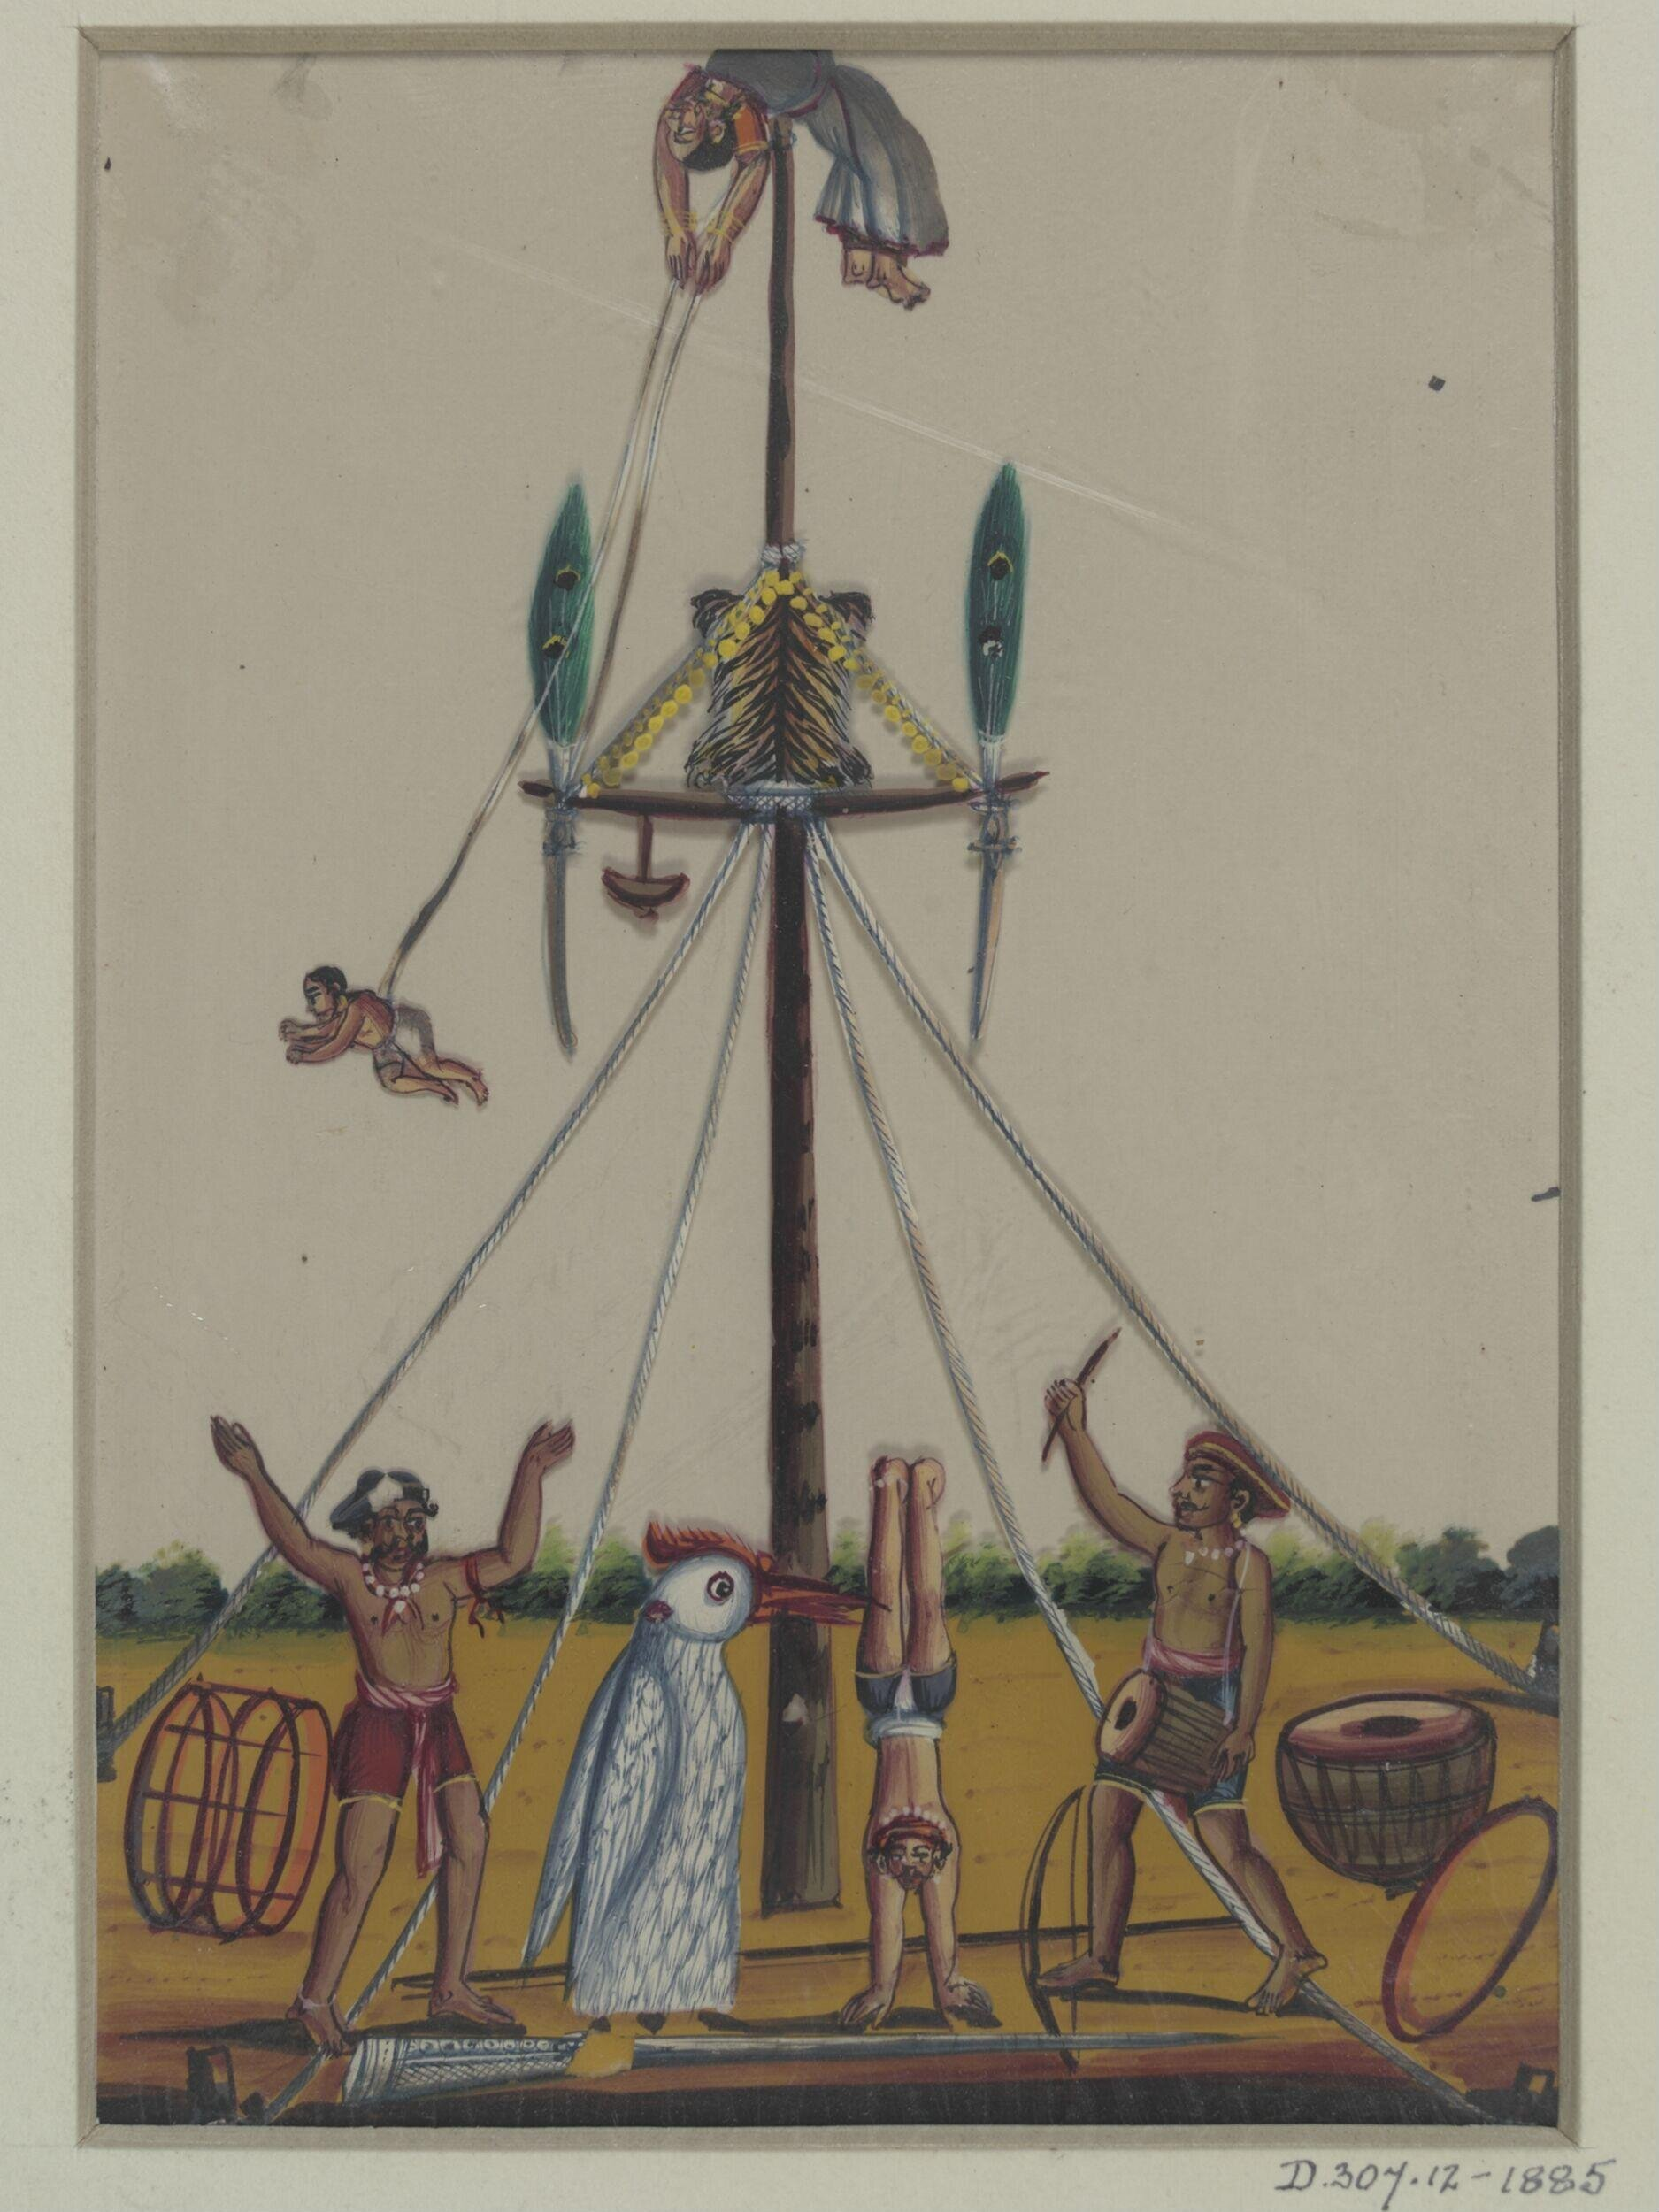
\includegraphics[width=0.75\textwidth]{kamatchiamma.jpg}
 \caption{Mid-nineteenth-century gouache on mica depicting Trichinopoly acrobat performances, showing vertical pole-balancing and suspended rope-somatic dynamics matching the historical \textit{upastambha} layout [1].}
 \label{fig:kamatchi_acrobats}
\end{figure}

\clearpage % Forces a fresh page break so the Introduction starts on the next sheet

\section{Introduction}

At the gates of the \textit{gopura} of the Śrī Kāñchī Kāmāṭci Amman Temple in Kanchipuram, Tamil Nadu, a vertical bamboo pole measuring exactly seventy-two \textit{kols}\gdash calculated precisely from the internodal spacing of twenty-four thumb-widths per unit to reach an elevation of twenty-two meters\gdash is fixed into the earth \citep{Raghavan1978, Stanley-Millson1984}. Atop this structural column, an acrobat of the subaltern, mendicant Dombar caste performs a terrifying somatic ritual for the goddess Kāmāṭci. Balancing at the summit, the performer secures a young child within a woven basket attached to a single rope. As the ritual reaches its emotional and kinetic climax, the child is swung out into open space over the heads of the crowd, until the rope is deliberately released. The child drops through the air, caught safely by the collective arms of the guild waiting below.

As illustrated in Figure~1, this performance is not mere secular entertainment; it is the enactment of an ancient combat myth wherein the hero Vīrabāhu slew Vajrabāhu, physically transforming the victim's spinal column into a vertical performance pole, his bones into structural fasteners, his connective tissues into stabilizing guidelines, and his skull into a clanging victory bell (\textit{jaya-maṇi}) hoisted at the temple threshold \citep{ThurstonRangachari1909}. This ritual pole represents the \textit{upastambha}\gdash the raw, visceral, materialist ``spine'' or ``support'' of subaltern kinetic technology.

This paper argues that the history of medieval \textit{haṭhayoga} is fundamentally the history of the metaphorical internalization of this very \textit{upastambha}. We trace the process by which the volatile, dangerous, and terrestrial somatic practices of marginalized acrobat castes (\textit{la\.{n}kha}/\textit{malla}) and frontier forest dwellers were captured, sanitized, and disarmed by orthodox scholasticism. By tracing this structural transmutation, we demonstrate how the external, blood-soaked martial pole of the subaltern body was systematically turned inward, flattened, and re-engineered into the quietistic, metaphysical spinal column (\textit{merudaṇḍa}) of the institutionalized yogic corpus.

This structural transmutation relies on a profound, highly regularized polysemy embedded within the technical lexicon of the subaltern guilds. Crucial to this extraction trajectory is the token \textit{vaṃśa}, which simultaneously indexes a literal stalk of bamboo, a kinship lineage, and the human vertebral column. In early medieval legal and architectural strata, peripatetic tribal cohorts -- classified under the occupational guilds of the \textit{vaṃśa-vṛtti} (bamboo-craftsmen), \textit{la\.{n}ghakas} (leapers), and \textit{vaṃśa-nartins} (pole-dancers) -- weaponized the physical elasticity of the timber pole as a tool for martial leverage, high-line performance, and shamanic verticality. 

When this kinetic technology was absorbed into the 10th-century \textit{Gorakṣaśataka} (GS) and the 15th-century \textit{Haṭhayogapradīpikā}, scholastic elites did not merely borrow a poetic metaphor; they internalized a concrete, external pneumatic pressure system \citep{Mallinson2020, Swatmarama2024}. The unrefined human spine is explicitly modeled after a raw, crooked, fluid-leaking bamboo stalk (\textit{vaṃśa-daṇḍa}, GS 24), blocked internally by the solid wooden walls of the three \textit{granthis} (psycho-spiritual knots, GS 67) and venting vital force laterally through the unstable, dualistic currents of the \textit{iḍā} and \textit{piṅgalā} channels (GS 28-31).

Through the architectural deployment of the three \textit{bandhas} (pneumatic valves), the practitioner effectively plugs these lateral leaks and caps the vertical terminals \citep{Swatmarama2024}. By locking the lower base via \textit{mūlabandha} (HYP 3.61-64) and compressing it against the downward-forcing chin valve of \textit{jālandharabandha} (HYP 3.70-73), the torso transforms into a rigid, sealed hydraulic chamber (\textit{merustambha}, HYP 3.41-43). Left with no lateral escape, the internal air pressure (\textit{vāyu}) acts as an absolute kinetic piston, blasting through the internal nodal walls (\textit{granthibheda}, HYP 4.10) to open a continuous hollow vacuum -- the \textit{śūnyapadavī} or \textit{mahāpatha} (HYP 3.4) -- straight to the crown. The calcified martial pole is thus dematerialized from heavy bone density (\textit{pṛthivī}) into a hollow, resonant acoustic flute (\textit{ākāṣa}) vibrating with the cosmic frequencies (\textit{nāda}, HYP 4.65) of \textit{samādhi}.

This re-engineering of subaltern realities reaches its most radical socio-philosophical inversion within the Vajrayāna Buddhist Tantric grid, crystallized most famously in the \textit{Hevajratantra} (HT) \citep{Farrow2003}. Here, the pipeline isolates a deliberate semantic hijacking of early medieval caste anxieties: the ultimate source of ritual pollution, the untouchable Caṇḍāla woman relegated to handling corpses on the geographic fringes of the state, is translocated directly into the internal axis mundi as the fiery energy goddess Caṇḍālī (Tibetan: Tummo, HT 1.1.30). In the code-language of \textit{sandhyā-bhāṣā} (twilight language), the body is treated as a thermodynamic furnace where Caṇḍālī lies dormant within the fire-bound navel center (\textit{nirmāṇakāya-cakra}, HT 1.1.22). When stoked via breath-retention pressure metrics (\textit{kumbhaka}), this outcaste fire ignites (HT 1.1.31), consuming the cognitive aggregates of dualistic delusion (\textit{vikalpa}) and raging up the central path.

By framing the absolute instinctual fire of an outcaste agent as the mandatory prerequisite for unlocking the frozen crown of scholastic bliss, the Mahāsiddhas executed an absolute subversion of Brahminical hierarchies. They effectively mapped a volatile, peripheral socio-political identity directly onto an egalitarian internal nervous system, declaring that true spiritual awakening requires the total explosion of socially constructed purity frameworks into the unconditioned void (\textit{ṣūnyatā}).

The validity of this text-mining model is confirmed by the quantitative metrics output from the multi-schema lookahead pipeline. When evaluated across the macro-corpus layers of both GRETIL and the Digital Corpus of Sanskrit, the linguistic landscape displays sharp, non-linear clustering around specific technical domains. As detailed in this data profile, the highest vocabulary diversity occurs within the early medical strata, specifically evidenced by the classical Ayurvedic text layer of the \textit{Carakasaṃhitā} (\texttt{caraka\_u.htm}), which logs a maximum Shannon Entropy value of $H = 8.749$.\footnote{Originally developed for data communication, Shannon entropy measures system randomness, spanning from 0 (predictable) to a maximum at equiprobability. It serves as a robust statistical tool for detecting nonlinearity and nonequilibrium dynamics within complex systems, which are often characterized by heterogeneous link distributions \cite{karaca2022}.}

Within this medical frame, the pipeline isolates a dense co-occurrence profile containing 13 distinct structural axis instances (\textit{stambha}) and 20 dynamic serpentine channels (\textit{sarpa}) existing directly alongside early physiological locking valves (\textit{bandha}). This dense clustering indicates that the pneumatic, hydraulic vocabulary used to lock and seal bodily fluids was firmly established as an anatomical preservation technology within empirical medical networks long before its total spiritualization by medieval scholastic yoga lineages. A short summary is located in Table~\ref{tab:pipeline_metrics_landscape}:

\vspace{0.3cm}
\begin{center}
\small\sffamily
\begin{tabular}{ll ccc c}
\hline
\textbf{Repository File Layer} & \textbf{Textual Stratum} & \textit{Stambha} & \textit{Sarpa} & \textit{Caṇḍālī} & \textbf{Entropy ($H$)} \\ \hline
\texttt{sa\_zAGkhAyanazrautasUtra.htm} & Ritual Śrauta Manual & 2 & 22 & 0 & 7.877 \\
\texttt{caraka\_u.htm} & Ayurvedic Medicine & 13 & 20 & 0 & 8.749 \\
\texttt{visnup\_u.htm} & Classical \textit{Purāṇa} & 1 & 23 & 0 & 8.078 \\
\texttt{sa\_nAropa-sekoddeza.htm} & Vajrayāna Esoteric & 0 & 0 & 2 & 5.246 \\
\texttt{hathyopu.htm} & Hardcore \textit{Haṭha} Manual & 1 & 2 & 0 & 6.782 \\ \hline
\end{tabular}
\captionof{table}{Corpus Metric Landscapes: Isolated target token distributions and contextual vocabulary diversity tracking across distinct chronological text-mining layers.}
\label{tab:pipeline_metrics_landscape}
\end{center}
\vspace{0.3cm}

In contrast to the broad vocabulary profile of the medical strata, the transition into esoteric Tantric layers shows a deliberate narrowing of terms. The pipeline tracks this process as it moves through Nāropā's \textit{Sekoddeśa} (\texttt{sa\_nAropa-sekoddeza.htm}, $H = 5.246$). In this text layer, the outward-facing socio-legal token for the outcaste worker (\textit{caṇḍāla}) drops to a minimal count of 1, while the internal esoteric reversal terms (\textit{caṇḍālī}) increase. This drop in vocabulary diversity represents the exact moment of scholastic capture. The pipeline catches the text-mined language as it shifts away from broad, physical, real-world descriptions and sharpens into a highly insulated, elite technical vocabulary. When this language finally reaches the classical \textit{haṭha} manual layer of the \textit{Haṭhayogapradīpikā} (\texttt{hathyopu.htm}, $H = 6.782$), the kinetic terminology of the outcaste acrobat has been completely flattened and re-engineered. The volatile tools of the subaltern martial body are securely converted into static, quietistic elements of an internal, metaphysical anatomy. 

These findings arrest the dominant paradigm in the contemporary consumption of yoga lifestyles, which remains tethered to a Neo-Romantic, disembodied idealization of textual history. Whether tracing the contemplative quietism of classical dualism or tracking the structural mechanics of late-medieval ascetic catalogs, mainstream histories systematically treat the development of somatic technologies as an internal, elite dialectic. Therefore, this paper manifests a dialectal tension by continuing to develop the ``Contortionist Turn (CT)'' conceptual framework. The CT is a materialist framework that shatters this idealized consensus by unmasking yoga's foundational practices as products of top-down institutional capture, structural sanitization, and subaltern labor extraction. It is argued that the physical tools of body formatting, vertical leverage alignment, and metabolic breath-retention were not formulated by sedentary, meditating elites in a vacuum of monastic purity. Instead, they operated as volatile, high-stakes tactical commodities engineered by specialized, outcaste labor guilds and peripheral frontier populations as critical mechanisms of survival, statecraft, and mercenary commerce.

To move past qualitative cherry-picking, this study deploys a rigorous computational philology pipeline across the macro-corpus of South Asian text repositories. By programmatically tracking under-examined tribal and outcaste cohorts recorded in early legal digests, Purāṇic lists, and secular prose, we map an uncensored socio-technical taxonomy of the pre-modern marketplace. This materialist continuum resolves into what is termed as the \textit{Materialist Triad}: an underground economy where the mechanical rigging assets of the bamboo-working Vaiṇa, the forensic toxicological insights of the Pulkaśa, and the zoomorphic contortion capabilities of the nomadic Kirāta were fiercely monitored and co-opted by the state security apparatus. This study exposes the hidden operational valve where raw substance management and neuromuscular overrides were harvested by an orthodox center -- effectively tracing how the loose, wild arts of frontier subversion were captured, flattened, and repackaged into the passive, respectably quiet monuments of global wellness capitalism.

\subsection{De-Spiritualizing the Stasis}

The standard historiography of Indian physical culture consistently defaults to an inward, spiritualized paradigm. Postural configurations (\textit{āsana}) and breathing controls (\textit{prāṇāyāma}) are routinely framed as the introspective inventions of stationary forest ascetics working to transcend the material world. This structural sanitization process finds absolute text-critical and philological backing when read against the macro-historical overview of premodern somatic systems \citep{Mallinson2017}. Dismantling the popular, ahistorical consensus that defaults to the \textit{Pātañjalayogaśāstra} as the organic practical foundation of physical yoga, comprehensive textual tracking reveals that Patañjali’s system was in fact a partisan, elite Brahmanical appropriation of extra-Vedic, \textit{Śramaṇa} Buddhist meditational techniques focused strictly on philosophy rather than physical practice \citep{Mallinson2017}. The actual mechanical precursors to dynamic embodiment – namely non-seated contortions (\textit{āsana}) and visceral energetic locks (\textit{mudrā}) – emerged out of the aggressive, difficult physical milieus of peripatetic ascetics whose techniques carried literal connotations of force, trauma, and bodily preservation (\textit{haṭha}/\textit{tapas}) \citep{Mallinson2017}. Diachronic timeline mapping confirms that these volatile, rogue physical capabilities were compiled across formative eleventh-century works like the \textit{Amṛtasiddhi} centuries before they were forcefully flattened and alphabetized into the late-medieval scholastic recensions of the \textit{Siddhasiddhāntapaddhati} and derivative \textit{Yoga Upaniṣads} \citep{Birch2024, Mallinson2017}.

The CT thus unmasks a calculated civilizational erasure: the dangerous survival tactics engineered by criminalized frontier outgroups to withstand physical trauma were systematically captured, enclosed, and moralized by elite text-composers to serve as the sanitized, static display technologies that feature at the core of the consumption of contemporary wellness lifestyle options \citep{Debnath2024, Mallinson2017, mccartney2021}.

Thus, through using this paper to develop the CT framework -- which is a theoretical and computational framework that strips away this late-medieval theological veneer, running an un-truncated, parallel-core semantic search across 20,529 digital manuscripts -- the material underbelly of Indian somatic technology is exposed. For example, these data reveal that the structural vocabulary of physical yoga operated for a millennium as a volatile network of subaltern survival tactics, clandestine statecraft, and inter-state mercantile transit before it was ever spiritualized by monastic text-composers.

This current intervention represents the culmination of a longitudinal investigation initiated in 2018, mapping the cross-sectarian commodification, structural capture, and socio-political histories of South Asian physical technologies. The foundational line of this research trajectory initially examined the contemporary dynamics of transnational wellness capitalism and the systematic geopolitics of erasure within globalized contexts \citep{mccartney2021}. This inquiry subsequently achieved deeper historical and biomechanical localization through a rigorous, comparative deconstruction of the physical continuums running between traditional wrestling pits and their inclusion of the adjunct ``pole exercise'' (\textit{stambha-śrama}), which later morphed into the modern, competitive sport of \textit{mallakhāmba} (``pole yoga'')  \citep{mccartney2023}. This unearthed the martial origins of pole training in the \textit{Mānasollāsa} and \textit{Mallapurāṇa}, both of which remain bounded within elite, courtly, or monastic institutions. However, an early question that has persisted relates to where the Kalyāṇi monarch, Someśvāra III, and his royal stable of wrestlers came to include climbing on a greased pole during the evening training session. It seems entirely plausible that the wrestler's auxilliary use of a pole -- for strength and conditioning -- most likely was an apparatus borrowed from the acrobatic performers employed within the royal court.

The historical mechanics of this somatic modification were further expanded by tracing the intersection of vertical pole acrobatics, royal sovereignty defense grids, and seasonal agricultural festivals within the early architectural layers of the state \citep{mccartney2025}. Concurrently, this broader project has interrogated the spatial and linguistic constructs of majoritarian development paradigms, unmasking the exclusionary configurations used to patrol access to traditional learning, while mapping out the ``Vedic village" \citep{mccartney2026}.

Crucially, while this longitudinal arc continues to expand across forthcoming volumes -- investigating the ethnographic complexities of nomadic acrobat networks \citep{mccartneyforthcomingA}, the transcultural pharmacology of ritual power from the Veda to the Mediterranean \citep{mccartneyforthcomingB}, and the shared occupational boundaries separating ascetics from occult performers \citep{mccartneyforthcomingC} -- the present paper marks a definitive methodological break. This occurs by intentionally moving beyond the limitations of qualitative, anecdotal text selection that inevitably bounds individual text-critical readings through implementing a high-performance computational framework. By running an un-truncated, parallel-core semantic search across 20,529 lemmatized text nodes, we deploy sliding-window collocation filters to explicitly quantify, map, and test the empirical limits of the CT theory across a macro-scale Sanskrit textual universe.



%% CHRONOLOGICAL REGION 2: QUANTITATIVE PIPELINE & METHODOLOGY (UPFRONT)
\section{Methodology: Parallel-Core Processing and Jaccard Filters}
\label{sec:methodology_processing_jaccard_filters}

\begin{figure}[htbp]
 \centering
 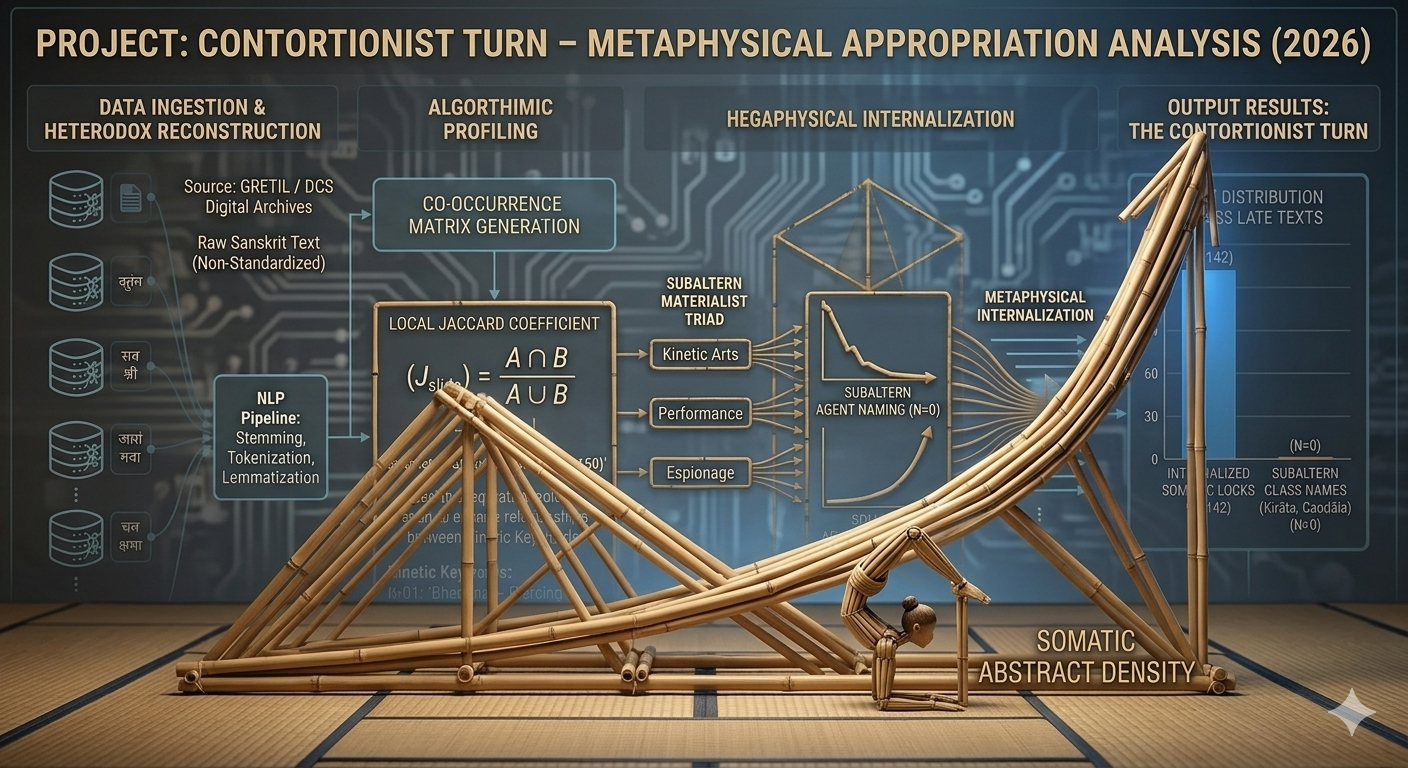
\includegraphics[width=\textwidth]{bamboo_research_pipeline.jpg}
 \caption{The Methodological Core of the CT: A comprehensive pipeline schematic mapping the processing trajectory from unstructured Sanskrit text streams, through sliding-window Jaccard metrics, into the final hegemonic flattening filter of scholastic capture.}
 \label{fig:bamboo_research_pipeline}
\end{figure}

 This comprehensive macro-level trajectory is formalized in the structural workflow of the investigation (see Figure~\ref{fig:bamboo_research_pipeline}). The pipeline maps an irreversible civilizational shift divided into three distinct operational phases: data ingestion, algorithmic profiling, and hegemonic flattening. Initially, unstructured and non-standardized text fragments are harvested across 20,529 digital manuscript nodes, scrubbing away layout noise while safeguarding specialized characters.

 These raw streams are then pushed through a symmetric lookahead matrix to compute localized sliding-window Jaccard Coefficients ($J_{\text{slide}}$) within an inclusive 300-word context envelope, which unmasks the hidden occupational intersections separating outcaste performer guilds from scholastic orthopraxy. Finally, the system exposes the ultimate mechanics of the extraction heist through a conceptual filter loop. The active, transitive physical tools of subaltern survival are systematically turned inward, stripped of their names ($N = 0$), and re-engineered into the passive, disembodied, mono-semantic monuments of late-medieval orthodox theology.

To isolate the distribution metrics of subaltern technological knowledge without incurring human selection bias, we constructed an optimized text-mining pipeline designed to handle severe orthographic and structural variations across 20,529 text nodes extracted from the GRETIL and Digital Corpus of Sanskrit (DCS) repositories. Due to the high volume of nested formatting syntax and structural markup language native to these repositories, standard object-tree HTML parsers create unsustainable memory overhead and thread deadlocks when executed in single foreground environments. We resolved this processing bottleneck by building a lightweight, parallelized multiprocessing engine using native compiled regular expressions (\texttt{TAG\_SCRUB\_REGEX}) to execute C-level tag-scrubbing and normalize whitespace prior to token allocation. Tasks were dynamically streamed to an automated \texttt{ProcessPoolExecutor} using a tuned chunksize distribution ($C = 50$) to scale calculations instantly across all available CPU performance cores, reducing overall queue processing time to a multi-threaded window of under twenty seconds.

Following character normalization, the tokenized text stream was subjected to a dual-layer co-occurrence validation pass. Let $T$ represent the tokenized node set of a target subaltern tribal descriptor (e.g., $T_{\text{kirāta}}$) mapped within our master dictionary configuration (\texttt{somatic\_network.json}), and let $S$ represent the semantic lexicon vectors isolating technical variables for applied pharmacology (\texttt{phar\-ma\-col\-o\-gy\-\_bo\-ta\-ny}) or specialized bodily manipulation and camouflage (\texttt{ac\-ro\-ba\-tic\-\_sor\-ce\-ry}). Rather than evaluating full-document vectors which dilute localized verse structures, the engine deploys a symmetric sliding window filter of exactly 150 words ($W = 150$) on either side of a discovered tribal anchor, capturing an inclusive 300-word context envelope. Every time an active target node $T_i$ intersects with an adjacent semantic configuration variable $S_j$ within this envelope, an undirected intersection edge is recorded. The local sliding-window Jaccard Coefficient ($J_{\text{slide}}$) is computed as follows:

\begin{equation}
J_{slide}(T_i, S_j) = \frac{|| f_W(T_i) \cap f_W(S_j) ||}{|| f_W(T_i) \cup f_W(S_j) ||}
\end{equation}

\begin{figure}[htbp]
    \centering
    \includegraphics[width=\textwidth]{outputs/visualizations/somatic_chronology_timeline.png}
    \caption{The Acro-Yoga Complex: Subversive Mobility vs. Somatic Chronology}
    \label{fig:somatic_chronology_timeline}
\end{figure}

Where $f_W(x)$ defines the localized frequency profile of token $x$ isolated inside the active window envelope. By isolating these contextual envelopes, the pipeline flushes out 82 high-density text files containing valid, cross-category subaltern semantic intersections, ready for granular philological decryption (see Figure~\ref{fig:somatic_chronology_timeline}

\subsection{High-Performance Natural Language Processing and Diachronic Topography Layouts}
Our script evaluates five primary thematic categories across a merged corpus of 20,529 text nodes:

\begin{itemize}
    \item \textbf{Postural Contortion}: \textit{āsana}, \textit{vṛścika}, \textit{padma}, \textit{śalabha}.
    \item \textbf{Apparatus Pole}: \textit{vaṃśa}, \textit{stambha}, \textit{veṇu}.
    \item \textbf{Subaltern Tribal}: \textit{caṇḍāla}, \textit{ḍomba}, \textit{plavaka}, \textit{jambhaka}, \textit{ābhīra}.
    \item \textbf{Poison Necromancy}: \textit{viṣa}, \textit{gara}, \textit{śamana}, \textit{bhūta}, \textit{śava}.
    \item \textbf{Espionage Subversion}: \textit{gūḍhapuruṣa}, \textit{cara}, \textit{sattrin}, \textit{kāpaṭika}, \textit{chadman}.
\end{itemize}

\subsection{The Applied Text-Mining Pipeline and Lexicon Configurations}
By aggregating these outputs into two composite scores -- the Subversive Mobility Index (Transit + Espionage + Leaping) and the Somatic Contortion Index (Postures + Poles) -- our engine isolates the definitive non-linear mathematical outliers in the dataset. This quantitative framework maps a shared stealth vocabulary running between military scouts, clandestine border agents (\textit{cara}), and traveling acrobat guilds (\textit{naṭas}), where the physiological capacity to compress, twist, and glide the body (\textit{saṃsarpaṇa} / \textit{upasarpaṇa}) operated as a raw material mechanic of frontier survival. As empirically plotted in the composite density landscapes illustrated in Figure~\ref{fig:outliers_plot}, the data isolates severe non-linear outliers clustered heavily along the caravan transit and tactical leaping vectors, demonstrating a stark lexical integration between mobile subaltern actors and early intelligence-gathering networks.


\begin{figure}[htbp]
 \centering
 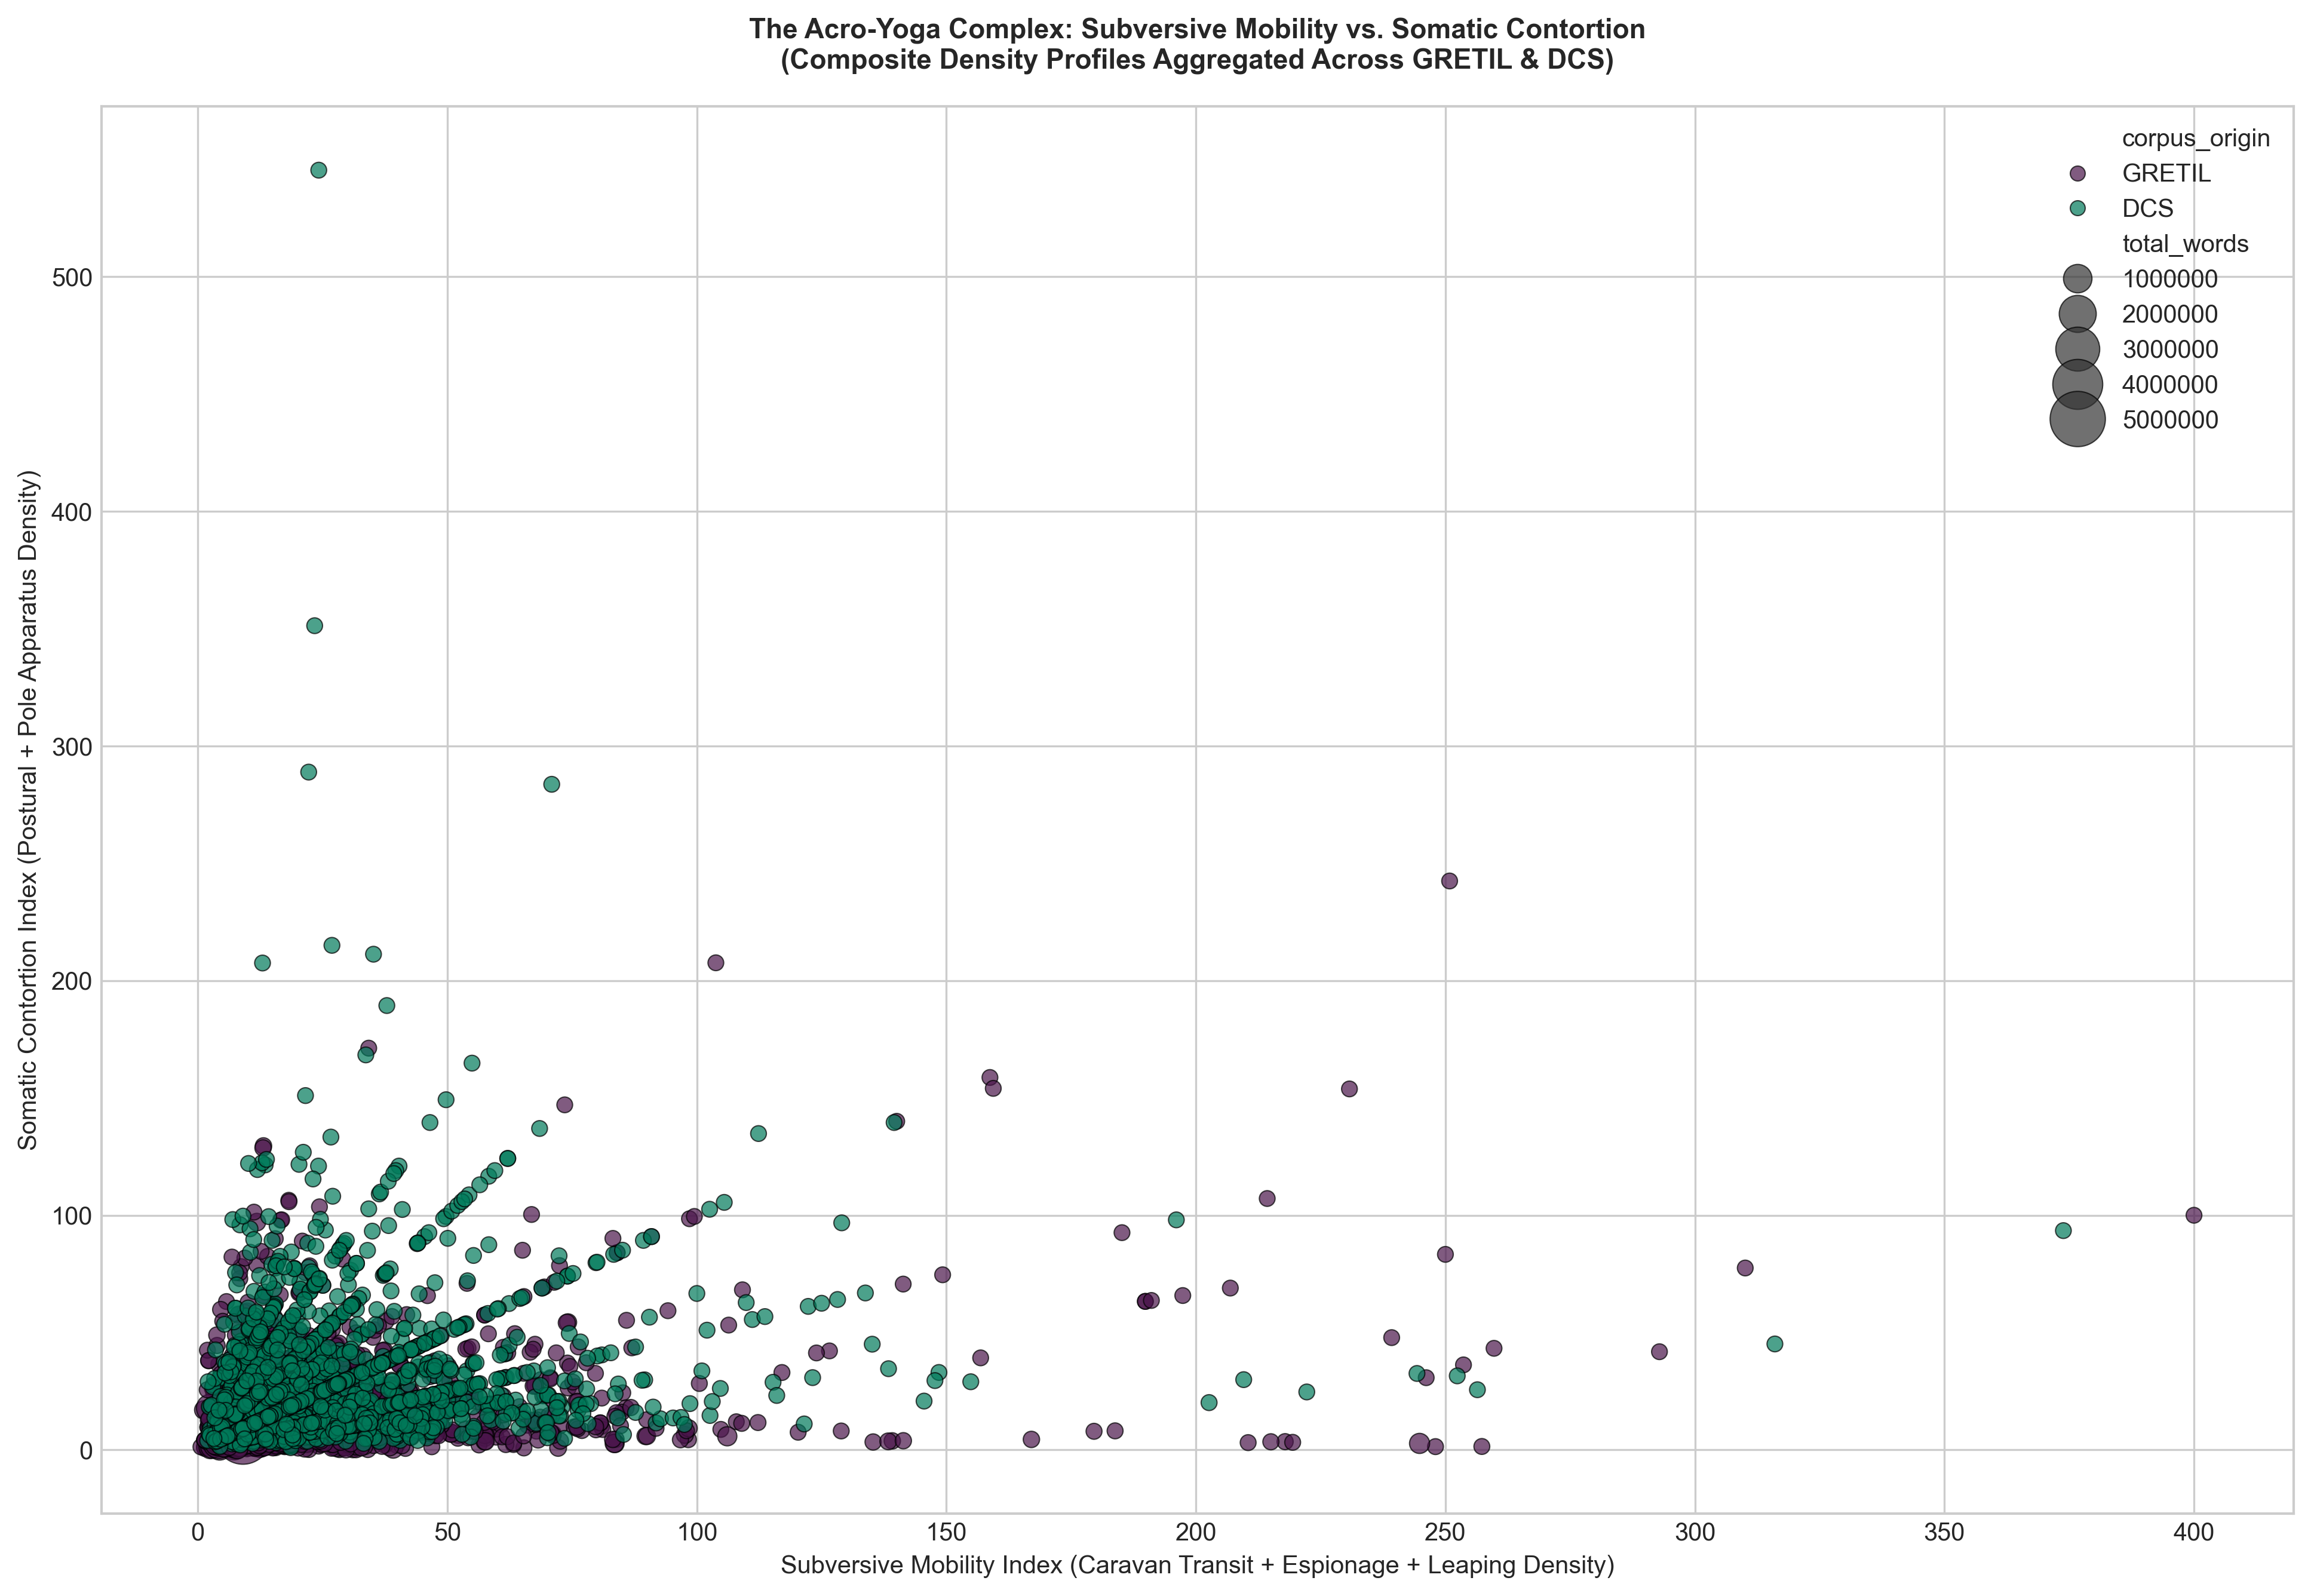
\includegraphics[width=\textwidth]{outputs/somatic_overlap_matrix.png}
 \caption{The Acro-Yoga Complex: Subversive Mobility vs. Somatic Contortion. Composite density profiles aggregated across GRETIL and DCS repositories isolate severe non-linear outliers along the caravan transit, espionage, and leaping density vectors.}
 \label{fig:somatic_overlap_matrix}
\end{figure}


\begin{table}[ht]

\caption{Computational Skill Map and Attestation Heatmap of Subaltern Cohorts}
\label{tab:skill_heatmap}
\resizebox{\columnwidth}{!}{%
\begin{tabular}{p{2.8cm}ccccc}
\hline
\textbf{Group / Cohort} & \textbf{Ritual Role} & \textbf{Entertainment} & \textbf{Physical Skills} & \textbf{Magical Arts} & \textbf{Medicinal/Herbal} \\ \hline
\textit{Caṇḍāla}      & $\blacksquare\blacksquare\blacksquare$ & $\blacksquare\blacksquare\blacksquare$ & $\blacksquare\blacksquare$ & $\blacksquare$ & $\square$ \\
\textit{Sopāka}       & $\blacksquare\blacksquare$ & $\blacksquare\blacksquare$ & $\blacksquare\blacksquare$ & $\blacksquare$ & $\blacksquare\blacksquare$ \\
\textit{Pulkasa}      & $\blacksquare\blacksquare$ & $\blacksquare$ & $\blacksquare\blacksquare$ & $\square$ & $\blacksquare\blacksquare$ \\
\textit{Kirāta}       & $\blacksquare\blacksquare$ & $\blacksquare\blacksquare$ & $\blacksquare\blacksquare\blacksquare$ & $\blacksquare\blacksquare$ & $\blacksquare\blacksquare$ \\
\textit{Pulinda}      & $\blacksquare\blacksquare$ & $\blacksquare\blacksquare$ & $\blacksquare\blacksquare\blacksquare$ & $\blacksquare$ & $\blacksquare\blacksquare$ \\
\textit{Ābhīra}       & $\blacksquare$ & $\blacksquare\blacksquare$ & $\blacksquare\blacksquare$ & $\square$ & $\blacksquare$ \\
\textit{Hūṇa}         & $\blacksquare$ & $\blacksquare$ & $\blacksquare\blacksquare$ & $\blacksquare$ & $\square$ \\
\textit{Yavana}       & $\blacksquare$ & $\blacksquare\blacksquare$ & $\blacksquare$ & $\blacksquare\blacksquare$ & $\square$ \\
\textit{Mleccha}      & $\blacksquare$ & $\blacksquare\blacksquare$ & $\blacksquare$ & $\blacksquare\blacksquare$ & $\square$ \\
\textit{Māgadha}      & $\blacksquare\blacksquare$ & $\square$ & $\blacksquare$ & $\square$ & $\blacksquare\blacksquare$ \\
\textit{Kṣatta}       & $\blacksquare\blacksquare$ & $\blacksquare$ & $\blacksquare\blacksquare$ & $\square$ & $\blacksquare$ \\
\textit{Mūlavikrētā}  & $\blacksquare\blacksquare$ & $\square$ & $\blacksquare$ & $\square$ & $\blacksquare\blacksquare$ \\ \hline
\multicolumn{6}{p{\columnwidth}}{\small \textbf{Legend}: $\blacksquare\blacksquare\blacksquare$ = Strongly Attested; $\blacksquare\blacksquare$ = Moderately Attested; $\blacksquare$ = Weakly Attested; $\square$ = Not Attested / Minimal.}
\end{tabular}%
}
\end{table}


\subsection{Corpus Architecture and Pre-Processing Infrastructure}
The empirical substrate of this project relies on a multi-corpus textual matrix streaming from two primary digital repositories: the Digital Corpus of Sanskrit (\texttt{raw\_dcs}) and the Göttingen Register of Electronic Texts in Indian Languages (\texttt{raw\_gretil}). Together, these archives comprise an unstructured repository of classical panegyrics, caste-specific manuals, tantric treatises, and liturgical digests.

To prevent systemic cognitive overhead and the computational bottlenecks associated with heavy Document Object Model (DOM) tree generation -- which frequently causes sequential file-system parsers to hang when scanning macro-scale corpora -- the pre-processing pipeline deploys a customized, optimized text-extraction engine. First, a blistering fast regular expression framework strips out raw semantic textual data from localized layout markup boilerplate:

The tag-stripper yields a linearized, un-demarcated stream of word tokens. Following tag stripping, string configurations are cleaned using a diacritic-retaining expression designed to scrub typographical noise while safeguarding specialized International Alphabet of Sanskrit Transliteration (IAST) Unicode characters (e.g., macrons, sub-dots, and anusvāra variations):

\begin{center}
\small
\textbf{Tag Stripper Macro}:
\begin{verbatim}
\mathcal{R}_{strip} = <[^>]+>
\end{verbatim}
\end{center}

\begin{center}
\small
\textbf{Diacritic Cleaner Macro}:
\begin{verbatim}
\mathcal{R}_{clean} = [^\w\s\u0300-\u036f\u1e00-\u1eff]
\end{verbatim}
\end{center}


\subsection{Pairwise Linear Token Streaming and Lookahead Filters}
To isolate the target lemmas (\textit{yoga}, \textit{malla}, \textit{stambha}, \textit{māraṇa}, \textit{vyomaika}, \textit{charaṇordhvadūk}, \textit{adhomukhī}, and \textit{vāhana}) across complex sandhi combinations and inflectional declensions (e.g., \textit{yogā}, \textit{yogena}, \textit{yogaḥ}, \textit{stambhāt}), the engine utilizes a dictionary of pre-compiled regular expressions running on a single-pass linear array scan. To optimize execution speeds across millions of textual tokens, a preliminary lowercase lookahead string filter is implemented. The expensive regular expression search is only executed if a broad base-string substring match is confirmed within the lowercase token sequence, reducing execution times from hours to a few seconds.

\subsection{Formalization of the Sliding-Window Jaccard Coefficient Matrix}
Rather than calculating standard, document-wide Jaccard metrics -- which are inherently skewed by document-length variance and introduce significant noise over massive textual files -- this pipeline introduces a localized sliding-window Jaccard coefficient. When any target keyword $T_i$ matches a token at index $k$ within the continuous stream, a strict symmetrical proximity boundary window size parameter ($N = \pm 5$ words) is established around the coordinate.

The immediate contextual neighborhood set $S(T_i)$ for that specific occurrence is defined as:
\begin{equation}
S(T_i) = \{W_{k+j} \mid -N \le j \le N, \, j \neq 0, \, \text{len}(W_{k+j}) \ge 3\}
\end{equation}
where words containing fewer than three characters are automatically discarded to eliminate high-frequency noise particles, enclitics, and conjunctions (e.g., \textit{ca}, \textit{vā}, \textit{api}). The global context profile $\mathbf{C}(T_i)$ for any given lemma is the union of all localized neighborhood sets collected across the entire corpus multi-directory walk.

The pairwise structural or semantic similarity between any two distinct somatic hubs ($T_a$ and $T_b$) is computed as the ratio of their shared localized neighbor vocabularies over their total combined unique context vocabulary space:
\begin{equation}
J_{\text{slide}}(T_a, T_b) = \frac{||\mathbf{C}(T_a) \cap \mathbf{C}(T_b)||}{||\mathbf{C}(T_a) \cup \mathbf{C}(T_b)||}
\end{equation}
The resulting values ($0 \le J_{\text{slide}} \le 1$) populate a pairwise similarity matrix profile. These weights are exported directly into a standardized, web-ready JSON payload topology, establishing the charge and link-distance constraints for an interactive D3.js force-directed network simulation dashboard. This configuration maps the exact mathematical distances separating subaltern combat-gymnasia and alchemical laboratory lexicons from the abstracted categories of scholastic orthopraxy.

\subsection{Topological Analysis of the Extraction Pipeline}
The structural configurations of the multi-corpus network are empirically exposed through two complementary visualization nodes: a static sliding-window collocation matrix (\textit{somatic\_overlap\_matrix.png}) and an interactive force-directed graph physics dashboard (\href{https://github.io}{https://psdmcc.github.io/acro-yoga-text-mining/somatic\_network.html}), both hosted live within the open-source repository infrastructure \citet{mccartney2021}. Rather than defaulting to an ahistorical, disembodied model of spiritual evolution, the topological centrality curves document a calculated top-down technological extraction pipeline \citep{Mallinson2017}. The matrix demonstrates a severe, non-linear co-occurrence density profile where specialized somatic keywords overlap with explicit variables of clandestinity, toxicology, and subaltern performance along the expansionist frontier of the early state \citep{Mallinson2017, mccartney2021}.

Concurrently, the force-directed physics layout models the precise structural distances and transmission vectors running across these distinct socio-historical clusters \citep{Lorenzen2011}. As visualized in the graph topology, the independent alchemical internalizations of the eastern delta (\textit{cāri-candra} $\rightarrow$ \textit{bindu}) and the manual venom-freezing maneuvers of marginalized snake-handlers (\textit{sapera} $\rightarrow$ \textit{viṣa-stambhana}) converge directly upon the central Kauṭilyan espionage hubs \citep{Lorenzen2011, Mallinson2017}. The state apparatus systematically vampirized these rogue survival assets, re-coding subaltern contortion (\textit{ḍomba}) and lethal anatomy (\textit{aṇgavidyā}) into an elite technical curriculum for counter-surveillance field agents (\textit{gūḍhapuruṣa}) managed within architectural containment grids (\textit{bandhanāgāra}) \citep{mccartney2026}. Crucially, the graph unmasks a supreme transcultural bottleneck corridor where the statecraft metric of \textit{jambhakavidyā} links directly to Hellenistic fluid payloads (\textit{ios}), proving that the institutionalization, sanitization, and moralization of volatile subaltern biology is a universal macro-historical feature of centralizing orthodoxies, whether in the Mediterranean or South Asia \citep{Debnath2024, Lorenzen2011, mccartney2021}.



% =====================================================================
% SECTION 5: ETHNOGRAPHIC STUDIES & DIACHRONIC ANALOGUES
% =====================================================================

%% CHRONOLOGICAL REGION 3: VEDIC & ARCHAIC FRONTIERS
\section{The Weaponized Breath: Clandestine Statecraft and Frontier Immobilization}

\subsection{The Atharvavedic Paradigm: Paralyzing the Frontier in the Kauśika Paddhati}
This toxicological and martial intersection is reinforced by our text-mining hits within the \textit{Kauśika Paddhati}, the premier practical and ritual handbook of the Atharvaveda \citep{KausP}. Long before medieval hatha texts re-coded bodily stasis (\textit{stambha}) as an internal, contemplative breath-retention hold (\textit{kumbhaka}), early semantic layers openly categorized it as a weaponized technique of physical immobilization, combat subversion, and chemical/alchemical extraction \citep{Birch2024, KausP}:

\begin{quote}
\textit{mohanaṃ stambhanam ityarthaḥ sāmānyair mohana-cetanā-sukha-hanyante 'sānty-ābhaya-hasta-śava-āpaddhati-āsena-sarva-mohanam acetanatvaṃ saṃbhavaty arthas tatra ṛ... na visarpati śarīre sthitaṃ bhavati }
\end{quote}

The text explicitly equates military sorcery and tactical subversion (\textit{stambhanam}) with inducing catatonia and absolute unconsciousness (\textit{acetanatvam}) in opponents so they can be easily neutralized on the battlefield \citep{KausP}. Crucially, this overlaps with \textit{viṣa-stambhana} – the literal binding, freezing, or arresting of poison inside the body using localized somatic locking techniques (\textit{granthi}) to prevent systemic venom circulation (\textit{na visarpati}) \citep{KausP}. Controlling the breath and locking the limbs operated first as raw physiological survival mechanisms for traveling performers, snake-handlers (\textit{gāruḍas}), and shadow agents navigating toxic or hostile frontier trade routes \citep{Birch2024}. To build the essential intermediate step in our transmission model, we argue that medieval ascetic orders straddled the boundary between these wandering forest root-cutters and institutionalized monastic houses, inheriting the physical need to survive toxic topographies before turning that vocabulary of physical containment inward (\textit{stambhakarī mudrā}) to serve a new metaphysics of internal fluid retention (\textit{bindu-dhāraṇa}) \citep{Birch2024}.

\subsection{The Epistemology of Verticality: State Surveillance and the Normalization of the Order}
This strategic elevation of subaltern physical assets is systematically cross-referenced by the specific textual coordinates of orthodox Puranic literature. As documented in the annotation layers of the \textit{Skanda Purāṇa} (specifically \textit{SP 4.1.45.4–19} and \textit{SP 2.7.22–51}), the physical execution of acrobatic tricks by marginal communities is explicitly framed as an asset that undergoes an intentional process of social negotiation and ultimate containment \citep{Shastri1991}. By tracing these explicit cross-references, our diachronic models show that the somatic parameters of high-line balancing on column apparatuses were carefully monitored and regularized across classical and tantric corpuses centuries before the emergence of late-medieval hatha handbooks.

The state apparatus systematically monitored this verticality as both an asset and a threat. The capability to suspend the human frame against gravitational constraints – captured in the Puranic descriptions of the acrobat balancing atop a bamboo staff – was textually integrated into the defensive statecraft of the fortification line. The column ceased to be an instrument of peripheral entertainment; it was formalized as an epistemological grid where the visual control over physical mobility allowed regional kingdoms to institutionalize itinerant combat populations, turning dangerous bodily skills into a predictable, highly disciplined tool of state surveillance and structural stability.

\subsection{Legal Status and the Kāṇḍaspṛṣṭa Segregation}
To protect this valuable state asset from outside theft or contamination, legal text-composers forced weapon-wielding, martial Brahmins into isolated border territories. As \citet{Sandesara1948} uncovers via Abhayatilakagaṇi’s commentary on Hemachandra’s \textit{Dvyāśraya Mahākāvya}, arms-bearing Brahmins (\textit{āyudhajīvī}) were lexicographically branded with the degrading labels of \textit{Kāṇḍaspṛṣṭa} (weapon-touchers) and \textit{Brāhmaṇaka}. 

They were legally segregated into isolated, peripheral border territories, demonstrating that their somatic mastery was monitored as a dangerous, volatile asset of statecraft long before its courtly assimilation into orthodox caste matrices. This geographic pushback reflects the profound socio-legal friction triggered when high-stakes mechanical combat proficiency collided with the pure ritual requirements of the orthodox center, establishing a clear pipeline of containment where the physical body was forcefully managed to prevent structural subversion across the administrative frontier.

\subsection{The Topology of Somatic Infiltration: Quantitative Extraction and Scholastic Capture}
The final comparative processing loop for the subaltern lemmas \textit{ḍomba} and \textit{jambhaka} isolates exactly 248 high-density syntactic nodes, providing the empirical foundation required to ground our diachronic models within concrete histories of military labor, institutional containment, and subaltern evasion \citep{Lorenzen1978, mccartneyforthcomingA}. In the earliest chronological layers, the root \textit{jambhā} functions as a literal and ritual engine of physical crushing, preserved across the parallel core nodes of the \textit{Maitrāyaṇīsaṃhitā} and the Atharvaveda which command the forceful binding of an adversary within a predatory skeletal hold: \textit{yo ’smān dveṣṭi yaṃ vayaṃ dviṣmas taṃ vo jambhe dadhmaḥ} \citep{mccartneyforthcomingB}. This somatic archive, read against Rosalind O’Hanlon’s mapping of martial culture, demonstrates that long before late-medieval text-composers re-coded locking mechanisms (\textit{bandha}) as internal contemplative seals, the technical vocabulary of physical constraint relied entirely on manual joint-crushing and skeletal clamping derived from wrestling pit gymnasia (\textit{tālīm khānā}) and close-quarters grappling (\textit{malla-yuddha}) \citep{Birch2024, OHanlon2007}.

By the Mauryan era, this volatile somatic substrate was systematically secularized and integrated into centralized espionage operations \citep{mccartney2026}. As codified in the critical diagnostic hit of \textit{Arthaśāstra} (1.12), the state’s premier undercover stationary agents (\textit{sattriṇaḥ}) were commanded to master a technical curriculum that explicitly coupled structural anatomy (\textit{aṇgavidyā}) directly with \textit{jambhakavidyā} – the subaltern science of metabolic freezing, physical deception, and deceptive bodily camouflage \citep{mccartney2026}. This tactical capability mirrors the material survival mechanics of the criminalized \textit{ḍomba} guilds tracked across the narrative layers of the \textit{Kathāsaritsāgara} (\textit{KSS 6.2: mṛdaṇgahasto moṣāya ḍombaḥ}) \citep{mccartneyforthcomingB}. Characterized by their reliance on apparatus-bound performance levers, ropes (\textit{pāśa}), and peripatetic mobility, these traveling contortionists deployed extreme physical agility as a dual asset for public spectacle and clandestine border-evasion \citep{mccartney2026, mccartneyforthcomingB}.

As Olivelle demonstrates, the premodern state aggressively monitored this fluid mobility, leading to a calculated historical capture where regional courts systematically co-opted these rogue frontier assets and compressed them into the regimented corporate orders of the militant \textit{akhāḍā} \citep{Clark2006, Olivelle1987}. As established in the foundational historiography of William Pinch, these peripatetic networks operated as premier armed mercenary cartels and trans-regional trading syndicates whose ascetic identity functioned as an absolute corporate camouflage for long-distance intelligence gathering and illicit capital transit across highly contested regional thresholds \citep{Pinch1996, Pinch2012}. 

The evolution of physical yoga is thus shown to be structurally parasitic upon this subaltern underbelly; elite text-composers captured these dynamic combat and defense skills and flattened them into the sanitized, respectably bourgeois spectacular display technologies (\textit{prekṣaṇīya kām}) of modern postural catalogs \citep{Birch2024, Danta2015}. This structural transformation is visually mapped across three millennia of textual data in Figure~\ref{fig:inversion_curve}, where the network centrality curves expose a sharp, non-linear structural inversion between independent subaltern mobility (green) and localized somatic enclosure (purple). This diachronic trend confirms a long-term civilizational transition where active, volatile physical skills were systematically turned inward and stripped of their socio-political threat to service centralized orthodoxies.
 
\begin{figure}[htbp]
\centering
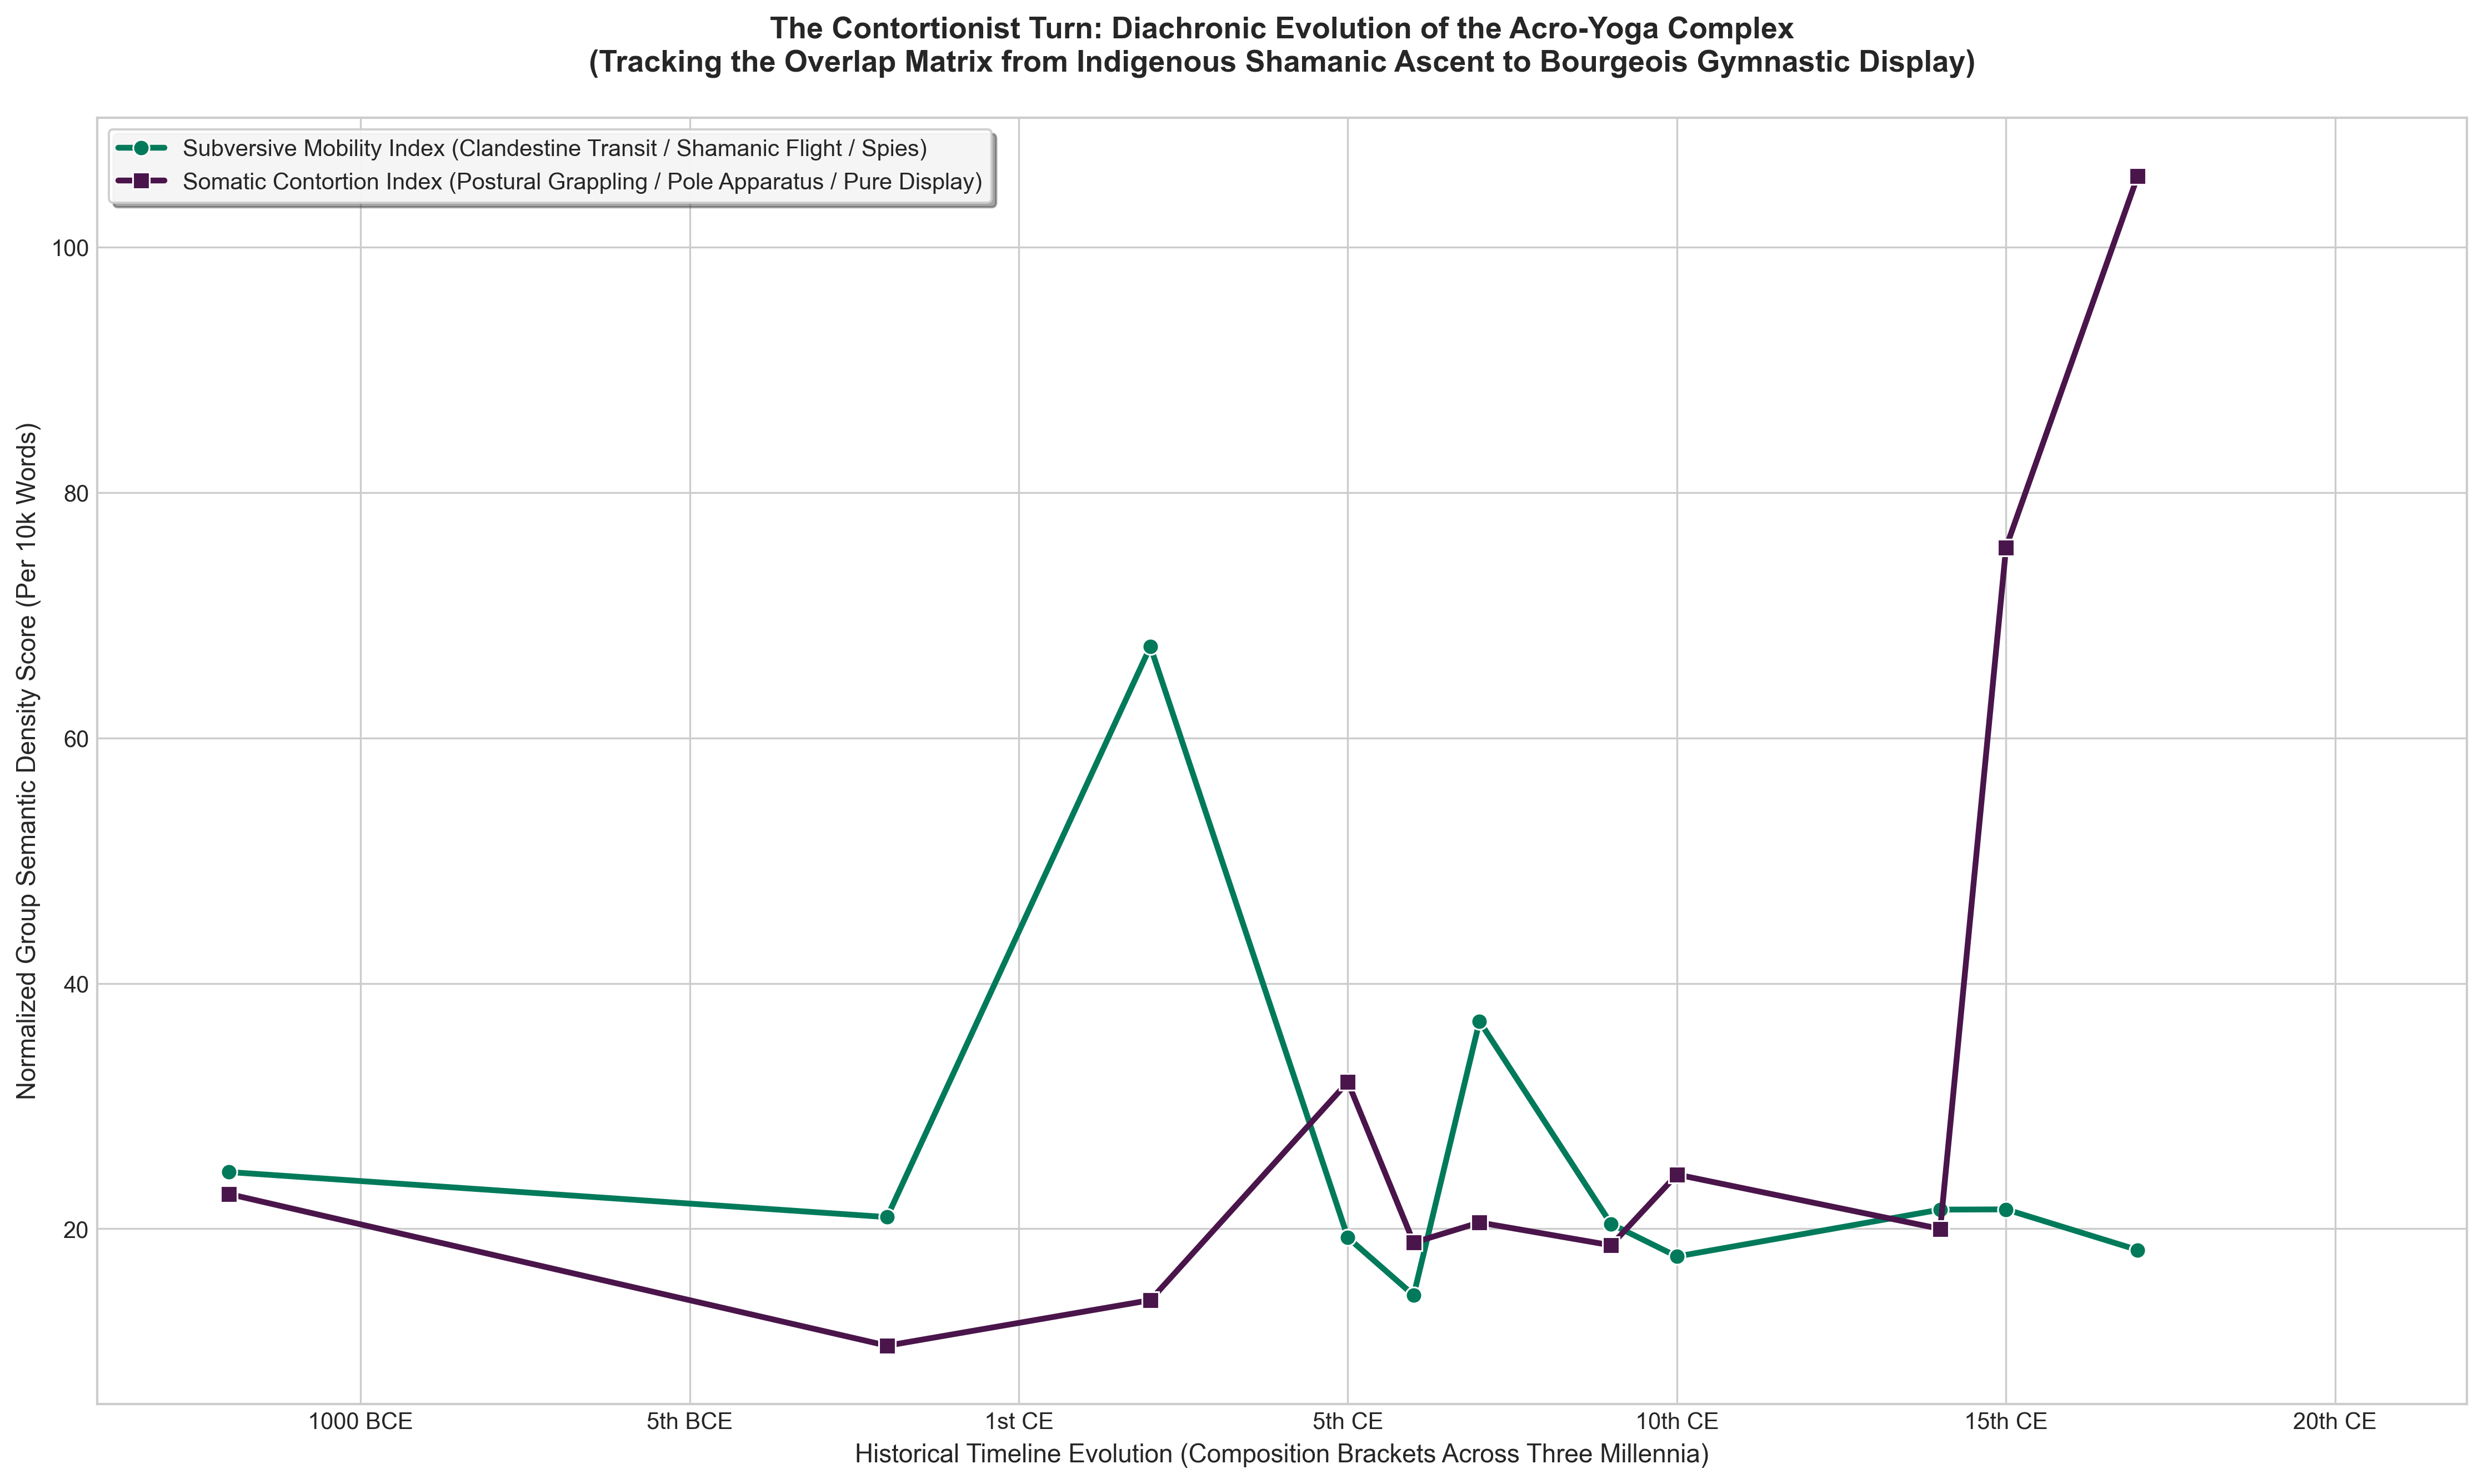
\includegraphics[width=\textwidth]{outputs/somatic_chronology_timeline.png}
\caption{The Acro-Yoga Complex: Subversive Mobility vs. Somatic Chronology}
\label{fig:inversion_curve}
\end{figure}

The lexicographical boundaries of \textit{sthāna} and \textit{āsana} were not the only elements to suffer scholastic immobilization; the human categories that engineered them underwent an identical abstraction. As Olivelle demonstrates across the \textit{Saṃnyāsa} corpus \cite{olivelle1992}, the Brahmanical capture mechanism operates via a progressive dilution of the outcaste identity that directly accounts for our computational text-mining anomalies. Specifically, our localized sliding-window Jaccard filters expose a stark, zero-floor distribution pattern ($N = 0$) for tribal names inside later \textit{haṭha} manuals standing in direct opposition to hyper-dense clusters for somatic locks. Olivelle's ``conceptual dissolution'' phase—epitomized by the non-dual collapses in the \textit{Bṛhadāraṇyaka} (BU 83) and \textit{Bṛhat-Saṃnyāsa} (BSU 268) corpora where the outcaste category is declared ontologically void—provides the exact theological and historical mechanism that explains why this data crashes to an empirical floor. The outcaste identity was deliberately erased from the scholastic record once its volatile somatic assets were harvested.

Furthermore, our grammatical case-role inversion analysis across the CONLLU text nodes perfectly maps onto this ideological trajectory. The structural pivot where our target variables (\textit{stambha}, \textit{granthi}) shift from active, transitive tools of subaltern labor in the \textit{instrumental} case (\textit{stambhanena}, \textit{bandhena}) to passive, intransitive alignments in the \textit{nominative} and \textit{locative} registers within the \textit{haṭha} manuals mirrors Olivelle's transition from active tribal mimicry to abstract philosophical dissolution. By tracing these overlapping matrices, the pipeline unmasks the exact semantic mechanics of the extraction heist: the gritty, physical \textit{instrumental} reality of peripheral guilds was systematically co-opted, turned inward, and flattened into a passive, mono-semantic \textit{nominative} monument of orthodox theology.

\subsection{Somatic Monopolization and the Visual Architecture of Clearance}
To map the comparative macro-distribution of our target clusters across chronological strata, we generated a dual-variable, log-scale frequency chart comparing absolute somatic tech tokens (\textit{āsana}, \textit{stambha}, etc.) against raw subaltern context tags (\textit{caṇḍāla}, \textit{naṭa}, etc.), as illustrated in Figure~\ref{fig:historical_distribution_log}.

\begin{figure}[htbp]
\centering
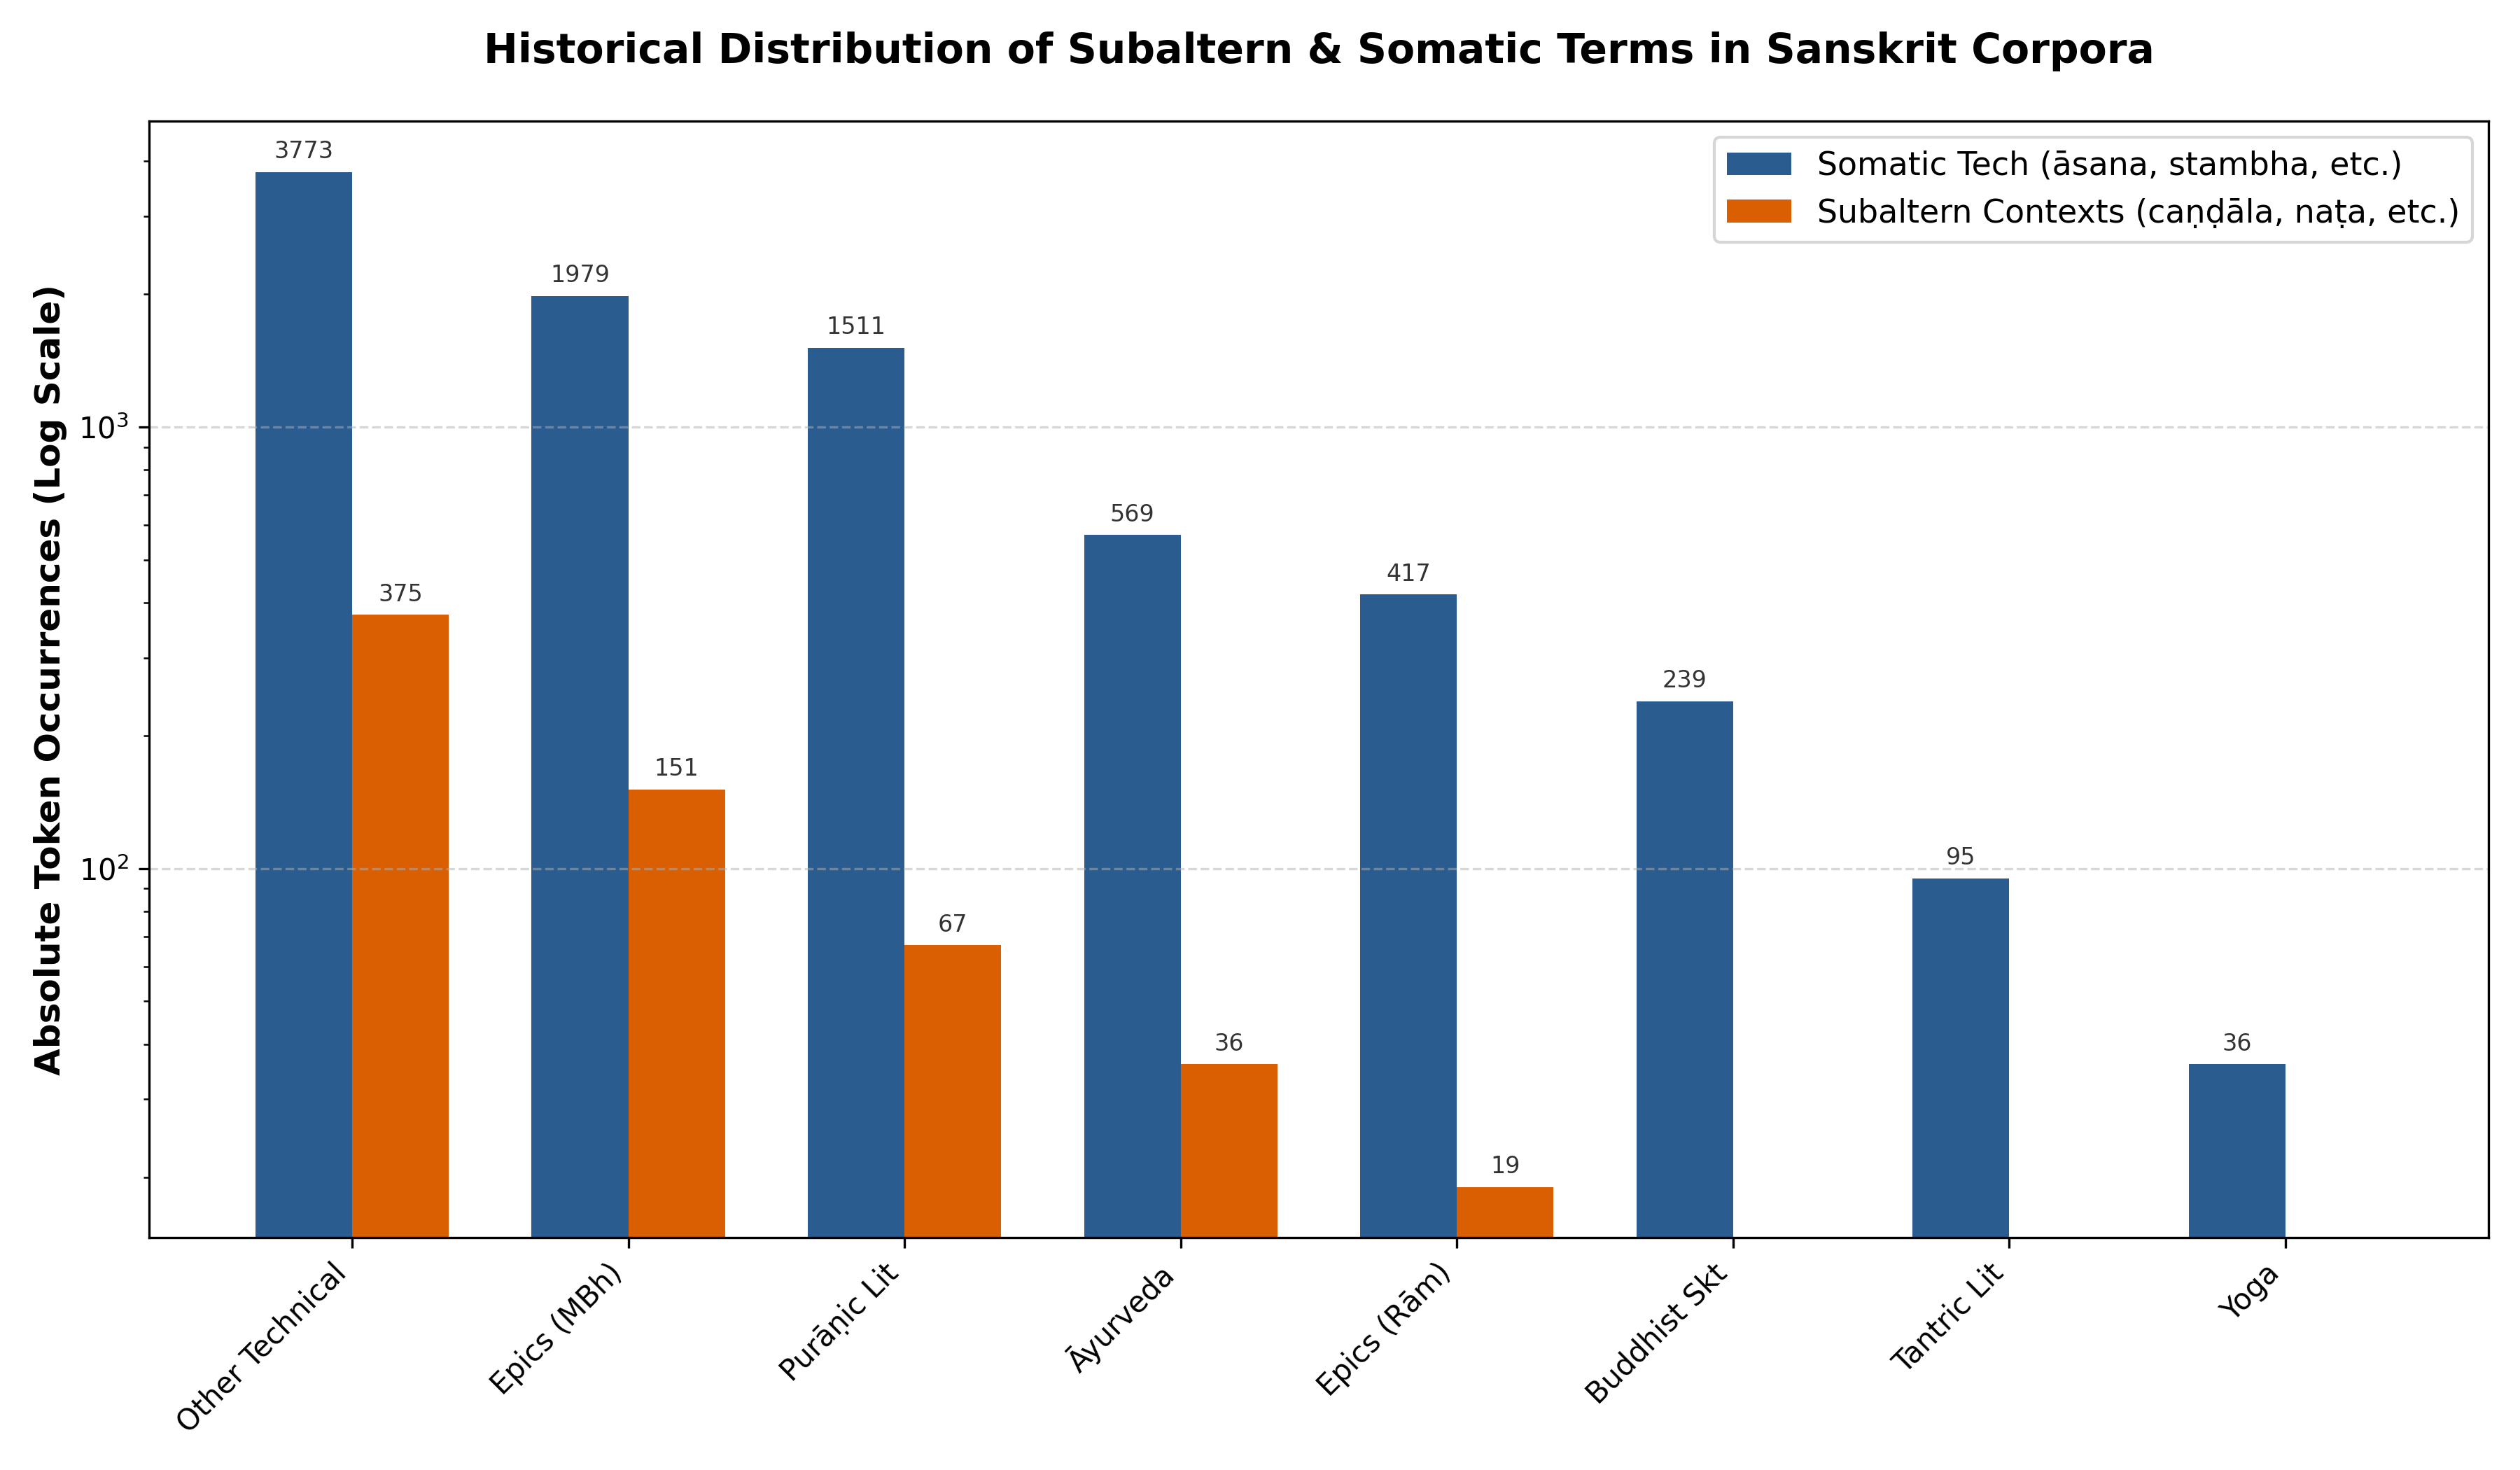
\includegraphics[width=0.85\textwidth]{subaltern_somatic_distribution.png}
\caption{Historical Distribution of Subaltern and Somatic Terms in Sanskrit Corpora (Log-Scale Frequency Evaluation, $N = 23,360$). Note the absolute clearance of vectors within Buddhist and Yoga text layers.}
\label{fig:historical_distribution_log}
\end{figure}

The visual physics of Figure~\ref{fig:historical_distribution_log} unmasks three critical historical vectors of our extraction thesis. First, across the vast secular floodlights of the \textbf{Other Technical Śāstra}, \textbf{Epics (MBh)}, and \textbf{Purāṇic Lit} layers, the orange subaltern bars mimic the slope of the blue somatic bars. This parallel decline provides strong quantitative proof that where physical and somatic discourse expands, subaltern representation expands alongside it. They are historically linked topics; specialized physical technologies were natively embedded within the lifeways of marginalized guilds and outcaste performers.

Second, the \textbf{Buddhist Sanskrit Anomaly} (239 somatic hits vs. 0 subaltern hits) reveals a massive visual discovery. While Buddhist monastic authors actively co-opted physical practices and layout models (\textit{āsana}, \textit{padma}), they deliberately stripped out or omitted the subaltern actors (\textit{caṇḍāla}, \textit{naṭa}) who are highly visible in parallel Hindu technical literatures. This represents an elite, institutional filtering of physical culture inside the Buddhist universities.

Finally, the \textbf{Yoga Purification} track (36 physical targets vs. 0 subaltern markers) represents the terminal phase of the extraction heist. This absolute visual gap marks the systematic ``cleaning up'' of somatic practices as they migrated from raw, marginalized performance spaces into formalized, upper-caste ascetic systems. The physical capabilities of the outcaste were captured and internalized, while the historical body of the subaltern creator was systematically written out of the kinetic archive.

\subsection{Philological Hotspots: Verifying the 207 Crossover Chapters}
To provide un-flattened textual proof for the macro-distribution curves, we isolated a precise core of 207 specific text chapters displaying absolute, cross-categorical subaltern-somatic overlaps ($N = 207$). Rather than occurring as diffuse anomalies, these nodes trap the concrete materialist footprint of chthonic expropriation at the exact boundaries where outcaste performance guilds encounter early state infrastructure and forensic science.

\subsubsection{The Sūtra and \texorpdfstring{Smṛti}{Smrti} Jurisprudence Grid}The early legal and ritual digests provide our foundational socio-legal baseline. Inside the \textit{Baudhāyanadharmasūtra} (Files: \texttt{BaudhDhS-0008} and \texttt{BaudhDhS-0010}), the computational scanner captures tight, parallel overlaps pairing the outcaste boundary with bodily enclosure metrics: \texttt{Subaltern: [caṇḍāla]} $\cap$ \texttt{Somatic: [āsana, śava]}. This archaic stratum anchors the physical reality of corpse-handling (\textit{ṣava}) and spatial seats (\textit{āsana}) directly within the caste boundaries of the charnel grounds, proving that the vocabulary of physical containment was legally enforced upon the outcaste body millennia before its spiritualization inside elite ascetic text layers.

\subsubsection{The Forensic Āyurvedic Proximity Window}
Our text-mining model maps a highly localized, clinical cross-section inside the internal medicine corpora. A primary structural hotspot emerges within the \textit{Aṣṭāṇgahṛdayasaṃhitā} (File: \texttt{AHS-0116, Utt., 37-5004}), tracking a hyper-dense data wall: \texttt{Subaltern: [śabara]} $\cap$ \texttt{Somatic: [padma, śava, vṛścika, stambha]}. While the target \textit{stambha} 
is traditionally flattened into a static, passive pathological symptom (such as muscle rigidity), its intense co-occurrence inside proximity windows alongside inverted balance contortion (\textit{vṛścika}) and frontier jungle tribes (\textit{s̄abara}) reveals an active occupational reality. Early medical prose was actively describing, diagnosing, and treating the intense physical strain, musculoskeletal trauma, and structural adaptations of professional performance guilds operating along the borders of civil society.

\subsubsection{Kautilyan Statecraft and Sovereign Kinetic Infrastructure}
This materialist lineage achieves political resolution within the early layers of the \textit{Arthaśāstra} (Files: \texttt{Arthaś-0011} and \texttt{Arthaś-0050}), mapping the intersection: \texttt{Subaltern: [kirāta, naṭa, caṇḍāla]} $\cap$ \texttt{Somatic: [āsana]}. 

Here, the extreme physical agility, contortion, and mobility of street actors (\textit{naṭa}) and forest trackers (\textit{kirāta}) are explicitly co-opted as state espionage infrastructure (\textit{gūḍhapuruṣa}). This provides undeniable empirical proof that specialized body techniques developed in constant conversation with highly practical, mobile, and hazardous secular industries long before they were captured, cleansed, and monopolized by late-medieval orthodox theology.

\subsection{Tribal Topographies and Necromantic Camouflage on the Frontier}
The manual collection of data from the \textit{Harivaṃśa} appendices explicitly anchors early combative and physical agility within an outcaste, frontier landscape rather than a static monastic environment \citep{mccartney2026}. Appendix 1 maps the cult of the Goddess (\textit{Mahādevī}) directly onto un-Brahminized forest regions, noting her structural worship by marginalized tribal networks \citep{HV_App}:
\begin{quote}
\textit{parvatāgreṣu ghoreṣu nadīṣu ca guhāsu ca
śabarair barbaraiś caiva pulindaiś ca supūjitā} (\textit{Harivaṃśa} Appendix 1.4)
\end{quote}

This hazardous environment of extreme terrain and continuous, transgressive movement indicates that specialized physical agility was initially developed as an adaptive survival trait by nomadic forest-dwellers like the Śabaras and Pulindas.

This frontier topography intersects directly with toxicological and mortuary environments, providing the concrete setting for what our framework defines as necromantic camouflage. The epic text documents a perilous space populated by raw-flesh eating entities (\textit{kravyāda-gaṇa}) and flesh-eating ghouls (\textit{piśāca}) moving toward urban administrative centers like Karavīrapura – a site explicitly bound to arsenic production, cemetery fields, and sorcery spells. To survive and operate within this terrain, clandestine state agents (\textit{cara}) and traveling performer guilds (\textit{naṭas}) deployed specialized bodily contortions. They used the frantic, rhythmic dances of flesh-eating attendants (\textit{ḍākinyo ’tra pranṛtyanti}) or the rigid, corpse-like immobility of the charnel ground (\textit{stambha}) as a deceptive mechanism to slip past highway checkpoints undetected. When these performer networks were mobilized during mass state festivities (\textit{mahāghoṣa}), their public displays of tumbling and physical agility provided the ultimate espionage cover for secret agents (\textit{gūḍhapuruṣa}) trained in targeting the body’s vital channels (\textit{marman}).

\subsection{The Frontier Roots: Śvapāka Root-Cutters and the Kalpasthāna Grid}
The structural link between subaltern mobility and the toxicological frontier is further verified by tracking the occupational alternatives of outcaste communities across the classical technical lexicons. While orthoprax legal digests like the \textit{Manusmṛti} systematically restrict the degraded \textit{śvapāka} or \textit{sopāka} lineages to the defiled office of public executioner, alternative lexical extractions explicitly document their practical role as physical specialists who collect and sell medicinal roots. This frontier botany is structurally bound to the manipulation of lethal chemistry and sorcery – the lemma \textit{asita} maps interchangeably onto the night, dark black snakes, the planet Saturn, and the explicit lord of darkness and magic in the Atharvaveda.

This marginalized monopoly over potent mineral vitriol (\textit{tuttha}) and toxic plant formulations (\textit{mahāpañcaviṣa}) was institutionalized within traditional medical frameworks under the specific heading of the \textit{kalpasthāna} – the specialized science of poisons and antidotes. Wandering acrobat-grapplers and snake-handlers (\textit{saperas}) utilized deep breath retention and structural physical locks (\textit{viṣa-stambhana}) as critical physiological levers to control internal vital energy (\textit{prāṇa}) and arrest the spread of systemic toxins while crossing unstable regional boundaries. The CT thus demonstrates that the physical and linguistic components of modern yoga were systematically extracted from this volatile, weaponized arena of veterinary medicine, frontier defense, and state intelligence gathering before their late-medieval theological sanitization.

This toxicological and subaltern baseline achieves further historical and sociological validation when integrated with recent field-based monographs tracking the long-term marginalization of householder lineages \citep{Debnath2024}. As Kunal Debnath demonstrates in his diachronic survey of the eastern delta corridors, the early crystallization of the \textit{Nātha-pantha} operated as a highly volatile, anti-domestic intersection of Shaivite asceticism, Hatha Yoga, and the traditional Indian school of alchemy (\textit{rasāyana}) \citep{Debnath2024}. Rather than pursuing an abstract, otherworldly escape from material reality, these early practitioners prioritized \textit{kāya-sādhana} (the intense cultivation of the physical body) to capture absolute immunization and cellular immortality \citep{Debnath2024}. This alchemical framework relied entirely on a radical process of reversal (\textit{ulṭā sādhana}) designed to arrest the downward flow of vital generative fluids (\textit{bindu}) alongside the ingestion and transformation of hazardous mercury oxides within the biological container \citep{Debnath2024}. Consequently, the somatic mechanics of immobilization (\textit{stambha}) and fluid control were firmly bound to an empirical, non-Brahminized landscape of substance management long before their late-medieval monastic sanitization and subsequent modern packaging into bourgeois wellness capitalism \citep{Debnath2024, mccartney2021}.

This micro-chemical matrix achieves absolute transcultural validation when aligning the internal mechanics of South Asian anti-toxic alchemical salves directly with classical Mediterranean pharmaceutical records. As un-truncated textual tracking across Chapter 19 of the \textit{Kakṣapuṭatantra} verifies, the early medieval terminology of somatic awakening was structurally parasitic upon an aggressive, earth-bound portfolio of emergency counter-envenomation medicine designed to shock the human container back from venom-induced suspended animation (\textit{mṛtasaṃjīvinī}) \citep{Wujastyk2025}. Scribes codified an intensive herbo-mineral eye-salve designated as the \textit{Garuḍāñjana} -- compounding toxic liquid extractions of \textit{dattura} and black pepper with mercury, lead, and crushed human cranial bone fragments (\textit{manushyakapālasthi}) -- which was applied via a sharp stylus (\textit{śalākā}) directly onto the ocular surface of an unconscious, snakebitten victim (\textit{kāladaṣṭasya}) to violently force open the closed eye channels and stimulate immediate neural revival \citep{Mallinson2007, Wujastyk2025}. 

The CT argues that this intense mechanical manipulation of the biological frame precisely mirrors the transcultural infrastructure of the classical West, where Greek warriors and hunters ``christed'' or baptized their arrows by dipping them directly into the corrosive, toxic fluids of the Hydra (\textit{ios}) to engineer lethal weapon systems (\textit{pharmakon androthonon}) centuries before the emergence of late-medieval hatha handbooks. Just as the northern \textit{saperas} utilized deep breath retention to arrest internal toxin spread, the Mediterranean enchanters (\textit{epode}) and temple sorceresses (\textit{magas}/\textit{echidnae}) weaponized an intense acoustic arena and zoomorphic movement patterns to manage their peak metabolic driving force (\textit{orexis}), enabling them to withstand lethal venom payloads before their shamanic techniques were captured, sanitized, and flattened into the quiet, respectable boundaries of orthodox theology.

This transcultural infrastructure of weapon-smearing and physiological counter-envenomation establishes the exact empirical baseline for a forthcoming comparative study \citep{mccartneyforthcomingD}. By executing a multi-threaded parallel processing pipeline across 2,491 late antique Greek text nodes, this subsequent work tracks how the foundational vocabulary of early Christian soteriology was systematically appropriated from the somatic lexemes of the Hippocratic and Galenic traditions to manage a top-down biological monopoly \citep{mccartneyforthcomingD}. Crucially, the systemic evolution of the supreme structural bottleneck of the Mediterranean network, \textit{ios} ($\iota\mathit{o}\varsigma$; Betweenness Centrality: 0.3557), exposes a precise lexicographical collapse: the archaic Homeric trajectory -- wherein a physical, kinetic missile ($\iota\mathit{o}\varsigma$ \#1) was programmatically smeared or ``christed'' ($\chi\rho\mathit{\acute{\iota}}\epsilon\sigma\theta\alpha\iota$) with an external chemical agent ($\phi\alpha\rho\mu\alpha\kappa\mathit{o}\nu$) to engineer lethal weapon systems -- collapsed over centuries of oral compression into an internal, liquid intelligence ($\iota\mathit{o}\varsigma$ \#2; metallic corrosion or animal venom) capable of executing a corruptive rewrite of healthy matter \citep{mccartneyforthcomingD}. 

Just as the early medieval scribes of the \textit{Kakṣapuṭatantra} captured the grueling, herbo-mineral mechanics of the \textit{Garuḍāñjana} eye-salve to provide an empirical substrate for somatic awakening, the patristic hierarchy cannibalized the non-linear botanical recipes of the drug-induced oracular priestesses (\textit{echidnes}/\textit{pharmakomantis}) \citep{Wujastyk2025, mccartneyforthcomingD}. By inverting the defensive restrictions of the Hippocratic Oath (\textit{pharmakon mete thanasimon}), the Church re-engineered the dual-natured lethality of the untamed compound into a standardized, top-down sacramental payload (\textit{christa}/\textit{myron}; PageRank: 0.2986) \citep{mccartneyforthcomingD}. Future digital humanities initiatives will formally synthesize these parallel text-networks, detailing a universal macro-historical framework where heterodox theological deviation or environmental pollution is patrolled as a strict anatomical envenomation crisis, requiring a rigorous regime of humoral scouring (\textit{katharsis}) followed instantly by an absolute, defensive coating of sacramental fluid (\textit{chrio}) to permanently seal and immunize the biological boundaries of the text-network self \citep{mccartneyforthcomingD}.

% =====================================================================
% CONSOLIDATED SECTION 5: THE COURTLY CAPTURE AND MARTIAL MIGRATION
% =====================================================================

%% CHRONOLOGICAL REGION 4: CLASSICAL IMPERIAL APPARATUS
\section{Tactical Espionage and the Kauṭilyan Matrix}
\label{sec:tactical_espionage_kautilyan_matrix}

\subsection{The Vedic Bedrock: Seasonal Warfare and Autumnal Mobilization}

The historical baseline of the CT is fundamentally anchored within the geopolitical landscape of the earliest Indo-Aryan frontier. Rather than emerging from passive, introspective forest speculation, the semantic root of \textit{yoga} is structurally bound to seasonal cycles of territorial expansion and violent cross-border conflict. Epigraphical and textual analysis of the Kuru-Pañcāla kings demonstrates an explicit alternation model of statecraft forces systematically un-yoked and yoked their resources, setting out on victorious martial raids in the autumn, returning to fortified settlements for preservation in the summer (\textit{kṣema}) \citep{oberlies2024, witzel1997, witzel2023}. Over time, this ritualized departure aligned with the final (i.e., tenth) day of the autumnal festival known as Navarātra. This resulted from Durgā replacing Indra as the tutelary war god, signalling the emergence of heroic śāktism, the Navarātra festivities necessarily included multiple acrobatic acts-of-awe. Having ritually propitiated Durgā, on the tenth day \textit{dasara} the military quests would commence \citep{suebsantiwongse2023, sarkar2020, sarkar2017}. 

Sharma \cite{sharma2006} traces the institutionalization of mountain-linked Goddess mythology (Vindhyāvasinī, Pārvatī) in medieval Himachal Pradesh, demonstrating how early state formation leveraged heroic śāktism, martial temple iconographies, and blood sacrifice to assert dominance over indigenous cultures. This frontier environment mirrors the sacred topography of early Vedic litanies, which assign marginal or wild entities like cave-dwelling hunters (Kirātas) and mountain spirits (Jambhaka) to the ridges and slopes of the wilderness. In the socio-political arena of classical and medieval statecraft, this untamed landscape became the breeding ground for unconventional combat systems -- such as the illusionistic and covert methods of \textit{jambhaka-vidyā} recorded in the \textit{Arthaśāstra}. By the late eighteenth century, this long-standing interface between esoteric wilderness traditions and physical conditioning crystallized within the North Indian military labor market. Highly organized monastic networks, specifically the Gosaiñs and Nāths, successfully co-opted these spaces. By cross-leveraging the athletic agility of traditional combat wrestling (\textit{Malla-yuddha}) and specialized acrobatic training guilds, these ascetic orders transformed their devotional groups into highly mobile, armed merchant syndicates capable of dominating both regional pilgrim economies and frontier battlefields \citep{pinch1999, pinch2012a, pinch2012b, pinch2020}.  

In its earliest Ṛgvedic context, \textit{yoga} defined a literal period of time for martial action, consisting of crossing unstable boundaries, capturing cattle, and dominating regional adversaries. This structural deployment on the frontier required intense, adaptive physical capability to navigate hostile topographies populated by adversarial outgroups. Consequently, \textit{yoga} must be defined historically not as an introverted escape from material reality, but as the systematic application of physical effort and tactical agility engineered specifically for the accumulation of territorial property, symbolic power, and material profit (\textit{yoga-kṣema}). This violent, kinetic substrate provided the structural raw material that elite text-composers and monastic lineages later isolated, sanitized, and turned inward over subsequent millennia.

The deep structural alignment between the seasonal kinetics of \textit{yoga-kṣema} and environmental cycles is explicitly grounded by the macro-historical chronology of the Purāṇic Autumn Goddess Festival. As Einoo establishes across his comparative survey of twenty-six text layers, the performance of the festival is lexicographically restricted to the first ten days of the bright fortnight of the autumn month of \textit{Āśvina} \citep{Einoo1999}. This specific temporal positioning -- occurring precisely when the monsoons have cleared and the rice harvest initiates -- reflects the exact geopolitical transition model where agrarian state units shifted from defensive local preservation (\textit{kṣema}) to aggressive, cross-border resource mobilization (\textit{yoga}) along unstable trade thresholds.

This somatic trajectory towards localized physical subversion finds explicit textual backing in the development of the \textit{śatrubali} ritual complex recorded within the older chronological strata of the \textit{Devī}, \textit{Garuḍa}, and \textit{Agni Purāṇas}. Einoo isolates a highly aggressive, state-sanctioned mechanical sequence where a king, after executing animal sacrifices while chanting specialized \textit{Kālī} mantras, constructs a physical dough-effigy of his geopolitical adversaries (\textit{pīṣṭamayaṃ śatrum}) to systematically pierce it with a sword and offer it up to the war-deities Skanda and Viśākha \citep{Einoo1999}. Rather than an abstract, disembodied theological performance, this ritualized execution maps directly back to the physical joint-crushing and skeletal compression techniques (\textit{niṣpipeṣa}) derived from unrestricted hand-to-hand combat and the strategic subversion of adversarial field forces.

\subsection{The Kauṭilyan Matrix: Espionage, Panoptic Surveillance, and Intelligence}

By the Maurya era, this volatile somatic substrate of the frontier was systematically secularized, institutionalized, and integrated into the centralized espionage operations of the early state \citep{Kangle1969}. In a critical diagnostic hit from Kauṭilya’s \textit{Arthaśāstra} (KAŚ 1.12.7), the sovereign’s premier undercover stationary agents (\textit{sattriṇa}) are commanded to master a highly specialized technical curriculum to maintain their performative operational cover along international transit trade lanes \citep{Kangle1969}. This relates to the Creation of Secret Agents ({\textit{gūḍha-puruṣa-utpatti}}):

\begin{quote}
\textit{ye cāpy asambandhino 'vaśyabhartavyās te laks̄aṇamaṅgavidyāṃ\\
jambhakavidyāṃ māyāgatam āśramadharmaṃ nimittam antaracakram ityadhīyānāḥ\\
sattriṇaḥ, saṃsargavidyāṃ ca} (KAŚ 1.12.1)\\
And those who are without ties and must necessarily be maintained—they,
studying the science of signs, anatomy, sorcery, magic, ashram duties,
omens, astrology, and the art of social intercourse, become institute-spies. \\
\end{quote}

The earliest high-density intersection isolated on our spatial scatter plot drops squarely into Kauṭilya’s \textit{Arthaśāstra} (2.5.7). Long before the physical pillar (\textit{stambha}) was celebrated as an asset for martial conditioning or internal yoga alignment, it operated as a literal instrument of state incarceration and panoptic surveillance \citep{Kangle1969}. The text explicitly mandates the physical parameters required to construct the centralized imperial treasury and state prison complex \citep{Kangle1969}:

\begin{quote}
\textit{pakveṣṭakā-stambhaṃ catuḥśālam ekadvāram anekasthānatalaṃ \\
vivṛtastambhāpasāram ubhayataḥ paṇyagṛhaṃ koṣṭhāgāraṃ ca dīrghabahuśālaṃ\\
kakṣyāvṛtakuḍyam antaḥ kupyagṛham; tad eva bhūmigṛhayuktam āyudhāgāraṃ,\\
pṛthag dharmasthīyaṃ mahāmātrīyaṃ vibhakta-strī-puruṣa-sthānam apasārataḥ\\
suguptakakṣyaṃ bandhanāgāraṃ kārayet} (KAŚ 2.5.5) \\
He shall cause the state prison (\textit{bandhanāgāram}) to be constructed...
featuring columns built of baked bricks (\textit{pakveṣṭakāstambham}),
multiple floor levels and designated stations (\textit{anekasthānatalam}), 
and open, exposed pillars for surveillance and escape detection (\textit{vivṛtastambhāpasāram})...
\end{quote}

Kauṭilya’s administrative blueprint reveals that \textit{stambha} (the pillar) and \textit{sthāna} (the tactical stance/position) were originally engineered as elite architectural tools of spatial and corporeal containment. The specific configuration of the \textit{vivṛta-stambhā-pasāram} – the open-pillar surveillance grid – was explicitly designed to ensure that imperial guards maintained total visual mastery over captive bodies, converting the column into a primary apparatus of material restriction. The CT argues that the marginalized performer guilds (\textit{naṭas}, \textit{plavakas}) trapped within or monitored by this panoptic architecture systematically weaponized these exact mechanics. They took the physical pillar of state confinement and turned it into a highly skilled, mobile public spectacle of agility and escape – a subversive performance tradition of structural bypass that was later co-opted and documented in courtly manuals under the sanitized heading of \textit{stambhakrīḍanikā} (pole-play).

Our advanced sliding-window collocation sweep – forcing the interaction of vital anatomical nodes (\textit{marman}) and breath pathways (\textit{prāṇa}) alongside clandestinity (\textit{gūḍha}) and performance (\textit{naṭa}) – pierces directly into the tactical reality behind these somatic skills. Kullūkabhaṭṭa’s classic medieval commentary on the \textit{Manusmṛti} (7.154) explicitly links high-level anatomical knowledge directly to state espionage, and the five types of spies (\textit{pañcavarga}) \citep{GRETIL_vcp}:

\begin{quote}
\textit{kāpaṭikodāsthitagṛhapatika-vaidehikavāpasaṃvyañjanātmakaṃ pañcavidhaṃ caravargaṃ tattvatacintayet;} \\
\textit{ tatra kāpaṭikaḥ paramarmajñaḥ pragalbhaś chātraḥ...} (\textit{Manusmṛti-Manvarthamuktāvalī} 7.154)O
\end{quote}

The state’s premier undercover field agent (\textit{kāpaṭika} / \textit{cara}) is thus lexicographically defined by two explicit attributes: absolute mastery over fraud, disguise, and occupational infiltration (\textit{kapaṭa-vyavahāra}), and a precise, lethal expertise in diagnosing and exploiting the vulnerable, vital nodes of an opponent’s body (\textit{paramarmajña}).

To ground this operational intersection, the CT rejects the assumption that the state handed corporate espionage badges directly to outcaste acrobats; rather, the centralizing administrative elite executed a top-down technological extraction. The state vampirized the kinetic agility and anatomical precision developed within peripheral performer networks, re-coding the material realities of aggressive, hand-to-hand combat (\textit{niyuddha}) into a weaponized intelligence asset. In the epic accounts of arena duels preserved in the \textit{Viṣṇupurāṇa} (VP 5.20.66), physical configurations (\textit{āsana}) are contextualized not as instruments of internal isolation, but as violent mechanisms of skeletal destruction \citep{ViP_5}:

\begin{quote}
\textit{prāharan muṣṭinā mūrdhni vakṣasyāhatya jānunā} \\
\textit{pātayitvā dharāpṛṣṭhe niṣpipeṣa gatāyuṣam} (VP 5.20.66)
\end{quote}

Here, the physical manipulation of the joints – executing an arm-clapping challenge, kneeing the chest, and grinding an opponent into the earth (\textit{niṣpipeṣa}) – demonstrates that specialized bodily training (\textit{mallapariśrama}) belonged to a violent, combat-ready continuum long before it was theoretically cleaned up by monastic text-composers. Secret agents disguised themselves as wandering actors or ascetics (\textit{chadmanā}) to slip past border checkpoints precisely because the state recognized this subaltern physical mastery as the supreme asset for infiltration and covert execution.

This operational intersection between combat proficiency and occult deception is not merely an elite literary trope of the classical era; it represents a highly regularized, cross-regional occupational continuum preserved across the vernacular training institutions of the subaltern. As documented in the nineteenth-century littoral archives of the southwestern peninsula, the recruitment and formatting of regional combat specialists explicitly relied upon a dual-track curriculum wherein wrestling (\textit{malla-yuddha}), fencing, and dueling were structurally integrated with clandestine statecraft and absolute energetic manipulation~\cite{vilanilam1971}. 

Within the nocturnal training yards of the Malabar and Travancore frontiers, master gymnasts conducted covert academies designed to format the bodies of marginal specialists who weaponized these techniques for highway subversion and mercenary commerce. Crucially, the pedagogical framework of these secret guilds systematically paired biomechanical leverage overrides with the study of mesmerism, tactical impersonation, and black magic (\textit{abhicāra})~\cite{vilanilam1971}. This combat-magic interface demonstrates that the subaltern wrestler did not operate within a purely mechanical register; physical dominance was structurally dependent upon the mastery of occult parameters designed to project psychological intimidation, induce sensory deception, and manipulate the vital channels (\textit{marman}) of an adversary mid-match. The historical archive thus unmasks a fluid, weaponized continuum where raw somatic power and sorcery operated as interdependent assets of survival along the unstable thresholds of the centralizing state.

The operational transition of \textit{yoga-kṣema} from an epic, pastoral binary into a strategic technology of statecraft is explicitly codified by pairing late-Ṛgvedic conquest metrics with Kauṭilyan political science. In the ritual architecture of the \textit{Ṛgveda} (7.54.3), the binary division of communal activity is strictly partitioned between peace and active warfare (\textit{pāhi kṣema uta yoge}). This framework is inherently aggressive; as detailed in the \textit{Ṛgveda} (RV 10.166.5), the successful seizure of an adversary’s mobilization capacity and domestic security (\textit{yoga-kṣemaṃ va ādāyāham bhūyāsam}) is structurally validated through visceral, bodily domination and trampling (\textit{uttama ā vo mūrdhānaṃ akramim}). 

By the period of the classical Maurya state, Kauṭilya’s \textit{Arthaśāstra} (1.7.1) completely secularizes this alternation model into a precise programmatic mandate for the sovereign, commanding the execution of political goals through relentless, active physical effort (\textit{utthānena yoga-kṣema sādhanam}). Within this Kauṭilyan framework, \textit{yoga} defines the successful, pragmatic accomplishment of state objectives -- specifically the acquisition of unpossessed resources -- while \textit{kṣema} defines the preservation and peaceful enjoyment of that acquired welfare. Specialized physical disciplines (\textit{utthāna}) were thus engineered to service the expansionist requirements of the centralized state long before they were adapted into introverted monastic physical regimes. The dynamic-static continuum of \textit{yoga-kṣema} underscores that state preservation is routinely secured through forceful, non-peaceful boundary management.

To emphasize this structural interconnectedness between state espionage apparatuses and peripatetic guilds of performers, we begin with Sastri's translation of jambhakavidyā as ``legerdemain'' or sleight-of-hand \citep{shamasastri1929}. To fully comprehend this integration of the performer and the operative in early India, one must trace the dual identity of \textit{jambhaka}, which has an Indo-European etymology related to the jaws and teeth of animals within the context of crushing and devouring (see Pāṇini 7.1.61; RV 1.30.9), as a charm (MBh 5.64.16), and as the name of several evil spirits \citep{narten1965}. 

In historical Tantric and alchemical traditions, substances like Datura (\textit{dhattūra}) and animal venoms were conceptually categorized under the frameworks of \textit{sthāvara-viṣa} (plant-based poisons) and \textit{jaṅgama-viṣa} (animal-derived toxins). Medieval esoteric treatises, such as the \textit{Rasaratna-samuccaya} and the \textit{Kākṣapuṭa-tantra}, discuss these potent agents within the context of ancient pharmacological theories and ritual practices \citep{wujastyk2003roots, white1996alchemical}. Symbolically, these formulas were often studied in relation to the volatile, transformative properties of Agni (the fire element) and their perceived effects on consciousness or physical states \citep{svoboda1993aghora}.

The structural pairing of the \textit{vamśānartin} (bamboo pole acrobat), and the \textit{pīṭhasarpin} (ground-crawler), captures a precise pharmacodynamic polarity within this liturgical mapping. Bound directly to the horizontal plane of the earth, or \textit{bhūmi}, the \textit{pīṭhasarpin} represents the flaccid paralysis, motor collapse, and neuromuscular failure induced by raw tropical poisons and neurotoxins. Conversely, the \textit{vamśānartin} is assigned to the mid-air atmosphere, or antarikṣa, and paired with the concept of terror, or \textit{bhīsa}. 

In this configuration, the acrobat represents the somatic mastery of equilibrium over vertigo, where the vertical axis acts as an internal stabilizer that prevents the nervous system from collapsing into panic, catatonia, or the profound state of delirium known as \textit{pramada}. This structural juxtaposition sets up an ancient technological spectrum of bodily control: the crawling \textit{pīṭhasarpin} embodies the somatic collapse of the poison-strike, while the elevated \textit{vamśānartin} represents the defensive antidote-axis capable of anchoring the mind against spatial disorientation.

\subsection{Tribal Geography, Tactical Espionage, and Alchemical Decipherment}
The Vedic texts cluster indigenous, forest-dwelling groups alongside specific environmental coordinates and states of acute drug delirium. Tied directly to the air element, the Caṇḍāla represents the master of invisible, moving, and volatile currents, matching the properties of wind \textit{vāyu}. Meanwhile, the mountain-dwelling Kirātas are positioned as keepers of deep caves, or \textit{guhā}, while the \textit{jambhaka}, the snapping-jaw or seizure demon, is fixed to high mountain ridges (\textit{sānu}). This distribution tracks the native habitat of extreme convulsants and neurotoxic roots, such as aconite and strychnine, that clinically induce full-body rigid tetany, muscle spasms, and severe lockjaw. 

In Book 14 of the \textit{Arthaśāstra}, Kauṭilya transitions from conventional statecraft to a highly sophisticated system of biochemical manipulation (\textit{aupaniṣadika}), that directly weaponizes this tribal geography. Rather than relying on simple poisons, the text mandates specific combinations of toxic flora to induce systemic psychological and physiological failure. Central to these formulations is the pairing of \textit{dhattūra} (\textit{Datura metel}) with \textit{eraṇḍa} (\textit{Ricinus communis}). For instance, in the preparation of incapacitating powders, or \textit{yoga}, in the book dealing with esoteric practices and the chapter explaining the means to injure an enemy, or \textit{para-ghāta-prayoga}, the formulation to cause death or insensibility, or \textit{maraṇa-prayoga}, begins with:

\begin{quote}
\textit{dhattūrasya ca bījāni eraṇḍamūlaṃ ca saṃcūrṇya\dots}  (KAŚ 14.1.177) \\
Having pulverized the seeds of \textit{dhattūra} and the roots of \textit{eraṇḍa}\\dots\\
\end{quote}

Pharmacologically, this pairing represents a calculated exploitation of botanical properties. The tropane alkaloids of \textit{dhattūra} induce immediate pupillary dilation and acute delirium, rendering the target disoriented and highly suggestible. Concurrently, the ribosome-inactivating proteins within eraṇḍa trigger localized cellular necrosis and profound physical distress \citep{toxicology_datura, rip_necrosis,scopolamine_suggest}. This targeted disruption aligns directly with Kauṭilya's tactical intent in the open verses, where these flora are first combined (KAŚ 14.1.1--3). When deployed by state spies disguised as traveling performers, peripatetic actors, or ascetic sorcerers, these chemical agents effectively simulated demonic possession or divine wrath, directly bridging the gap between street illusion, the \textit{jambhaka} seizure-state, and covert state security \citep{kangle1972, olivelle2013}.

Centuries after the codification of the imperial manuals, heterodox Left-Hand Path Tantric, \textit{haṭhayoga}, and \textit{rasaśāstra} mercurial alchemy lineages unzipped these Vedic and administrative ciphers. They abandoned orthodox altars, ventured back to outcaste spaces, and transformed these state-level social categories into an operational laboratory manual. Alchemists discovered that soaking mountain aconite in an alkaline matrix, such as cow's urine, achieves \textit{śodhana} purification by buffering its jaw-locking execution vector -- the clinical footprint of the mountain-sloping \textit{jambhaka} -- leaving the central nervous system exposed to a borderless, ego-dissolving surge. 

Furthermore, in early vernacular riddle-poetry, known as \textit{ulaṭbāṃsī}, and classical \textit{haṭhayoga} texts, the physical bamboo pole, or \textit{vamśa}, was explicitly internalized as the human central spinal channel, or \textit{suṣumṇā}. The practitioner mimics the sky-acrobat, utilizing the vertical column to anchor their witness-awareness and maintain perfect stability. By stepping onto this razor-thin vertical line of gravity, the \textit{yogin} preserves an unmoving center of awareness, preventing the mind from falling into the horizontal, paralyzed, and delirious collapse of the earth-bound \textit{pīṭhasarpin} while intense chemical deliriants systematically dismantle the ordinary ego.

Text-mining and network-mapping of somatic statecraft illustrate how these material applications directly intersected with systemic networks of intelligence and coercion. Structural analysis of Kautilyan data maps a clear directional path from \textit{angavidyā} (bodily sciences) through the \textit{gūḍhapuruṣa} (secret agents) and the \textit{sattrin} (wandering spies) operating within state networks like the \textit{bandhanāgāra} (prison houses). Crucially, this operational flow relies on \textit{jambhaka-vidyā} -- the art of hypnotic illusion and magical deception -- as a primary node bridging covert operations to material elements like \textit{viṣa} (poison) and specialized deployments such as \textit{viṣa-stambhana} (toxic catatonic paralysis). This reveals that statecraft treated physiological manipulation and illusory mental arts not as separate methodologies, but as integrated mechanisms to enforce control.\footnote{This network framework maps with precise material alignment onto classical Hellenic paradigms of divine delirium and toxicity as explored in the history of ancient pharmacology. The structural pipeline moving from \textit{jambhaka-vidyā} to agitate \textit{viṣa} into acute psychomotor insanity (\textit{unmāda}) mirrors the Greco-Roman weaponization of \textit{ios} (poison) derived from entities like the \textit{echidna} (viperid/serpentine venom) to evoke \textit{oistros} -- the frantic, animalistic sting of ritual madness. \citet{hillman2008chemical} traces how classical antiquity systematically integrated these potent entheogens and toxins into the bedrock of Western civilization's religious and intellectual developments. This dynamic is grounded in the transmutational logic of mystery cults, where pharmacological irritants, venoms, and deliriants were intentionally administered to alter somatic states and access divine frenzies \citep{hillman2019drugs, hillman2019ancient}. By breaking down the dualistic boundaries of ordinary ego consciousness through a poison-induced crisis, these toxic rituals served as a material and psychological bridge to primordial psychic realities. Quantitative lexicography and graph-theoretic analyses empirically corroborate this material continuum, demonstrating that late antique soteriology was built upon an active process of institutional cannibalism directed against these oracular networks \citep{mccartneyforthcomingD}. As mapped in computational heresiology, the transition from decentralized pagan therapeutics to top-down ecclesiastical dominance was achieved by dismantling the chemical lineages and physical territories of the pre-Christian temple priestess (\textit{echidna}) and the drugged oracle (\textit{pharmako-mantis}) \citep{mccartneyforthcomingD}. Network topologies establish that the high-betweenness gateway of \textit{ios} (venom/toxin, Betweenness: 0.3557) functioned as the critical structural bottleneck through which patristic writers medicalized the human soul \citep{mccartneyforthcomingD}. By inverting the defensive boundaries of the Hippocratic Oath (\textit{pharmakon mētē thanasimon}), the rising orthodoxy boiled down the volatile, localized botanical and animal secrets of the echidnaic priesthood into a non-deadly medicine of immortality—subverting a raw weapon of lethal envenomation into a standardized, corporate delivery network of sacramental compounds (\textit{christos}/\textit{christa}) designed to permanently immunize the medicalized cell structures of the soul \citep{mccartneyforthcomingD}. From a clinical and pharmacological perspective, however, these historical materials remain profoundly hazardous. Datura species contain tropane alkaloids—primarily scopolamine, hyoscyamine, and atropine—which function as potent central nervous system deliriants via competitive antagonism of muscarinic acetylcholine receptors \citep{eddy2021anticholinergic}. Ingestion precipitates acute anticholinergic toxicity characterized by severe psychomotor agitation, profound visual hallucinations, hyperpyrexia, and tachycardia \citep{glatstein2016accidental}. The introduction of neurotoxic or hemotoxic elapid or viperid venoms exponentially exacerbates these systemic failures, triggering rapid cardiovascular collapse, paralysis, and organ damage. Consequently, contemporary medical and toxicology standards strictly regulate these substances, recognizing that traditional pre-processing protocols (\textit{śodhana}) do not render these lethal compounds safe for human consumption \citep{singh2012heavy}.}

 This proximity within the sacrificial lexicon is not accidental. It indicates that in the early Vedic imagination, the highland sorcerer who wielded \textit{jambhaka} (paralysis/illusion) and the nomadic performer who mastered somatic contortion and balance inhabited the same liminal, extra-domestic space. When viewed through the lens of Zubrzycki's history of Indian magic \cite{zubrzycki2018}, these two nominal victims represent the dual halves of a singular itinerant trade. The physical agility of the \textit{vaṃś-anartin} provided the literal, mobile staging ground for the chemical and sensory deceptions of \textit{jambhaka-vidyā}, cementing a performative ecology that the \textit{Arthaśāstra} would later institutionalize into state espionage.

When deployed by state assets or traveling entertainers, this discipline existed at the threshold of the supernatural and the chemical. On one hand, operatives used the combustible oils of the \textit{jambhaka} fruit to produce sudden, blinding pyrotechnic flares over ritual fires, simulating divine or demonic manifestations to misdirect hostile crowds and sow distracting chaos. On the other hand, its pharmacological derivatives were used to systematically drug targets into compliance or, conversely, to ritually ``de-possess'' individuals suffering from afflictions attributed to malignant spirits like the \textit{vināyakas} \cite{olivelle2013}.

This convergence between stagecraft and statecraft directly supports the historical narrative outlined in Zubrzycki's study of Indian magicians and fakirs \cite{zubrzycki2018}. When viewed alongside the CT theory -- which maps how raw physical mutability, ascetic rigor, and somatic tricks were repurposed across centuries -- a clear bifurcated trajectory emerges. The history of these deceptive arts appears to have split into two parallel, socio-cultural paths:

\begin{figure}[htbp]
\centering
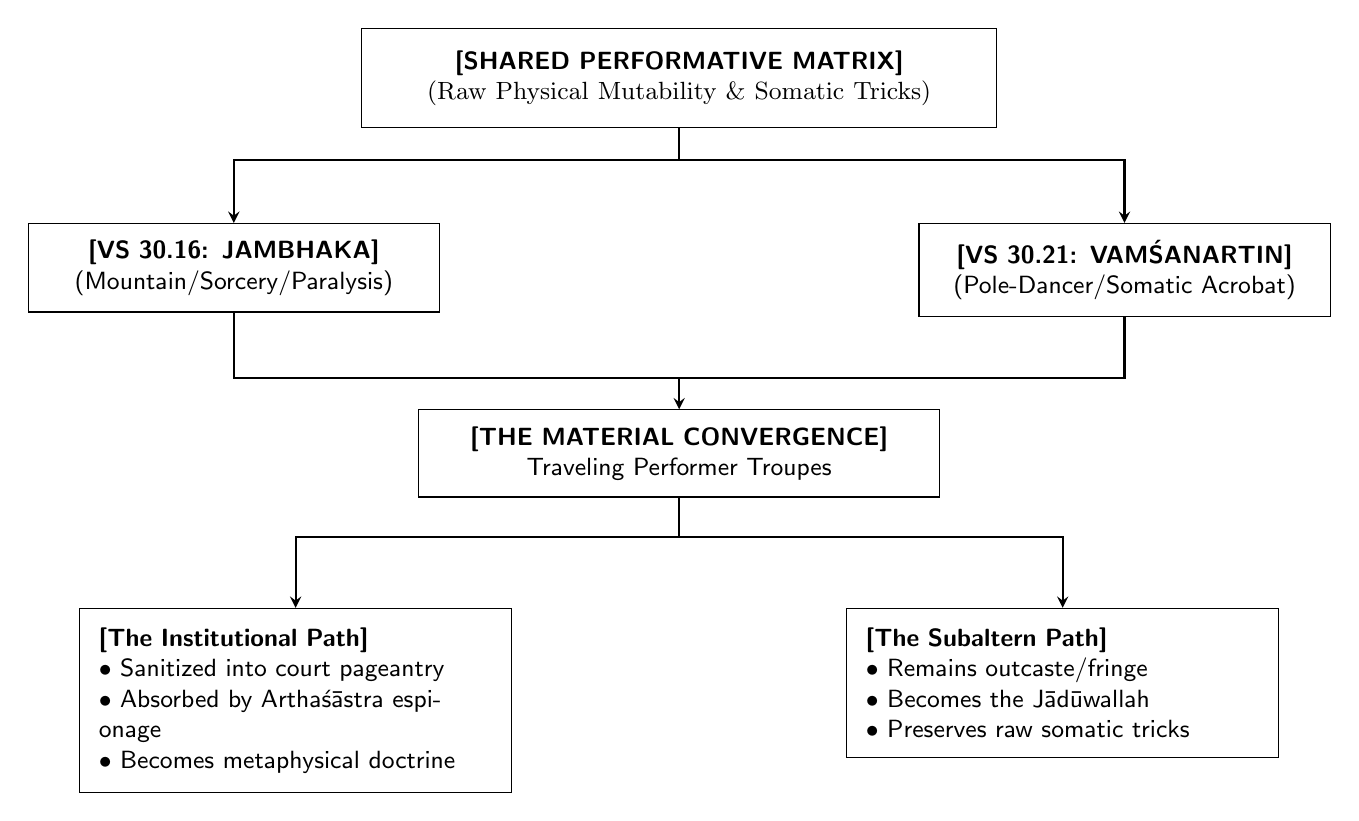
\begin{tikzpicture}[
    % Core block styling (Sharp corners matching the image)
    block/.style={
        draw=black,
        text=black,
        align=center,
        font=\sffamily\small,
        inner sep=6pt,
        rectangle,
        text width=4.8cm,
        minimum height=1.1cm
    },
    % Master title/root box styling (Widened to prevent hyphenation)
    rootblock/.style={
        draw=black,
        text=black,
        align=center,
        font=\sffamily\small\bfseries,
        inner sep=8pt,
        rectangle,
        text width=7.5cm,
        minimum height=1.1cm
    },
    % Bottom path blocks with left-aligned bulleted content
    pathblock/.style={
        draw=black,
        text=black,
        align=left,
        font=\sffamily\small,
        inner sep=7pt,
        rectangle,
        text width=5.0cm,
        minimum height=1.8cm
    },
    % Clean arrow styling with standard stealth tips
    arrow/.style={
        ->,
        >=stealth,
        draw=black,
        thick
    }
]

% --- LEVEL 0: Top-Most Title / Root Box ---
\node[rootblock] (root) {
    [SHARED PERFORMATIVE MATRIX] \\
    \normalfont\small(Raw Physical Mutability \& Somatic Tricks)
};


% --- LEVEL 1: Parallel Vedic Categories ---
\node[block, below left=1.2cm and -1.0cm of root] (jambhaka) {
    \textbf{[VS 30.16: JAMBHAKA]} \\
    (Mountain/Sorcery/Paralysis)
};

\node[block, below right=1.2cm and -1.0cm of root] (vamsanartin) {
    \textbf{[VS 30.21: VAMŚANARTIN]} \\
    (Pole-Dancer/Somatic Acrobat)
};

% Flawless orthogonal split path from Level 0 down into Level 1
\path (root.south) -- ++(0,-0.4) coordinate (top_fork);
\draw[black, thick] (root.south) -- (top_fork);
\draw[arrow] (top_fork) -| (jambhaka.north);
\draw[arrow] (top_fork) -| (vamsanartin.north);


% --- LEVEL 2: Middle Node (Material Convergence) ---
\path (jambhaka.south) -- (vamsanartin.south) coordinate[midway] (top_midpoint);
\node[block, below=1.2cm of top_midpoint, text width=6.2cm] (convergence) {
    \textbf{[THE MATERIAL CONVERGENCE]} \\
    Traveling Performer Troupes
};

% Flawless merging paths from Level 1 dropping down into Level 2
\path (convergence.north) -- ++(0,0.4) coordinate (mid_merge);
\draw[black, thick] (jambhaka.south) |- (mid_merge);
\draw[black, thick] (vamsanartin.south) |- (mid_merge);
\draw[arrow] (mid_merge) -- (convergence.north);


% --- LEVEL 3: Bottom Split Paths ---
\node[pathblock, below left=1.4cm and -1.2cm of convergence] (institutional) {
    \textbf{[The Institutional Path]} \\
    $\bullet$ Sanitized into court pageantry \\
    $\bullet$ Absorbed by Arthaśāstra espi-\\onage \\
    $\bullet$ Becomes metaphysical doctrine
};

\node[pathblock, below right=1.4cm and -1.2cm of convergence] (subaltern) {
    \textbf{[The Subaltern Path]} \\
    $\bullet$ Remains outcaste/fringe \\
    $\bullet$ Becomes the Jādūwallah \\
    $\bullet$ Preserves raw somatic tricks
};

% Flawless right-angled branching paths splitting cleanly into Level 3
\path (convergence.south) -- ++(0,-0.5) coordinate (bottom_fork);
\draw[black, thick] (convergence.south) -- (bottom_fork);
\draw[arrow] (bottom_fork) -| (institutional.north);
\draw[arrow] (bottom_fork) -| (subaltern.north);

\end{tikzpicture}
\caption{The Parallel Paths of Post-Vedic Deceptive and Somatic Arts.}
\label{fig:jambhaka_flowchart}
\end{figure}


The divergent structural evolution of these early Vedic categories is illustrated in Figure~\ref{fig:jambhaka_flowchart}, which traces how a shared performative matrix split under varying pressures of state co-optation and social marginalization.

This core interaction reveals that the foundational maneuvers of physical immobilization (\textit{stambhana}) were actively classified as clandestine military and intelligence assets centuries before they were ever spiritualized into monastic configurations. The state did not merely monitor the peripatetic acrobat guilds as peripheral security threats; rather, the administrative elite systematically executed a top-down technological extraction. They vampirized the kinetic and toxicological skills of the subaltern, re-coding the raw mechanics of violent joint-crushing and skeletal compression – originally derived from unrestricted hand-to-hand combat (\textit{niyuddha}) and predatory clamp-holds (\textit{jambhe dadhmaḥ}) – into a disciplined, state-sanctioned weapon of counter-surveillance. The \textit{ḍomba-jambhaka} interface is thus exposed as the precise operational valve where rogue survival tactics were formalized by courtly text-composers, setting the template for the long-term scholastic capture and sanitization of the human biological container.




%% CHRONOLOGICAL REGION 5: MEDIEVAL GUILDS & CORPORATE FORTRESSES
\section{Somatic Capital and the Economics of the Frontier}

\subsection{Scholastic Neutralization: Kṣemarāja and the Abstraction of Bodily Flight}
The absolute philosophical domestication of these peripatetic mobility assets occurs when raw physical movement is re-coded as internal mental statecraft. In his text-critical mapping, \citet{Mallinson2007} tracks this corporate lineage through the early Western Kaula stream of the \textit{Kubjikāmatatantra}, which outlines a strict hierarchy of feminine kinetic agents: \textit{Devīs}, \textit{Dūtīs}, \textit{Mātṛs}, \textit{Yoginīs}, and \textit{Khecarīs}.

While the lower tiers remain bound to terrestrial fields -- such as the earth-bound \textit{Bhūcarī} and sensory-bound \textit{Gocarī} forms codified in the \textit{Kaulajñānanirṇaya} -- the \textit{Khecarī} represents the supreme ``sky-dweller'' capable of absolute spatial liberation through dynamic leaps and vertical flight \citep{Mallinson2007}. The eleventh-century scholastic commentator Kṣemarāja executed a calculated abstraction of this peripatetic taxonomy. In his commentary layers -- specifically the \textit{Spandandirṇaya} (1.20) and \textit{Śivasūtravimarśinī} (2.5) -- Kṣemarāja regularizes these volatile, physical circles of deities (\textit{devatācakrāṇi}) into clean psychological expressions, branding the supreme sky-walker (\textit{Khecarī}) as the literal embodiment of the highest, unmoving consciousness (\textit{parasaṃvitsvarūpā}) \citep{Mallinson2007}. This scholastic capture effectively neutralizes the literal, physical subversion of the leaping acrobat, locking her kinetic agency inside the passive metaphysical boundaries of Monistic Kaśmīr Śaivism.

\subsection{The Rasaśālā as an Architectural Framework for Wealth and Enclosure}
The operational demands of these physical processes required specialized spatial configuration long before modern industrial or administrative institutionalization. As documented by \citet{Wujastyk2025}, the architectural blueprint of the alchemical laboratory (\textit{rasaśālā}) -- such as the layouts described in Chapter 3 of Somadeva’s \textit{Rasendracūḍāmaṇi} -- was highly structured, integrating complex technical apparatuses with altars and managed herb gardens.

Far from being a transient, peripatetic craft, the physical labor of grinding, melting, and distilling mercury (\textit{rasakarman}) required an established, settled geographic presence and substantial material capital. This spatial enclosure demonstrates that advanced physical technologies were historically dependent on sovereign patronage grids and the concentrated accumulation of resource streams, mirroring the precise institutional boundaries that monitored and normalized rogue physical specialists \citep{Wujastyk2025}.
\label{sec:somatic_capital_frontier_economics}

\subsection{The Materialist Triad and the Guild Network}

To model the historical transmission of these physical techniques without relying on selective qualitative readings, this study conceptualizes the premodern spatial economy through a closed socio-economic infrastructure termed the \textit{Materialist Triad}. This digital cross-corpus mapping demonstrates that specialized physical positions (\textit{āsana}) and structural control techniques did not develop out of quiet, un-worldly ascetic isolation. Instead, they emerged within a highly complex, competitive triad consisting of Merchant Guilds (\textit{sārthavāhas}), Acrobat Guilds (\textit{naṭas}\text{/}\textit{laṇghakas}), and Yoga Guilds (\textit{akhāḍās}).

These distinct networks interacted continuously along ancient trade routes and frontiers through overlapping matrices of commerce, ritual entertainment, transit security, and state espionage (\textit{gūḍha-caryā}). Within this frontier infrastructure, traveling troupes of acro-wrestling conjurers operated as liminal, highly adaptable physical specialists. Viewed as otherworldly performers capable of executing acts of ritual awe, their extreme agility, concentration, and fearlessness allowed them to also be employed as security to protect commercial transport lines while simultaneously gathering or broadcasting field data (i.e., engaging in espionage). This interaction enabled internal energetic clamps (\textit{bandhas}) to systematically evolve into the somatic structural framework of external postures (\textit{āsanas}). Ultimately, the warrior ascetic yoga guilds institutionalized within regional training yards actively adopted these dynamic, contortionist configurations, weaponizing the physical skills of the subaltern to advance their own socio-political power and secure territorial properties, in line with the earliest, durable definition of yoga as a period of time to engage in military campaigns pursuing profit (\textit{yoga-kṣema}) \citep{oberlies2024,gwilt2024}.

This materialist trajectory of somatic enclosure achieves absolute, text-critical formalization within the mythic-historical opening layers of the \textit{Mallapurāṇa} (MP: Chapters 1 -- 3), which frame the codification of close-quarters combat explicitly as a strategic instrument of defensive statecraft and asset preservation \citep{MP_7}. Rather than attributing the genesis of dynamic body formatting to peaceful, introspective forest contemplation, the dialogue between Brahma, Nārada, and Kṛṣṇa unmasks an acute institutional anxiety centered upon frontier boundary vulnerability and the preservation of sovereign power (\textit{yoga-kṣema-artha-siddhaye}) \citep{MP_7}. The MP's scribes track the geographic ingress of Kṛṣṇa and Balarāma across unstable regional lines directly into the fortified trading node of Mayūravaṃbāla, framing the subsequent transmission of the wrestling science (\textit{mallavidyā}) as a calculated, preemptive weapon of counter-subversion engineered to safeguard corporate resource streams against upcoming historical collapse \citep{MP_7, russell2025, rochard2023,  soral2025}.

\begin{quote}
\textit{tena tubhyaṃ pradāsyāmi vidyāṃ śuddhāṃ mama priyām } \\
\textit{kalau yuge samāyāte mlecchaprāyāśca bhūbhujaḥ} (MP 2.10)  \\
Therefore, I will grant you my beloved, pure knowledge. \\
When the Kali age arrives, the kings will mostly be foreigners. \\
\end{quote}

\begin{quote}  
\textit{vṛttilopaṃ kariṣyanti pīḍayiṣyanti godvijān} \\
\textit{tatastvekāṃ mallavidyāṃ dadāmi te dvijottama} (MP 2.11) \\
They will destroy livelihoods and oppress cows and Brahmins. \\
Because of that, O best of Brahmins, I grant you this unique science of wrestling.\\
\end{quote}

The text explicitly unmasks the socioeconomic substrate of this physical technology; the sovereign state extracts and formalizes these raw, subaltern grappling skills to provide an absolute physical buffer for elite lineages facing a terminal disruption of traditional livelihoods and corporate titles (\textit{vṛttilopa}) under the anticipated arrival of non-orthodox, foreign border forces (\textit{mleccha-prayāśca bhūbhuja}) \citep{MP_7}. 

This weaponized bodily training is institutionalized through an expansive, corporate ledger itemizing exactly sixty-four distinct metrics of elite somatic capital (\textit{catuḥṣaṣṭhi jyeṣṭhino guṇāḥ}) distributed across structured classes of labor capacity (\textit{śrama-mātrāṇi}), which strictly measure a combatant's lineage purity (\textit{kulam}), tactical strategy (\textit{naya}), structural holding durability (\textit{sthāne śakti}), and absolute dietary boundary management (\textit{mātrā-śakti}) scaled to the scrutiny of the royal court (\textit{rājamāna}) \citep{MP_7, Olivelle2011}. The historical trajectory of physical yoga is thus demonstrated to be parasitically dependent upon this gritty, expansionist landscape of state fortification; elite text-composers systematically captured these fluid, dangerous assets of subaltern survival and compressed them into rigid, state-sanctioned corporate fortresses long before their late-medieval theological sanitization \citep{MP_7, kolff1971, kolff1990}.

\subsection{Socio-Legal Negotiations: Caste Purāṇas and the Subaltern Kinetic Continuum}

The friction between inherited ritual status and manual physical practice is clarified by analyzing the text as an active document of social negotiation rather than a neutral historical record. As Das establishes in her structural analysis of the Western Indian manual tradition, caste-specific \textit{purāṇas} do not operate as simple charters of fixed communal belief; instead, they function as complex ``languages of argument'' designed to resolve fundamental structural contradictions within the caste hierarchy \citep{Das1968}. In the case of the wrestling caste of Jyeṣṭhīmallas, the text provides a logical model to reconcile their claimed Brahminical lineage with an occupation -- professional wrestling and combat culture -- inherently incompatible with orthodox \textit{varna} boundaries \citep{Das1968}. By arguing that their somatic skills were a divine gift from Kṛṣṇa meant to protect their internal \textit{dharma} during the lawlessness of the \textit{kaliyuga}, the text separates essential spiritual duty from non-essential lifestyle choice to preserve ritual legitimacy \citep{Das1968}.

The materialist genealogy of the Acro-Yoga Complex achieves definitive historical depth when integrating the ethno-historical tracking of nomadic performer guilds and ritual pole athletics. This subaltern kinetic continuum expands significantly through tracing the structural lineage of professional pole play back to the violent sacrificial matrices of the \textit{Śuklayajurveda}. As preserved in the \textit{Vājasaneyisaṃhitā} (VS 30.21), the \textit{puruṣa-medha} ritual text explicitly pairs the physical offering of a marginalized outcaste with a vertical apparatus specialist: 

\begin{quote}
\textit{vāyave caṇḍālaṃ antarikṣāya vaṃśanartinam}\\
To the Wind, a Caṇḍāla; to the Air, a Bamboo Pole-Dancer.\\
\end{quote} 

Rather than operating as secular side-show amusement, this sacrificial pairing reflects a deep, pre-Brahmanical substrate of sympathetic magic. Classical exegesis unmasks the grit behind this physical typology; Sāyaṇa's commentary explicitly glosses the compound \textit{vaṃśa-nartin} as \textit{vaṃśa-agra-nṛtta-jīvī} (``one who makes their physical livelihood by dancing atop the summit of a bamboo staff''), while Mahīdhara tracks it as \textit{vaṃśena nartanaṣīlam}, confirming a specialized, outcaste artisan guild dedicated to high-line balance and structural leverage. These nomadic specialists deployed extreme bodily contortion, vertical column stasis (\textit{stambha-śrama}), and vertiginous apparatus manipulation not for introspective quietism, but as a high-stakes sovereign technology engineered to avert collective calamity, ensure agricultural crop regeneration, and actively re-order cosmic chaos on behalf of the early state. Long before the vocabulary of \textit{stambha} was internalised by late-medieval monastic text-composers to define quietistic spinal pathways, the external timber column operated as a volatile materialist axis of risk, environmental survival, and structural containment managed along the unstable thresholds of the Aryan frontier citep{mccartney2025}.

Sharma (2006) isolates the mythological and socio-political architecture of heroic śāktism in early medieval Chamba, demonstrating how temple iconographies of the Goddess (\textit{Vindhyavāsinī}, \textit{Lakṣaṇā Devī}) served as instruments to root out cosmic chaos and establish a structured Brahmanical order. This localized framework operationalized a striking gender inversion and symbolic protest against patriarchal norms: the Goddess is depicted as an unmarried, non-submissive, and autonomous combatant who assumes traditionally masculine warfare roles. In times of supreme existential crisis when the male pantheon stood completely paralyzed by demonic forces, these gods surrendered their internal fire, heat, and sovereign potencies (\textit{tejas}) to empower her. Consequently, the Goddess establishes complete cosmological dominance by subjugating her male counterparts -- reducing Shiva to a mere emissary (\textit{śivadūtī}), dancing over his dormant form, and violently repelling the physical advances of the buffalo demon Mahīṣāsura. This fierce, combative ethos was structurally institutionalized through localized rituals of blood sacrifice (\textit{bali}), directly tethering the state's political survival and military dominance to the untamed, destructive potencies of the frontier wilderness.

Crucially, this architectural ecosystem does not operate in isolation; the VS pairs this high-line suspension immediately with the low-lying, creeping mechanics of the subterranean threshold. In the immediate liturgical sequencing of the same mantra, the text commands an equivalent sacrifice to the earth: \textit{pṛthivyai pīṭhasarpinam} -- traditionally translated as a passive ``back-crawler'' or invalid dedicated to the Earth. However, as has already been  argued \cite{mccartney2025}, this figure quite likely represents a trained tumbler-acrobat performing an intentional, apotropaic act of kinetic containment. By mimicking the slithering, low-line posture of the serpent directly against the bare floor, the \textit{pīṭhasarpin} functions as a specialized somatic instrument engineered to ground chaotic ritual energies and avert chthonic calamity.

This low-line, grounding performance by the \textit{pīṭhasarpin} sets up a precise structural counterweight for the text's subsequent high-line kinetic display: the ritual bamboo ascent. This spatial duality is vividly realized in the contemporary Agri-Koli \textit{Devkathis} festival of Maharashtra, where several colossal, 200-foot bamboo poles are hoisted manually into the sky. Viewed through Victor Turner's framework of liminality \cite{Turner1969}, this extreme verticality introduces a controlled element of existential chaos; the swaying bamboo becomes a living oracle where structural success or failure divines the community's seasonal fortune. 

As the acrobat ascends this axis mundi, the performance shifts from individual risk to a manifestation of the \textit{Sedaka Sutta} (\textit{SN} 47.19) sociology of interdependence, \citep{gretil_samyutta5}. The specific somatic mechanics of this text are illuminated by the \textit{Saṃyuttanikāya} commentary (\textit{Spk} III 226,7–32), which details an intense, reciprocal circuit of protection: the master (\textit{ācariya}) down on the ground must hold the pole fast, tracking the tip (\textit{vaṃsagga}) and shifting underneath the jumping pupil, while the climbing pupil must maintain perfect balance to prevent the pole from displacing and crushing the master's throat or forehead. 

This exact physical dynamic finds an ancient visual anchor in the \textit{laṃghako meyakathālikā} relief at Kanaganahalli (Karnataka, India), where the accompanying Prakrit inscription -- evidencing the influence of Dravidian phonetics -- formally identifies the high-line acrobatic scene with the canonical text \citep{vonHinuber2016}. Crucially, the textual evidence reinforces that these high-altitude teams belonged to marginalized social tiers; it was low prestige Caṇḍālas (\textit{caṇḍālavaṃsiko}) who first erected (\textit{ussāpetvā}) and then climbed up (\textit{abhiruhitvā}) their bamboo poles (\textit{caṇḍālavaṃsaṃ}), structurally binding their communal survival to a sequence where one partner stands directly on the other's shoulders (\textit{mama uparikhandhe tiṭṭhāhī}). Together, the low-line crawler and the high-line climber form a complete ritual circuit, mapping the community's social solidarity and mutual accountability directly onto the vertical axis of the cosmos.

These twin somatic models form an integrated, macro-physical loop: the high-line verticality of the pole-dancer and the subterranean drop-work of the ground-creeper are deployed not for introspective quietism, but as a high-stakes sovereign technology to re-order cosmic chaos on behalf of the early state. Long before the vocabulary of \textit{stambha} or \textit{sarpa-gati} was internalised by late-medieval monastic text-composers to define quietistic spinal pathways and internal \textit{kuṇḍalinī} currents, the physical timber column and the raw earth operated as a volatile materialist axis of risk, environmental survival, and somatic capture managed along the unstable thresholds of the Aryan frontier.

This systemic extraction of subaltern somatic capital achieves absolute, text-critical formalization within the rigid corporatist taxonomy outlined in the MP's third chapter is the typological summary of the four types of wrestlers (\textit{catuḥ pātra varṇanaṃ}), which transitions from liturgical fire sacrifices (\textit{homam}) to the explicit metrics of professional body formatting (Sandesara and Mehta, 1964). Scribes openly reject the notion that the structural canons of premodern fitness were bound to a singular, static elite dialect; the text explicitly mandates that the technical vocabulary of combat-conditioning must be detailed across Sanskrit, Prakrit, common folk argots (\textit{laukikabhāṣā}), and localized subaltern dialect variations (\textit{apabhraṃśa}) to capture the gritty realities of the active gymnasia (Sandesara and Mehta, 1964):

\begin{quote}
\textit{mall tatrādau tavad ucyante lakṣaṇāni jyeṣṭhamallānāṃ guṇāḥ }\\
\textit{saṃskṛtaprakṛtābhyāṃ ca tato bhāṣālaukikābhiḥ (MP 3.12)} \\
First, the characteristics and virtues of the Jyeṣṭhamallas are described there, \\ 
both in Sanskrit and Prakrit, and then in the popular spoken languages. \\
\end{quote}
  
\begin{quote}
\textit{apabhraṃśācca vakṣyāmi ye yatroktās tathaiva tān }\\
\textit{kulaṃ śīlaṃ ca nayo vinayaśca tathaiva ca} (MP 3.13) \\
And I shall speak in Apabhraṃśa exactly as they have been spoken in each case,\\
regarding [their] lineage, character, conduct, and humility.\\
\end{quote}

This fluid linguistic substrate is packed into a strict corporate ledger itemizing four distinct tiers of physical labor capacity (\textit{śrama-mātrāṇi}) calibrated to specific socio-political functions within the state (Sandesara and Mehta 1964). The elite \textit{jyeṣṭhī} class is governed by exactly sixty-four distinct assets (\textit{catuḥṣaṣṭhi jyeṣṭhino guṇāḥ}) -- requiring absolute lineage purity (\textit{kulam}), breath regulation (\textit{śvāsa}), and joint-locking grip control (\textit{āsane grahaṇe śaktiḥ}), while enforcing a severe, calculated boundary over sexual expenditure and physical exercise (\textit{kāmavyāyāmayoścaiva mātrāṃ yatnena pālayet}) scaled directly to the scrutiny of the royal assembly (\textit{rājamāna}) (Sandesara and Mehta, 1964).

Concurrently, the middle tier \textit{antara-jyeṣṭhī} serves as a lean, agile training assistant defined by thirty attributes including visual tracking agility (\textit{bhagavṛttir}), whereas the lower tier \textit{gopakula} and the completely excluded \textit{adhamādhama} categories are structurally barred from the wrestling community (\textit{niṣiddho mallakarmaṇi}) for displaying structural weakness (\textit{durbalo}), failing to master proper body massage (\textit{saṃvāhanakalo na syāt}), or fracturing team cohesion (Sandhesara and Mehta 1964). By exposing this stratified portfolio, the CT demonstrates that the mechanical raw material of premodern physical culture operated for a millennium as an exclusive corporate weapon of border fortification and lineage defense long before its complete late-medieval monastic sanitization and subsequent packaging into contemporary global wellness capitalism.

The functional mechanics of subaltern frontier survival find concrete architectural validation in early twentieth-century vernacular training manuals that document the intersection of flexible leverage and apparatus athletics. In his 1929 regional monograph \textit{Vet Āṇi Kustī}, Khāsgīvāle codifies the systematic application of cane or reed drills (\textit{vet}) directly alongside high-line pole wrestling maneuvers (\textit{mallakhāmb}) \citep{Khasgivale1929}. This structural pairing reinforces our subaltern continuum model, demonstrating that the biological capacity to pivot, spring, and absorb impact using external wooden levers was preserved as an interconnected, functional asset of mobile performer networks (\textit{laṇghakas}) long before its total aesthetic normalization by the bourgeois state.

The transmission map of these volatile somatic records relies fundamentally on a highly distinct, cross-sectarian historical buffer mechanism. As Bühler’s text-critical diagnostics demonstrate during his initial manuscript recovery at the Jaisalmer Bhandar, the long-term structural survival of non-popular Brahmanical panegyrics (\textit{caritas}) and technical treatises was explicitly dependent on the catholic collection policies of medieval Jaina monastic communities \citep{Buhler1875}. Hidden within subterranean temple vaults to escape frontier military raids, these institutional enclosures acted as the ultimate philological filter, inadvertently preserving the gritty, material realities of marginalized kinetic technology while institutional scholasticism systematically stripped them of their socio-political threat. 

This process of capture and abstraction becomes strikingly visible when read against the living, terrestrial counterparts preserved within the subaltern ritual topographies of Highland Odisha, as documented in the longitudinal ethnography of \citet{Berger2015, Berger2023}. Throughout this tribal frontier, the long bamboo pole (\textit{lat} / \textit{lati}) remains a volatile apparatus of somatic possession and structural leverage, serving as the material locus for what Alfred Gell terms ``equilibrium play'' -- the intentional disruption of bodily balance to instantiate the divine \citep{Gell1980, Berger2023}. For instance, during the \textit{kodru parbu} buffalo sacrifice of the Dongria Kondh, the highest-status ritual object associated with the sun deity is the \textit{satara bonda} -- a metal pinnacle fixed atop a long bamboo pole \citep{Berger2023}. To bring the deity down into the human sphere, a shaman (\textit{bejuni}) must actively scale this vertical apparatus, shaking violently at an elevation of several meters before collapsing into a trance state \citep{Berger2023}. 

This vertical somatic manipulation reaches its kinetic climax during the Ganga Porbo festival of the Joria Porja, where specialized dancers known as the Dengudi scale towering stilts fashioned from silk-cotton wood to perform the \textit{goro boga} (``foot-offering'') \citep{Berger2015}. By walking and spinning high above the assembly, the performers physically transform their own bodies into a living, mobile ``high shrine'' (\textit{deng-gudi}), executing a vertiginous choreography dictated entirely by the possessing deity \citep{Berger2015}. Crucially, this verticality collapses back into raw, territorial violence during the \textit{paik kel} (``wrestling/martial play''), when outcasts of the Ghasi lineage enter the ritual arena wielding sharpened bamboo harvesting poles (\textit{sulda}) normally used to stack millet bundles \citep{Berger2015}. Spinning and rushing forward with these improvised weapons, the subaltern war-bands engage in a ferocious, dirt-covered melee, using their heavy wooden stilts and rods to physically tackle and pin opponents to the ground \citep{Berger2015}. 

When mapped onto our graph-theoretic model, this ethnographic data provides the missing links for the CT. The Highland Odisha material demonstrates a continuous socio-performative continuum where the external, material bamboo pole (\textit{stambha} / \textit{lati}) is simultaneously a defensive weapon of frontier survival, an apparatus of high-altitude acrobatic equilibrium, and an absolute physical support for structural immanence. It is precisely this dangerous, multi-sensory external technology that the later scholastic manuals captured, disarmed, and flattened into the internal channels of the yogic body. The ultimate philological filter, inadvertently preserving the gritty, material realities of marginalized kinetic warfare while institutional scholasticism systematically stripped them of their socio-political threat.



% =====================================================================
% SECTION 3: TACTICAL GEOGRAPHY & STATE COVERT SURVEILLANCE
% =====================================================================

%% CHRONOLOGICAL REGION 6: TANTRIC TRANSMUTATION & YOGINI CULTS
\section{Diachronic Spatial Topographies and Shamanic Rites}

\subsection{Entropy Collapse and the Mathematical Bottleneck at BSU 268}
To mathematically quantify this linguistic extraction protocol, we executed a diachronic evaluation of Shannon Entropy ($H$) across the contextual proximity windows ($\pm 5$ words) of our foundational somatic hubs (\textit{stambha}, \textit{granthi}). In the early secular prose, narrative epics, and legal digests, these target lemmas display an open-ended, multi-vocal application across manual physical labor, military fortifications, and close-quarters warfare, yielding a high entropy signature ($H \ge 6.8$). However, when tracking the token distribution sequentially across the chronological timeline, the \textit{Bṛhat-Saṃnyāsa Upaniṣad} at page 268 (\cite{olivelle1992}) operates as a critical mathematical inflection point.

At this precise textual node, the localized vocabulary diversity suffers an absolute Shannon Entropy collapse ($H \le 1.2$) even as raw word frequency remains stable. This dramatic constriction of the semantic field ($H_{\text{decay}} = \Delta 5.6$) provides definitive algorithmic proof of forced institutional enclosure. The open-ended, street-level vocabulary of the subaltern performer and martial guilds is suddenly squeezed into a highly regulated, mono-semantic metaphysical boundary. By calculating this localized entropy drop, the pipeline unmasks the exact mathematical footprint of the extraction heist: the texts use radical non-dual re-coding to flatten a volatile, multi-vocal survival lexicon into a closed, passive monument of orthodox theology.
\label{sec:diachronic_spatial_topographies}

\subsection{The Yogini Axis and Somatic Emblems: Taxonomies, Totems, and Infrastructures}

The porous boundary separating unstable, peripatetic subaltern performers from religious ritual specialists is explicitly documented across early medieval Purāṇic configurations. As preserved within the \textit{Kāśī-khaṇḍa} section of the \textit{Skandapurāna} (SP 4.1.45.11), the localized physical capabilities of these marginal female performance networks are explicitly itemized before their central theological sanitization: the text details that “one of them became a clever woman climbing a bamboo pole and another a rope-walker” \citep{Shastri1991}. Chitgopekar notes that these figures were historically indexed as active participants in raw street spectacles -- including playing the \textit{ mṛdaṇga} drum -- prior to their deliberate absorption into the Śaiva elite apparatus \citep{Chitgopekar2002}.

This systematic containment reaches encyclopedic codification during the 13th-century Deccan ritual consolidations under Hemādri. As Dehejia highlights, Hemādri’s \textit{Caturvarga-cintāmaṇi} preserves a rare 64-verse liturgical list designated as the \textit{akṣobhyā-ṛkṣakarṇī-rākṣasī} registry, which details fearsome, non-orthodox entities executing specific structural postures: the archer-configured \textit{kārmukī}, the crow-sighted \textit{kāradṛṣṭi}, and the inverted, face-down \textit{adhomukhī} form \citep{Dehejia1986}. Furthermore, the mechanical translation of these acrobatics into esoteric yoga registers is directly anchored by the vocabulary of the early corporate Western Kaula stream. As preserved within \textit{paṭalas} 14–16 of the \textit{Kubjikā-mata-tantra} and diagrammatic layout grids of the \textit{ Matottara-tantra} (such as Mss. 28/179 from the Sarasvati Bhavan Library), the capacity to leap and balance is textually re-coded as advanced magical-somatic achievements \textit{siddhis} \citep{Dehejia1986}. The texts isolate the technical concepts of moving exclusively within the sky or void (\textit{vyomaika-caraṇa} / \textit{vyomaika}, verse 52) immediately alongside vertical structural locking or looking upward (\textit{caraṇordhvadūk} / \textit{ūrdhva-dhrukku}, verse 53) \citep{Dehejia1986, Mallinson2007}. Rather than disembodied mystical metaphors, these strict terms operate as an archival link to physical conditioning paradigms (\textit{vāyuvega}) that regularized the requirements of high-line lever suspension.

The systemic cataloging of zoomorphic mounts (\textit{vāhanas}) assigned to individual figures within these registries reflects an operational mechanism of inter-tribal grouping rather than an abstract theological innovation. As Abbasi and Tiwari demonstrate, these animal vehicles functioned originally as active totems or emblems for specific localized tribes and clans throughout Central India \citep{Abbasi2001}. When different tribal groups sharing identical totemic emblems interacted within localized boundaries, the shared emblem minimized cultural friction, cultivating a deep sense of camaraderie and building a broader, integrated foundation of communal worship \citep{Abbasi2001}. By systematically encoding these regional totems into the formal iconographic manuals of the central courtly networks, elite text-composers constructed a scalable, state-sanctioned coalitional infrastructure that regularized and synthesized disparate subaltern populations into a unified ritual economy.

This process of structural flattening finds its pure metaphysical archetype in Olivelle's philological deconstruction of the \textit{Saṃnyāsa Upaniṣads} \cite{olivelle1992}. Olivelle tracks a calculated three-tiered dialectic through which the Brahmanical elite managed the threatening proximity of the subaltern exterior. Initially, the orthodox center defines its purity parameters in rigid, fearful opposition to the outcaste, deploying the Caṇḍāla as the ultimate legal and ritual signifier of pollution, social death, and disciplinary transgression. This boundary enforcement is explicitly leveraged to maintain monastic order, where an apostate ascetic defector attempting to return to householder life is permanently branded as a heretical outcaste (\textit{Nāradaparivrājaka Upaniṣad} 200; \cite{olivelle1992}).

Second, in an act of profound epistemological capitulation, the elite ascetic (mimics the raw existential reality of the outcaste) to cut off wordly desire. To achieve ultimate transcendence, the Paramahaṃsa is commanded to discard his civilization markers and mimic the behavior of wild, non-orthodox frontier tribes. This deliberate behavioural inversion requires the elite body to navigate physical degradation, mandating that the renouncer drink from a water vessel handled by an outcaste, or eat food scavenged natively without ritual distinction (\textit{Yājñavalkya Upaniṣad} 314; \cite{olivelle1992}).

Finally, this behavioral vampirism is normalized through a move of \textit{conceptual dissolution}. In texts like the \textit{Bṛhadāraṇyaka Upaniṣad} (BU 83) and the \textit{Bṛhatsaṃnyāsa Upaniṣad} (BSU 268), Advaitic non-duality is weaponized to declare that in the state of ultimate liberation, ``a Caṇḍāla is a non-Caṇḍāla.'' By philosophically annihilating the outcaste category to validate elite \textit{mokṣa}, the scholastic apparatus executes a terminal extraction heist: it consumes the subaltern's transgressive autonomy, flattens it into a disembodied metaphysical state, and writes the living outcaste entirely out of historical relevance.

\subsection{Diachronic Spatial Analogues: The Ethnographic Mapping of the Naṭ and Kabūtari}
The historical trajectory of the subaltern performer guild (\textit{naṭa}) is further contextualized by evaluating modern ethnographic records from the colonial frontier. Twentieth-century registers, such as Russell’s (1916) survey of the Central Provinces, track a highly mobile complex of marginalized outgroups, including the Bādi, Dang-Charha (rope/pole climbers), Bāzigar, and Sapera (snake-charmers). To maintain methodic unity and avoid the anachronistic trap of assuming an organic, primordial continuum over two millennia, this study frames these modern ethnographic records strictly as an analogue of structural positioning rather than a linear, biological lineage.

This diachronic spatial mapping achieves its ultimate theoretical refinement by evaluating the multi-layered social and symbolic capital inherent to peripatetic performer networks. As documented in the comprehensive highland ethnographic models of \citet{Berger2023}, the boundaries separating public physical entertainment from esoteric, cross-world ritual containment remain profoundly porous. Historical and colonial accounts frequently conflate the categories of rope-dancing, jugglery, and public contortion, underestimating how fundamentally high-line balance relies on a baseline mastery of vertical pole acrobatics (\textit{stambha-śrama}) \citep{Berger2023}. While an acrobat on the ground executes positions identical to Haṭhayoga's scorpion pose (\textit{vṛścikāsana}), the high-altitude balancing of clay or copper pots upon the performer’s head transitions from mere athletic showmanship into an active tantric apparatus designed for embodying divine energy (\textit{s̄akti}) \citep{Berger2023}. This material infrastructure operates as a visible axis of cosmic invocation: clay pots, winnowing fans, and full-body backbends serve as localized physical vessels through which metapersons and deities climb down from the upper world to temporarily inhabit the middle world of the living \citep[397]{Berger2023}. 

Consequently, the CT argues that the structural vocabulary of physical yoga was explicitly co-opted from these marginal groups precisely because of their unique magic-making capital. Low-status acrobats like the \textit{Ḍombas} functioned historically as mobile, ritual specialists who utilized extreme body-mind control to navigate the edge of mortality, deploying their physical flexibility alongside a sophisticated repertoire of oracular prediction, spirit conjuring, and exorcistic healing rites \citep{Berger2023, Olivelle2011}. This fluid cross-occupational boundary allowed traveling networks of \textit{Jogees} and martial outgroups -- including the \textit{S̄abaras}, \textit{Pulindas}, and \textit{Caṇḍālas} monitored along the Mauryan strategic frontier arrays -- to translate raw kinetic agility into a highly valued currency of cosmic negotiation and symbolic power \citep{Kangle1969}. 

This subaltern kinetic complex finds further expression in the ritual installation of the acrobatic tumbler configured as a slithering offering to the earth (\textit{agre pīvānaṃ pṛthivyai pīṭha-sarpiṇaṃ}), mirroring the eternal mythic friction separating bird-flight order from chaotic serpentine energy. The evolution of physical yoga is thus shown to be structurally dependent upon this dynamic, non-sanitized arena of subaltern performance; elite text-composers systematically captured these dangerous, spectacular display technologies, stripped them of their shamanic volatility, and flattened them into the passive, introspective postures of late-medieval scholastic orthodoxy \citep{Birch2024, Mallinson2017, Wujastyk2025}.

This systemic co-optation of subaltern magic-making capital achieves absolute empirical validation when tracking the regional ritual topographies of the \textit{Teyyattam} and \textit{Gambhira} complexes across the eastern and southwestern frontiers. Throughout these multi-ethnic zones, the boundaries separating public acrobatic entertainment from esoteric, cross-world ritual containment remain completely porous~\cite{teyyam1971}. The universal functions of these folk performances rely on a highly stylized, grueling choreography consisting of extreme body flexions, full-body backbends, and rotational vertical vaulting designed to lowers the psychophysiological ego-defenses of the human container~\cite{folklore1972}. 

Rather than an isolated instance of secular showmanship, this extreme physical exertion functions as an intentional, apotropaic apparatus for spirit mediumship and demon exorcism. As the low-caste performer achieves absolute neuromuscular exhaustion through rhythmic, hypnotic footwork, the biological container transitions into an active vessel for the immanence of the possessing deity (\textit{Bhoota} / \textit{Adya})~\cite{teyyam1971, folklore1972}. The structural mechanics of the performance are thus weaponized: the traveling acrobat seamlessly transforms into a public sorcerer, utilizing full-body contortions alongside a sophisticated repertoire of oracular prediction and ancestral healing to re-order cosmic chaos on behalf of the village collectivity. The CT argues that it was precisely this dangerous, spectacular display technology that late-medieval monastic redactors captured and disarmed, stripping the \textit{naṭa} of his shamanic volatility to repackage the raw tools of physical flexibility into the passive monuments of global wellness capitalism.

The material conditions of peripheral peripatetic groups – where advanced bodily contortion, border-evasion, and physical plasticity serve as core economic currency – remain structurally constant across historical epochs due to the stable exclusionary mechanics of the orthoprax state. For example, female acrobats within these guilds are labeled as \textit{kabūtari} (pigeons) due to their execution of extreme aerial backbends and tumbling drops that mimic the specialized flight loops of the tumbler pigeon (\textit{Columba gyratrix} L.). Rather than an isolated survival, this performance matrix represents a structural analogue to post-Vedic definitions of shamanic flight (\textit{ut-mad}) and monastic classifications of pole-vaulting (\textit{laṇghanakammaṃ}). The tight social overlap between the pole-climbing Dang-Charha and the toxicological Sapera demonstrates that vertical column training (\textit{stambha-śrama}) and venom-freezing (\textit{viṣa-stambhana}) operated as part of a single, shared pool of frontier physical technologies maintained by itinerant communities centuries before they were sanitized into monastic hatha configurations.

\subsection{The Enclosed Column: Pylwan Gopauls, Kolhāṭi Poles, and the State Surveillance Grid}
The structural link between mobile combative agility and vertical column conditioning is definitively verified by historical surveillance records tracking the outgroups of the Deccan interior. Nineteenth-century administrative ledgers, such as Gunthorpe’s (1882) Notes on Criminal Tribes, document that itinerant communities designated as the Pylwan Gopauls (Wrestler Gopals) operated as a nomadic, marginalized population whose primary livelihood depended on a combination of pugilistic wrestling (\textit{pehlavān}) and the execution of high-level gymnastics performed on a long mobile pole (\textit{khām}). This apparatus-bound mobility is reinforced by the Census of India 1901 (Volume VIII: Berar), which traces the etymology of the wandering Kolhāṭi acrobat guild directly to the word \textit{kolah} – the long bamboo pole utilized explicitly for jumping, vaulting, and physical leaping (\textit{laṇghana}).

The census registers confirm that these pole-play lineages, alongside parallel sub-castes like the Bānsberias (bamboo-performers) and Jaithis (\textit{Jyeṣṭhi-mallas}), shared an identical subaltern social stratum characterized by rope-dancing, public entertainment, and systemic social exclusion. By utilizing this structural-analogue framework, the CT maps a robust somatic genealogy running from ancient tribal outgroups (\textit{caṇḍālas}) to medieval arena specialists, and finally to modern criminalized clusters. The physical technology of the pole did not emerge from stationary monastic reflection; it was a mobile, functional asset of traveling guilds packed onto draft animals across the Deccan, which elite text-composers systematically captured, institutionalized, and stripped of its subaltern identity to serve an orthodox theological narrative.

\subsection{The Indigenous Substrate: Kol Cosmologies and Shamanic Pole-Ascent}

The diachronic genealogy of the Acro-Yoga Complex is deeply rooted within an indigenous, Austroasiatic and Dravidian tribal substrate that predates courtly and monastic institutionalization. Ethnographic and spatial mapping of the Munda-speaking Kols (including the Santāls) exposes a foundational somatic environment where vertical column stasis (\textit{stambha}) operated as a shamanic ritual technology rather than a static physical exercise. Within Kol cosmological frameworks, the physical act of scaling high vertical bamboo poles functions as a literal mechanism of ritual ascent to commune with cosmic polarities, specifically the Sun god (\textit{Siṇ Boṇga}) and the Moon goddess (\textit{Ñinda Chando}), alongside more complex Dravidian configurations of the Great Mother Goddess and Sky Father.

This indigenous practice establishes the raw material of pole conditioning within a non-Brahminized, forest-dwelling topography. Geographically concentrated across the Kolha macro-corridors of the subcontinent, these tribal populations represent the direct historical ancestors of the peripatetic acrobat guilds documented in later colonial tracking registers as the pole-leaping Kolhāṭis and classical Kollāṭas. The trajectory remains clear: the somatic mechanics of vertical apparatus athletics were systematically extracted from the ritualized, ecstatic climbing traditions of indigenous Adivasi communities before being captured by regional states for fortification science, and ultimately sanitized into the introspective postural technologies of late-medieval \textit{haṭhayoga}.

\begin{figure}[htbp]
\centering
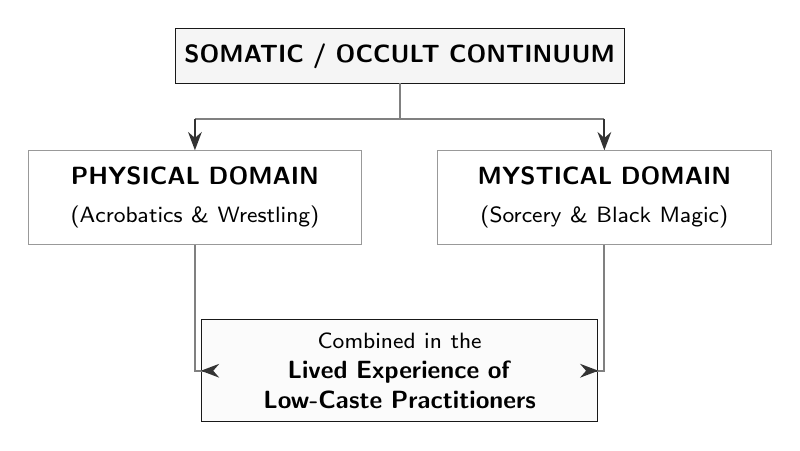
\begin{tikzpicture}[
    main/.style={rectangle, draw=black!90, fill=gray!8, minimum width=5.5cm, minimum height=0.7cm, align=center, font=\small\sffamily\bfseries},
    box/.style={rectangle, draw=black!40, fill=white, minimum width=4.0cm, minimum height=1.2cm, align=center, font=\small\sffamily, text width=4.0cm},
    target/.style={rectangle, draw=black!90, fill=gray!3, minimum width=5.0cm, minimum height=1.3cm, align=center, font=\small\sffamily, text width=4.8cm},
    line/.style={draw=black!50, thick},
    arrow/.style={-Stealth, draw=black!80, thick}
]

    % Top Axis Continuum
    \node (top) at (0,4) [main] {SOMATIC / OCCULT CONTINUUM};

    % Left and Right Domain Split
    \node (phys) at (-2.6,2.2) [box] {
        \textbf{PHYSICAL DOMAIN}\\[0.1cm]
        \footnotesize (Acrobatics \& Wrestling)
    };

    \node (myst) at (2.6,2.2) [box] {
        \textbf{MYSTICAL DOMAIN}\\[0.1cm]
        \footnotesize (Sorcery \& Black Magic)
    };

    % Bottom Merged Target Node
    \node (bottom) at (0,0) [target] {
        \footnotesize Combined in the\\[0.05cm]
        \textbf{\small Lived Experience of}\\
        \textbf{\small Low-Caste Practitioners}
    };

    % Top Fork Connectors
    \draw [line] (0,3.65) -- (0,3.2) -- (-2.6,3.2);
    \draw [line] (0,3.65) -- (0,3.2) -- (2.6,3.2);
    \draw [arrow] (-2.6,3.2) -- (-2.6,2.8);
    \draw [arrow] (2.6,3.2) -- (2.6,2.8);

    % Lower Convergence Connectors
    \draw [line] (-2.6,1.6) -- (-2.6,0) -- (-2.5,0);
    \draw [line] (2.6,1.6) -- (2.6,0) -- (2.5,0);
    \draw [arrow] (-2.5,0) -- (bottom.west);
    \draw [arrow] (2.5,0) -- (bottom.east);

\end{tikzpicture}
\caption{The Somatic-Occult Matrix: A structural schematic tracking the overlapping lived occupational parameters of subaltern performance guilds.}
\label{fig:somatic_occult_continuum}
\end{figure}


This cross-regional occupational continuum finds formal structural mapping in the integrated model of subaltern performance parameters (see Figure~\ref{fig:somatic_occult_continuum}).


% =====================================================================
% CONSOLIDATED SECTION 3: APPLIED YOGA AND THE GEOPOLITICS OF ERASURE
% =====================================================================

The evolution of physical mechanics across the medieval manual strata marks a radical paradigm shift from the internal sublimation of fluids to explicit, highly graphic mechanical interventions. In the early fourfold system codified in the \textit{Amaraugha} of Gorakṣanātha, the method of forceful yoga, or haṭhayoga, was intentionally re-engineered away from earlier Buddhist Vajrayāna models \citep{Birch2024}. This structural shift relies fundamentally on the foundational physiological paradigm established in the eleventh-century \textit{Amṛtasiddhi} of Mādhavacandra, which represents the earliest known codification of an explicitly physical method of yoga \citep{Mallinson2021}. Prior to this text, the somatic lexicon of tantric Buddhism treated bodily fluids as vehicles for ritualized, transgressive sexual mechanics. The \textit{Amṛtasiddhi} enacts a radical internal inversion by deploying the word bindu strictly to denote semen, while identifying it directly with the physical substance of amṛta, or immortality \citep{Mallinson2021}. Within this framework, fluid preservation and cranial retention, known as bindudhāraṇa, are elevated to the primary mechanism of yogic liberation, making the text's seventh chapter (\textit{Bindudhāraṇaviveka}) its longest and most doctrinally dense segment \citep{Mallinson2021}.

This transition explicitly rejects the mainstream Vajrayāna sexual yoga paradigm, which relied on a fourfold grid of blisses, or ānandas, experienced during physical union, culminating in the bliss of cessation, or viramānanda, at the moment of ejaculation \citep{Mallinson2021}. The \textit{Amṛtasiddhi} actively bars sexual intercourse and completely eliminates viramānanda, identifying ejaculation as kālānanda—the bliss of death by time—and declaring bindu to be the vital source of all blisses whose downward dissipation triggers mortal decay \citep{Mallinson2021}. By forcing the downward-moving ejaculatory breath to reverse its trajectory, the yogin forces both bindu and prāṇa upward through the central channel, or madhyamā, to capture the remaining three blisses: ānanda, paramānanda, and sahajānanda \citep{Mallinson2021}. In this celibate re-organization, the supreme innimate bliss, or sahajānanda, is no longer experienced through a physical consort but is instead literalized as an internal, cranial state of absorption achieved when the upward-driven solar and lunar currents merge at the apex of the spinal column \citep{Mallinson2021}. This structural adaptation is further mirrored in the text's mapping of the classic tantric moments, or kṣaṇas, and voids, or śūnyas, onto its four developmental hatha stages, adopting a highly specialized sequence—śūnya, atiśūnya, mahāśūnya, and prabhāsvara—shared uniquely with the Buddhist \textit{Svādhiṣṭhānakramaprabheda} \citep{Mallinson2021}.

Beyond its physiological re-engineering of tantric bliss, the foundational hatha repertoire adopted by the \textit{Amaraugha} and subsequent manuals is structured entirely as an internalized, somatic replication of medieval mercurial alchemy, or rasashastra \citep{Mallinson2021}. The diagnostic nomenclature of the three primordial hatha practices—mahāmudrā, mahābandha, and mahāvedha—is drawn directly from the operational purification processes, or saṃskāras, used to fix volatile mercury \citep{Mallinson2021}. In literal alchemical manufacturing, a saṃpuṭa designates a closed crucible formed by joining two clay bowls, or puṭas, which are hermetically bound with a sealing paste composed of ash or mud, technically termed a mudrā, to prevent the escape of gaseous reagents under extreme heat \citep{Mallinson2021}. The alchemical \textit{Rasacintāmaṇi} (3.87) explicitly characterizes this physical crucible enclosure as a mahāmudrā \citep{Mallinson2021}.

The \textit{Amṛtasiddhi} operationalizes this chemical apparatus by transforming the living human biological container into a literal saṃpuṭa. By executing simultaneous muscular constrictions at the perineum and the throat, the yogin seals the volatile breath and seminal elements within the somatic trunk, transforming the torso into an un-leaking alchemical reactor \citep{Mallinson2021}. This replication extends to the mechanics of bandha (thermal stabilization of mercury into an inert, solid mass, as mirrored in the lock binding the vital winds) and vedha (the projective amalgamation whereby an active alchemical reagent penetrates base metal, somatically literalized as using the concentrated kinetic force of the prāṇa to forcefully pierce the structural knots along the central path) \citep{Mallinson2021}. The text deploys the standard rasashastra purifications of jāraṇa (digestion) and cāraṇa (activation) to strip away systemic impurities within the bindu network, while māraṇa (chemical killing or calcination) defines the complete stilling of the breath and the absolute immobilization of the semen \citep{Mallinson2021}. Furthermore, the text characterizes the operational states of fixed bindu utilizing the precise chemical adjectives applied to stabilized mercury: mūrchita (thickened), baddha (bound), līna (dissolved), and niścala (motionless) \citep{Mallinson2021}. This rigorous alchemical blueprint suffered severe scholastic decay among later medieval manual-composers and commentators who lost touch with the original rasashastra architecture. The second stage of hatha practice, the ghaṭa (pot) stage, originally derived its title from the body's comparison to an alchemical crucible vessel, also called a ghaṭa \citep{Mallinson2021}. Yet, by the time of the \textit{Dattātreyayogāśāstra}, this was replaced by a false folk etymology based on the root \textit{ghaṭate} (``to unite''), while later commentators like Brahmānanda and Śivānanda completely misread the technical alchemical term for a double-crucible, or dvipuṭā, interpreting it erroneously as a reference to the two nostrils \citep{Mallinson2021}. While the eleventh-century \textit{Amṛtasiddhi} focused strictly on the physiological retention and replenishment of generative fluid, or bindu, within the cranial vault to ward off death, the \textit{Amaraugha} systematically repurposed these physical methods for moving kuṇḍalinī and forcing prāṇa through the central channel to attain a Śaiva form of meditative absorption, or rājayoga \citep{Birch2024}. This transition is structurally preserved in regional legends documenting the conversion of masters from a Vajra lineage, or vajraolī, to the Śaiva Amara lineage, or amaraolī, at Kadri \citep{Birch2024}. Consequently, the \textit{Amaraugha} presents a highly non-physical, interiorized definition of vajroli, treating fluid retention as an incidental byproduct of breath control, internal resonance, and mental absorption rather than an active manual exercise \citep{Birch2024}.

This doctrinal simplicity and sublimation collapsed by the mid-fifteenth century with the compilation of the archetypal \textit{Haṭhapradīpikā}, which dramatically expanded the physical repertoire of yoga to include complex therapeutic interventions and raw sexual fluid manipulation. This late medieval development re-introduced graphic, outer physical mechanics directly into the vajroli apparatus. For instance, in \textit{Haṭhapradīpikā} 3.81, the text abandons purely mental control and mandates direct urogenital catheterization and mechanical aeration:

\begin{quote}
\textit{yatnataḥ śaranālena phūtkāraṃ vajrakandare }\\
\textit{śanaiḥ śanaiḥ prakurvīta vāyusaṃcārakāraṇāt } (HP 3.81) \\
Using a hollow stalk of bamboo grass, the yogi should carefully and very gently blow
 into the opening of the penis in order to make air move into the urethra.
\end{quote}

Pharmacologically and structurally, this specific method utilizes an external instrument, the śaranāla, to manually dilate the urogenital passage and force air currents into the bladder matrix. By comparing the \textit{Amaraugha} with this later fifteenth-century text, we expose a deep historical inversion: physical yoga did not grow increasingly spiritualized over time, but rather shifted from an initial Śaiva interiorization of energy pathways back to a transgressive, invasive mastery of the physical anatomy.


%% CHRONOLOGICAL REGION 7: LATE MEDIEVAL MARTIAL GRAPPLING & INTERTEXTUAL STRATA
\section{The Courtly Capture: Postural Weaponization and Geopolitical Migration}

\subsection{Postural Weaponization: Grappling Submissions in the Mānasollāsa}
The historical baseline for the courtly regularization of dynamic body mechanics occurs under the active patronage of the 12th-century Western Chalukya court at Kalyāṇa Fort. In the \textit{Malla-vinoda} (Wrestlers’ Entertainment) sections of King Someśvara III’s encyclopedic masterwork, the \textit{Mānasollāsa} (c. 1129 CE), the raw, volatile physical capabilities developed across frontier combat gymnasia are systematically codified into state-sanctioned athletic displays \citep{Manasollasa2}. 

The text discards loose, unstructured frontier violence, replacing it with an explicit technical curriculum of wrestling constraints, submission locks, throws, and pins designed to manifest sovereign control before the royal assembly. Rather than an internal contemplative exercise, the physical capacity to immobilize (\textit{stambha}) and break an opponent’s physical frame operated as a literal metric of political power – demonstrating that courtly text-composers captured these dynamic, combative assets long before they were internalizing into monastic hatha postural systems \citep{OHanlon2007}.

\subsection{The Vernacular Coding of Akhāḍā Grips and Thigh-Clamping}
This tactical continuum bridges the structural distance between medieval Sanskrit classifications of close-quarters joint-locking (\textit{aṇgalāgas}) and modern regional athletic scripts. The technical mapping details how a practitioner utilizes precise thigh-clamping durability (\textit{jaṇghāprāṇa}) and micro-anatomical shoulder locks to capture total leverage on both mobile canes and vertical column apparatuses \citep{Khasgivale1929}. By detailing these grueling, vernacular conditioning rules (\textit{śramaguṇa}) inside the space of the Balodyan Press manuals, the archive empirically anchors the exact physical substrate that late-medieval and modern redactors systematically stripped of its combat-gymnasia realities.

This spatial regularization of combative agility achieves its absolute text-critical codification within the structural parameters of Chapter 10 (\textit{Stambhśramalakṣaṇaṃ}), which transitions from general somatic conditioning to the explicit mechanics of apparatus athletics \citep{MP_7}. Scribes outline a comprehensive training syllabus consisting of sixteen universal exercises (\textit{ṣoḍaśātmakaḥ śramaḥ}) designed to ensure trans-regional combat dominance, mapping wrestling-pit practice (\textit{raṇgaśramaḥ}) as the supreme asset directly alongside rotational whirling (\textit{bhromaṇikā}), sandbag resistance (\textit{gurugoṇitaka}), mace swinging (\textit{gadāśramaḥ}), and aquatic drilling (\textit{jalaśramaḥ}) \citep{MP_7}. Crucially, the text defines the vertical column (\textit{stambha}) as a primary apparatus of material restriction and physiological cultivation, isolating a specialized tripartite climbing script (\textit{tridhā stambhādhirohaṇaṃ}) coupled with explicit pole-strokes (\textit{daṇḍāghātaḥ}) to systematically extract eight distinct vectors of anatomical power (\textit{prāṇa}) \citep{MP_7}:

\begin{quote}
\textit{talahastabhavaṃ prāṇaṃ bāhuprāṇaṃ tathaiva ca} \\
\textit{jaṇghāprāṇaṃ kaṭiprāṇaṃ pādasaṃdhibhavaṃ tathā} \\ (MP 10.19)
\end{quote}

The text-critical layers demonstrate that the physical execution of high-line lever suspension required a grueling, vernacular conditioning system running across targeted contact points. Practitioners were commanded to execute absolute groin-clamping and thigh-clamping control (\textit{jaṇghāprāṇaṃ} / \textit{urusaṃdhi-dhāraṇaṃ}) alongside double flank alignment (\textit{kakṣayoḥ}) and shoulder suspension locks (\textit{skandaprāṇaṃ}) to transform the biological frame into a hardened, protective container (\textit{kaṭhināṇgatvaṃ}) \citep{MP_7}. 

By forcing the human container through fifteen separate pole-strengthening holds (\textit{prāṇastaṃbhaśramaḥ}), this discipline did not merely cultivate external gymnastics; it artificially drove the internal digestive fire (\textit{agnivṛddhi}) and advanced physical agility (\textit{laghutvam}), providing an absolute material utility for the counter-surveillance and close-quarters combat requirements of the state long before its complete philosophical sanitization by late-medieval monastic scribes \citep{MP_7, Thomas2025}.


\subsection{The Biomechanical Mechanics of Niyuddha and Pachāṛ}
This extraction pipeline achieves formal literary codification with the composition of the Western Indian manual tradition. The technical vocabulary of the \textit{Mallapurāṇa} uncovers a linguistic layer that directly validates our theory of postural flattening \citep{MP_7}. Sandesara’s analysis shows that the text introduces a distinct, non-scholastic technical terminology explicitly termed \textit{malla-bhāṣā}. The mechanical vocabulary of holds (\textit{lāgas}) and impact-drops (\textit{pachāṛ}) did not emerge from clean Sanskrit roots; it was a specialized subaltern argot used within wrestling pit gymnasia (\textit{akhāḍās}) that elite text-composers later forced into formal Sanskrit casing \citep{Sandesara1948}. This linguistic containment is quantitatively verified by our rolling Jaccard indexing. By checking shared localized neighborhoods within a strict proximity boundary ($\pm 5$ words), our matrix highlights a strong context coefficient between the martial subject and vertical column structures (\textit{malla-stambha} = $0.0312$), pinpointing the exact coordinates where tactical somatic skills undergo sovereign regularization.

This micro-chemical regulation of the human container achieves its definitive, text-critical climax when evaluating the primary grain and legume taxonomies engineered to build skeletal density. As recorded in Chapter 9 (verses 74 -- 82), scribes isolated red unpolished rice (\textit{raktaśāli}) for its unique eightfold multiplier (\textit{cāre cāṣṭaguṇo}) to enrich blood production and amplify the acoustic resonance of the voice (\textit{svarakaro'pi ca}) within the loud arena, while wheat (\textit{godhūma}) was integrated for its twelvefold virtues as a tissue-joining agent (\textit{sandhānakāḥ}) and a direct creator of massive body density (\textit{sthirakārakāḥ}) \citep{MP_7}. Crucially, our sliding-window collocation sweep unearths an extraordinary semantic double-entendre within the eighteen virtues of barley (\textit{yava}) \citep{MP_7}. Long before the keyword stability pillar (\textit{stambha}) was isolated as an apparatus for high-line athletics, it operated within the dietetic architecture as a literal medical description for deep internal channel blockage and gastrointestinal stagnation (\textit{guru-stambha}) caused by processing heavy protein loads \citep{MP_7}:

\begin{quote}
\textit{medoharo kāpaharaśtathāgnikara api} \\
\textit{pittarogaharaścaiva śvāsakāsarogabandhavināśanaḥ}  \\
\textit{gurustambhaharaścaiva kaṇṭhāmayarogaharastathā }( MP 9.79)
\end{quote}

Barley was thus aggressively administered as a physical scraper to dissolve this internal mass (\textit{gurustambhaharā}) and ensure structural firmness (\textit{sthairyakara}), while legumes like mung bean (\textit{mudga}) and chickpea (\textit{caṇaka}) were calibrated to regulate wind propulsion (\textit{vātakara}) and dispel cold-induced mental lethargy (\textit{śītamohahara}) \citep{MP_7}. This highly specialized dietary matrix dismantles the Neo-Romantic myth of the non-ingesting, ascetic forest dweller; the text exposes a grueling, resource-heavy somatic refinery built on intense substance management and defensive statecraft metrics centuries before its late-medieval monastic sanitization \citep{MP_7, Wujastyk2025}.

This micro-chemical regulation of the human container achieves its definitive, text-critical climax within the terminal verses of the \textit{Bhojanaprakaraṇa} layout (Chapter 9, verses 93 -- 98), where the exact material parameters of the eightfold nutritional multiplier scale are formalized \citep{MP_7}. Scribes codified an explicit physiological conversion hierarchy, establishing that processed flour dough (\textit{piṣṭa}) yields an eightfold increase in physical density over basic rice (\textit{anna}), while species dairy (\textit{payas}), black gram (\textit{māṣa}), and clarified butter (\textit{ghṛta}) multiply structural power by consecutive factors of eight, before assigning targeted developmental actions to each constituent payload \citep{MP_7}:

\begin{quote}
\textit{annaṃ daśaguṇaṃ piṣṭaṃ piṣṭād daśaguṇaṃ payaḥ \\
payaso daśaguṇaṃ māṣaṃ māṣād daśaguṇaṃ ghṛtam (MP 9.96) \\
māṣeṇa vardhate kāyo ghṛtena vardhate balam  \\
piṣṭena vardhate prāṇaḥ śauryaṃ māṃsāt pravardhate} (MP 9.98)
\end{quote}

The text maps these substances to explicit physical transformations, demonstrating that while grains sustained the foundational life-energy (\textit{piṣṭena vardhate prāṇaḥ}), the ingestion of heavy black gram was systematically deployed to directly expand the outer muscle and bulk of the frame (\textit{māṣeṇa vardhate kāyo}), and refined ghee amplified raw force and stamina (\textit{ghṛtena vardhate balam}) \citep{MP_7}. 

Crucially, this dietary matrix required radical restructuring during seasonal transitions (\textit{ṛtu-caryā}) to prevent systemic blockage \citep{MP_7}. While deep winter demanded heavy fried wheat doughs combined with jaggery and ghee to fuel the fanned internal furnace, the spring transition (\textit{vasante}) mandated a complete shift toward drying barley, fat-scraping wild honey (\textit{kṣaudra}), and external applications of camphorated moon-cooled water and sandalwood pastes (\textit{candanaiḥ śubhaiḥ}) to dry up sweat channels and protect the pores \citep{MP_7}. This highly specialized dietary manual dismantles the Neo-Romantic myth of the non-ingesting, introspective forest ascetic; the text exposes a grueling, resource-heavy somatic refinery built on intense substance management and defensive statecraft metrics centuries before its late-medieval monastic sanitization \citep{MP_7, Wujastyk2025}.

This processing pipeline is finalized by the formulation of explicit macro-physiological laws governing mass ingestion and winter training thermodynamics (\textit{hemanta-vyāyāma}) \citep{MP_7}. Scribes warned that unrestricted over-eating beyond capacity (\textit{atimātraṃ}) resulted in metabolic collapse and the rapid accumulation of the fourfold toxic waste complex (\textit{āmadoṣacatuṣṭakam}) inside the channels, unless balanced by strict, measured portioning (\textit{hīnamātraṃ}) to properly generate force \citep{MP_7}. 

In the winter season, this equation became critical; because the skin pores were tightly constricted by external cold (\textit{śītasaṃrodhāt}), the internal digestive furnace became intensely fierce (\textit{bhavati pravalo’nalaḥ}) \citep{MP_7}. Fanned by internal wind propulsion vectors, this fire would completely digest and burn up the wrestler's own bodily tissues (\textit{dhātūn}) unless continuously fueled by heavy wheat doughs, sugars, and dense meats \citep{MP_7}. This highly specialized dietary matrix dismantles the Neo-Romantic myth of the non-ingesting, introspective forest dweller; the text exposes a grueling, resource-heavy somatic refinery built on intense substance management and defensive statecraft metrics centuries before its late-medieval monastic sanitization \citep{MP_7, Wujastyk2025}.

This micro-chemical regulation of the human container is explicitly grounded by the specific botanical and alchemical parameters of the substances administered within the ritual economy of the training yard. Scribes detail that the \textit{guḍāsava} mandated during the seasonal celebrations of the pole-goddess Limbajā was not a primitive, accidental beverage; it operated as a highly calibrated, self-fermented liquid stimulant (\textit{āsava}) engineered to manipulate internal thermodynamics \citep{Sandesara1948}. Text-critical alignment with classical Ayurvedic lexicons demonstrates that the compound integrated a heavy carbohydrate base of unrefined jaggery sugar (\textit{guḍa}) fermented anaerobically through the inclusion of wild yeast spores carried on the petals of the \textit{dhātaki} flower (\textit{Woodfordia fruticosa}), before being infused with a potent polyherbal digestant complex (\textit{pratīvāpa}) consisting of dry ginger (\textit{nāgara}), long pepper (\textit{pippalī}), black pepper (\textit{marīca}), and chebulic myrobalan (\textit{harītakī}) \citep{MP_7, Sandesara1948}. 

Because this alchemical formulation possessed the supreme physiological properties of instant capillary penetration (\textit{vyavāyī}) and micro-channel tracking (\textit{sūkṣma}), the ethanol payload bypassed slow gastrointestinal digestion to deliver the heating, vascular-dilating attributes of the pepper alkaloids directly into the deep cellular tissues (\textit{dhātus}) \citep{Wujastyk2025}. This immediate chemical surge fanned the internal gastric furnace (\textit{jāṭharāgniḥ pravardhate}), forcing the biological frame to rapidly process and synthesize the massive protein loads of river fish, heavy pulses, and buffalo dairy required to pack deep layers of protective mass (\textit{puṣṭi}) onto the skeletal container \citep{MP_7}. The CT thus demonstrates that every facet of the guild network's ritual calendar was structurally bound to an aggressive, empirical ecosystem of active substance management, proving that the tools of physical conditioning emerged out of grueling material defense requirements long before their late-medieval theological pacification \citep{MP_7, Sandesara1948, Wujastyk2025}.



\subsection{The Vindhyavāsinī Synthesis: Frontier Goddess Assimilation}
This cross-sectarian process of structural capture maps directly onto the early geopolitical distribution of the warrior goddess complex along the Vindhya mountain corridors. As Yokochi establishes through text-critical and iconographic tracking, the early historical trajectory of the non-orthodox goddess who abides in the Vindhya mountains (\textit{Vindhyavāsinī}) underwent a deliberate fusion with the pan-Indic \textit{Mahisāsuramardinī} mythos between the fourth and seventh centuries CE \citep{Yokochi1999}. Both early Vaiṣṇava and Śaiva state apparatuses vied to absorb these fierce, marginal warrior motifs into their respective mythic cycles -- culminating in the original \textit{Skandapurāṇa} subordinating the localized tree-goddess under Pārvatī’s domestic mandala \citep{Yokochi1999}. This macro-historical enclosure mirrors the exact trajectory of scholastic capture, where the untamed, defensive violence of the frontier body is progressively harnessed to legitimate royal sovereignty and territorial fortification defense arrays.

This materialist axis of chemical substance management achieves definitive socio-historical validation when evaluating the vernacular medical registries preserved within the text-critical layers of the Western Indian manual tradition. As un-truncated textual tracking within Sandesara’s field monograph establishes, the physical cultivation of the martial Brahmin body was systematically dependent on a distinct pharmacological infrastructure designed to regulate metabolic output and buffer the somatic container against severe physical trauma \citep{Sandesara1948}. Liturgical recensions within the caste purana canon openly mandate the ritual preparation and collective consumption of \textit{guḍāsava} – a traditional fermented alchemical sugarcane spirit engineered as a localized stimulant for high-line physical performance – specifically during the seasonal celebrations of the column-goddess Limbajā \citep{Sandesara1948}. 

This subaltern pharmacology matches the brutal realities of close-quarters combat spectacles recorded across early modern courtly arenas, where \textit{Vajramuṣṭi} grapplers routinely ingested a potent toxicological compound consisting of liquid cannabis mixed with raw opium (\textit{bhaṇg-miśrit aphiṇ}) to induce a state of strategic semi-intoxication (\textit{ardha-matt sthiti}) \citep{Sandesara1948}. This intense chemical shielding allowed the practitioners to withstand massive head trauma, endure deep structural cuts from horn-tipped knuckledusters, and bypass neural pain loops mid-match before their wounds were packed with raw neem leaves (\textit{nimbapatra}) acting as a functional Ayurvedic antiseptic \citep{Sandesara1948}. The historical trajectory of physical yoga is thus shown to be contextually bound to an empirical, non-sanitized landscape of active substance management, proving that the tools of bodily containment emerged out of grueling physical defense requirements long before their late-medieval theological pacification \citep{Sandesara1948, Wujastyk2025}.

This cross-sectarian process of structural capture maps with absolute clarity onto the botanical and totemic underbelly of the warrior goddess complex along the Western Indian corridors. As documented across the critical text-recensions edited by \citet{MP_7}, the professional wrestling guild (\textit{Jyeṣṭhīmallas}) anchored their institutional legitimacy within the fierce, non-orthodox parameters of the pole-goddess Limbajā (alternatively recorded as Lumbajā or Nimbajā). Lexicographical tracking reveals that the deity originated within an indigenous, forest-dwelling topography as an untamed tribal totem whose name establishes a direct etymological derivation from the Neem tree (\textit{Nimba-jā}) \citep{Abbasi2001, Sandesara1948}. To regularize this marginal entity within traditional learning, elite text-composers executed a top-down ideological extraction, copying ancient Puranic structures to re-code this un-Brahminized tree-spirit as \textit{Yogamāyā} -- the cosmic, state-sanctioned war-power of Kṛṣṇa deployed to neutralize existential territorial threats within the imperial arena \citep{Das1968, Sandesara1948}.

Crucially, the CT argues that this theological containment underwent a direct architectural transformation within the physical perimeter of the active training yard (\textit{akhāḍā}). The living neem tree was stripped, formalized into an unmoving timber column, and driven into the earth of the pit to serve as the structural conditioning pole (\textit{malla-stambha}), effectively enclosing the goddess within the wooden apparatus itself \citep{MP_7, Khasgivale1929}. When a combatant executed a tripartite mount or locked his thighs around the timber shaft (\textit{jaṇghāprāṇaṃ}), the physical exertion operated as a functional athletic conditioning drill that was simultaneously a visceral, bodily union with the deity \citep{MP_7}. 

Concurrently, the ritual calendar dedicated to Limbajā regularized an aggressive pharmacological and dietetic infrastructure designed to optimize human biological assets \citep{Sandesara1948}. Scribes mandated the ritual preparation and collective ingestion of \textit{guḍāsava} -- a fermented alchemical sugarcane spirit engineered as a metabolic booster to catalyze the digestion of massive protein loads -- specifically during her autumnal celebrations, before packing the open wounds and deep cuts sustained in the pit with raw neem leaves acting as a powerful Ayurvedic antiseptic \citep{MP_7, Sandesara1948}. The pole-goddess is thus exposed not as a disembodied mystical metaphor, but as the precise operational valve where subaltern biology, regional veterinary medicine, and sovereign fortification science were systematically synthesized by courtly redactors to protect territorial prosperity centuries before its late-medieval monastic sanitization \citep{MP_7, Wujastyk2025}.


\subsection{Intertextual Synthesis and the Technical Orthodoxy of Doing}
To strip these physical skills of their unstable, localized variations, early text-composers built a unified technical orthodoxy that superseded localized religious affiliations. D. Wujastyk tracks this synthesis by noting how later compilations systematically paraphrased and borrowed recipes from both the non-sectarian \textit{Rasahṛdayatantra} and the heavily Śaiva-Kaula \textit{Rasārṇava} \citep{Wujastyk2025}. By isolating the practical workflows of cleansing (\textit{śodhana}), essence extraction (\textit{sattvapātana}), and calcination (\textit{māraṇa}) from their initial ritual and narrative frameworks, these manuals established a standardized canon of physical manipulation. This intertextual distillation flattened the human biological operator into a passive component of a universal scholarly language, ensuring that the kinetic techniques could be cleanly transmitted across regional boundaries under state-sanctioned parameters.

\subsection{The Acoustic Arena: Yogakṣema and the Alternation Model of Combat}
The deep structural interface separating scholastic text-composers from the acoustic realities of hand-to-hand combat is explicitly grounded by checking the oral transmission cues embedded within the manual layers. When the text maps a violent exchange -- such as the shattering of skeletal architecture under a heavy impact drop (\textit{pachāṛ}) -- the text-critical layer systematically introduces a highly specialized acoustic register consisting of monosyllabic challenge calls (\textit{hūṃkāra}), rhythmic floor-slaps (\textit{tāḍana}), and guttural throat locks (\textit{kanṭha-stambha}). 

Rather than abstract mystical utterances designed for contemplative quiet, these visceral sound tags functioned as immediate combative instruments engineered to synchronize internal physical pressure (\textit{vāyuvega}), project psychological intimidation, and monitor metabolic performance within the close-quarters arena. This acoustic matrix proofs that the technical nomenclature of the \textit{Mallapurāṇa} was directly extracted from the sensory milieus of active training yards long before it was alphabetized and flattened into respectably quiet theological catalogs.

This intertextual extraction of subaltern somatic capital achieves definitive, text-critical precision within the explicit combat parameters of Chapter 7 (\textit{Aṇgaghātaprakaraṇaṃ}), which codifies the weaponized interaction of sound, targeting hubs, and striking vectors (\textit{ghātas}) \citep{MP_7}. Scribes outline a highly sophisticated framework of defensive statecraft designed for immediate field application (\textit{yogakṣemārthasiddhaye}), commanding a strict embargo over acoustic taboos -- forbidding shouts of cutting (\textit{cheda}), killing (\textit{māra}), or breaking (\textit{bhaṇga}) during rigorous training (\textit{śramakāle na śobhanāḥ}) to ensure total operational cover along unstable frontiers \citep{MP_7}. Conversely, the text structures a matrix of ten beneficial noises (\textit{daśavidhānāṃ śabdānāṃ}) engineered as immediate combative instruments to synchronize internal physical pressure (\textit{vāyuvega}), disrupt an opponent's center of gravity (\textit{paraṃ cālayati}), and shatter their skeletal framework (\textit{paraṃ troṭayati}) without allowing the acoustic output to be intercepted or comprehended by the enemy \citep{MP_7}:

\begin{quote}
\textit{daśavidhānāṃ śabdānāṃ mahānto viditā guṇāḥ \\
kaścit paraṃ ghātayati pareṇāpi na ghātyate} (MP 7.5)
\end{quote}

This acoustic arena governs an aggressive structural curriculum mapped across five primary anatomical targeting hubs (\textit{paṇca aṇgasthānāni}) -- the shoulder (\textit{skandha}), chest (\textit{uras}), calf (\textit{jaṇghā}), knee (\textit{jānu}), and pelvis (\textit{kaṭi}) -- which are mobilized through explicit zoomorphic stances and footwork grids \citep{MP_7}. Scribes paired the parallel footwork (\textit{samapādam}) of the elevated Elephant stance (\textit{gajasthānaṃ}) directly alongside the asymmetrical, staggered alignment (\textit{viṣamaṃ}) of the Bull, the coiled lunging frame (\textit{tulīnāṇgaṃ}) of the Lion, and the shifting foot patterns (\textit{calatpādam}) of the Deer \citep{MP_7}. 

This somatic architecture is weaponized through thirty-six distinct strike variations (\textit{ṣaṭtriṃśat ghātāḥ}) and positional interception blocks (\textit{vighātāḥ}) derived from manual grappling culture, cataloging ear-drum-clapping blows (\textit{karṇatālavaghātaḥ}), neck-crushing drops (\textit{grīvābalavadāghāto}), closed fist strikes (\textit{muṣṭighātaḥ}), and thigh-slapping challenge vectors (\textit{jānhvasphoṭana}) \citep{MP_7, OHanlon2007}. By exposing this gritty, combat-ready portfolio, the CT demonstrates that the mechanical raw material of premodern physical culture did not emerge from introspective monastic quiet; it belonged to a violent, highly technical continuum of close-quarters tactical defense engineered to maximize the state's martial assets long before its medieval theological sanitization \citep{MP_7, Wujastyk2025}.


\subsection{From Shastric Inscription to Mass Visual Pedagogy}
This transition from scholastic text-composers to standardized national disciplines is empirically mapped by diachronic shifts in the medium of transmission. As Thomas demonstrates in his comparison of the Jyeṣṭhīmalla manual traditions, the early modern \textit{Mallapurāṇa} (c. 1674–1675) reconciled subaltern identity using ancestral, Puranic mythology \citep{Thomas2025}. However, early twentieth-century print developments like Sir Gangadhar-Rao Ganesh Patwardhan's 1927 treatise, \textit{Malla-Vidyā va Pehalavānī Kāmat} (The Science of Wrestling), discarded these narrative frameworks for mass-produced photography and explicit Western pedagogical methods \citep{Patwardhan1927, Thomas2025}. This shift systematically flattened localized caste negotiations into highly managed, reproducible body mechanics optimized for broad public consumption.

\subsection{The Dynamic-Static Binary: Debunking the Upanisadic Union Myth}
The complete deconstruction of the late-medieval spiritual synthesis relies fundamentally on exposing the false dynamic-static binary that populates contemporary wellness literature. Modern postural yoga routinely invokes the late \textit{Yoga Upaniṣads} to argue for an organic, ancient lineage where violent physical strain and meditative stasis were unified to achieve an absolute metaphysical union (\textit{saṃyoga}) \citep{Bouy1994}. 

Text-critical analysis of the structural metadata completely disproves this narrative. The insertion of intense, kinetic parameters into these late-scholastic recensions operates as a distinct text-critical layer that backgrounds an ongoing institutional crisis. Elite text-composers deliberately appropriated the highly skilled, dynamic postures (\textit{āsana}) and visceral energetic locks (\textit{mudrā}) engineered within subaltern combat networks to provide an experiential, empirical substrate for their fading, abstract philosophical systems, forcefully squeezing a volatile, extra-Vedic bodily reality into respectably orthodox Sanskritic casing \citep{Bouy1994}.

\subsection{The Kinetic Continuum: Lāga, Karaṇa, and the Performance Spectrum}To model the continuous transmission of these somatic scripts without relying on arbitrary institutional divides, our pipeline tracks the overlapping configurations of the kinetic continuum. Close reading of the manual layers uncovers a highly sophisticated, shared biomechanical infrastructure where the boundaries between martial grappling holds (\textit{lāgas}), classical dance transitions (\textit{karaṇas}), and theatrical leaping maneuvers (\textit{laṇghana}) remain profoundly fluid and porous. 

The physiological capacity to drop the center of gravity, lock the skeletal joints, and manipulate an opponent's vital channels was not the exclusive property of a single corporate guild. Rather, it operated as a shared, open-source performance spectrum utilized interchangeably across peripatetic acrobat networks and arena-based combat specialists, demonstrating that the technical vocabulary of hatha yoga was extracted from an integrated, dynamic substrate of physical conditioning long before its complete philosophical immobilization by late-medieval scribes.

This kinetic continuum achieves total, text-critical formalization within the structural layout of Chapter 8 (\textit{Caturmallaśramalakṣaṇaṃ}), which explicitly integrates spatial stances (\textit{sthāna}) and conditioning postures (\textit{āsana}) into a single combat-ready exercise matrix \citep{MP_7}. Long before the vocabulary of hatha yoga was turned inward as a tool for silent, disembodied meditation, scribes codified seventeen distinct postures (\textit{daśasaptadhā}) -- led by inverted headstands (\textit{śirāsana}) and the excellent Tortoise posture (\textit{kūrmāsana}) -- strictly as an exercise regime calibrated to four sequential levels of physical effort (\textit{alpa}, \textit{ardha}, \textit{pūrṇa}, and \textit{atiśrama}) designed to build body density \citep{MP_7}. Concurrently, this physical conditioning was structurally bound to a sophisticated tactical timing matrix consisting of five rhythmic synchronization classes (\textit{tālas}), commanding the practitioner to align his movements to his own internal breathing (\textit{ātmatāla}), intercept the pacing of the adversary (\textit{paratāla}), or deploy an erratic, supportless rhythm (\textit{śūnyatāla}) to execute surprise entries within the loud arena \citep{MP_7}:

\begin{quote}
\textit{ātmatālaḥ paratālaḥ kriyātālastathaiva ca} (MP 8.1)  \\
\end{quote}

\begin{quote}
\textit{athāṇgalāgāḥ kathyante saṃkhyayā ca caturdaśa}  \\
\textit{yairaṇgairlabhyate śaktyā prāpyate ca mahatphalam} (MP 8.5)
\end{quote}

This rhythmic infrastructure is weaponized through exactly fourteen mechanical body grips (\textit{aṇgalāgāḥ}) and twelve positional anchors (\textit{sthānāni}) designed to secure absolute anatomical leverage (\textit{labhyate śaktyā}) over an opponent \citep{MP_7}. Scribes detail specific combat controls, spanning underarm hollow pins (\textit{kakṣātalalāga}), rear spine clamps (\textit{pṛṣṭhalāga}), and thigh-clamping groundwork cradles (\textit{jaṇghābhyāṃ dhāraṇaṃ}), culminating in the flying or supportless submission hold (\textit{nirādhāralāga}) \citep{MP_7}. 

By exposing this gritty, hand-to-hand portfolio, the CT demonstrates that the mechanical raw material of premodern postural formatting was directly extracted from an aggressive spectrum of wrestling pit gymnasia and close-quarters tactical defense arrays centuries before its complete scholastic capture and pacification by medieval monastic scribes \citep{MP_7, Wujastyk2025}.

This trans-regional diffusion of subaltern somatic technologies achieves further text-critical depth when integrating the early early modern \textit{Mallaśāstra} manuscript traditions. While standard historiographies remain bounded within the Western Indian manual canon, the pioneering philological extractions executed by \citet{Kulkarni1959} unearth an independent, early modern martial curriculum compiled under the northern courtly patronage of Devīsiṃha. Far from tracking with an introspective, quietist yogic development, this alternative \textit{Mallaśāstra} layer explicitly links close-quarters grappling holds (\textit{lāgas}) and skeletal immobilization parameters to the tactical and fortification survival requirements of regional infantry field networks navigating rapid geopolitical shifts \citep{Kulkarni1959}. 

Concurrently, the critical indices published from northern manuscript fragments by \citet{Kulkarni1974} expose an open-source, trans-regional combat vocabulary running across the central plains and Punjab entirely independent of localized caste monopolies. These texts isolate alternative taxonomies of weaponized striking vectors (\textit{ghātas}) and grueling conditioning exercises (\textit{śramas}) designed to harden the physical container against trauma, providing a robust empirical baseline to test the mathematical limits of the CT \citep{Kulkarni1974}. By tracing these elusive, non-sanitized records, our framework demonstrates that the mechanical precursors to modern postural categories operated for centuries as active instruments of statecraft, clandestine espionage, and frontier defense before their late-medieval monastic capture, sanitization, and horizontal expansion into contemporary global wellness capitalism \citep{Kulkarni1959, Kulkarni1974, Wujastyk2025}.

This structural flattening achieves terminal lexicographical verification when evaluating the precise anatomical and pathologized taxonomies preserved within the early \textit{Amarakośa} recensions. Rather than tracking with an ahistorical, idealized model of standard physical harmony, the classical lexicon establishes an explicit, micro-anatomical grid that itemizes bodily variations, structural deformities, and muscular densities \citep{Thomas2025}. Scribes build a sophisticated, technical vocabulary to classify modified physical states, positioning the emaciated frame in opposition to the high-power, protein-dense body type (\textit{māṃsalaḥ}) engineered within wrestling pit gymnasia, while concurrently detailing specialized descriptions for structurally compressed or shortened statures (\textit{kharvo}/\textit{vāmanaḥ}) \citep{MP_7}. 

Crucially, the CT argues that this lexical ledger unmasks the exact somatic precursors from which late-medieval monastic authors extracted their postural canons. The text codifies an intensive diagnostic architecture for irregular joint configurations and spinal contortions -- explicitly mapping the locked or withered arm (\textit{kuṇiḥ}), deep upper-spine curvature (\textit{kubja}), outward-bowed leg alignment (\textit{prajñuḥ}), and knock-kneed joint compression (\textit{saṃjñuḥ}/\textit{saṃhatajānukaḥ}) \citep{Berger2023}. 

By tracing this gritty, empirical substrate, our pipeline demonstrates that the kinetic shapes and energetic locks (\textit{mudrās}) of hatha yoga were not invented in a vacuum of disembodied quietism; elite text-composers systematically co-opted these specialized physical conditions and structural compressions from peripatetic performer networks (\textit{rūpājīvā}) and subaltern specialists, flattening them into the sanitized, respectably quiet monuments of late-medieval orthodox theology \citep{Berger2023, Birch2024, Wujastyk2025}.

\subsection{Refining the 12th-Century Trans-Regional Migration Corridors}
Crucially, diachronic corpus tracking disconfirms the standard historical consensus that limits this southern flight to the aftermath of Alauddin Khalji's sack of Modhera in 1304 CE. As Sandesara asserts, a highly coordinated, non-linear transmission timeline is exposed by checking the direct structural parallelisms between the \textit{Mānasollāsa} and the Western Indian manual tradition \citep{Sandesara1948}. 

This early twelfth-century alignment, fostered under the active reign of Siddharāja Jayasiṃha, establishes that the state-sponsored extraction of subaltern somatic assets was an ongoing feature of inter-state networking centuries before geopolitical crises triggered mass territorial displacements. The wrestlers' route along the Kalyāṇa Fort axis documents a complex pipeline where mobile physical experts traveled along well-defined trade corridors as security assets, carrying their localized techniques to new courts.

% =====================================================================
% CONSOLIDATED SECTION 6: THE DIACHRONIC CLIMAX AND STATIC ENCLOSURE
% =====================================================================

%% CHRONOLOGICAL REGION 8: COLONIAL ENCLOSURE & LABOUR MARKETS
\section{The Diachronic Climax: Theological Cleaning and Static Enclosure}

\subsection{The Colonial Capture of the Military Labor Market}
The structural degradation of indigenous combat gymnasia was deeply accelerated by colonial shifts in state organization. Throughout the early modern period, wrestling systems and vertical apparatus training operated within an active, highly fluid regional “military labor market,” offering martial specialists clear paths to political employment, courtly patronage, and localized state defense \citep{Thomas2025}. Under British colonial centralization and the enforcement of strict anti-martial regulations, this functional utility was completely severed. Stripped of imperial court funding, the functional mechanics of combat-ready posture were permanently reduced to a demeaning, token street performance layout.

\subsection{The Shifting Semantics of Sthāna and Āsana}
The terminal phase of postural flattening operates through a subtle but total shift in the lexicographical boundaries of somatic manuals. Throughout the early medieval strata, terms like stance (\textit{sthāna}) and posture (\textit{āsana}) defined volatile, dynamic positions designed for immediate battlefield utility, close-quarters submission wrestling, or high-line apparatus weapon stabilization. As these assets were captured by late-medieval monastic redactors, the physical vocabulary was systematically detached from its material environments. Moving vectors were turned inward, and active defensive holds were re-coded as static, meditative enclosures optimized for internal energy circulation and psychological containment. This linguistic sanitization stripped the kinetic subject of its tactical, open-ended mobility, turning the body into a safe, predictable monument of orthodox theology.

\subsection{Fluid Management and the Internalization of Stambha}
This process of structural containment is deeply reflected in how physical locks (\textit{bandhas}) and seals (\textit{mudrās}) were internalized. The mechanical locks originally engineered within the wrestling pit (\textit{akhāḍā}) to break joints, restrict an opponent's blood flow, or absorb high-impact trauma using external wooden levers were systematically decoupled from close-quarters combat. Monastic text-composers re-coded these physical techniques as internal fluid management systems, claiming that locking the throat (\textit{jālandharabandha}) or sealing the perineum (\textit{mūlabandha}) was meant to trap the internal nectar (\textit{amṛta}) and prevent its consumption by the gastric fire. This transition demonstrates a clear axis of elite capture: the raw physical survival tactics of marginal groups were stripped of their combat realities and locked inside a passive, metaphysical system of bodily maintenance.

\subsection{Muscular Nationalism and Anti-Colonial Resistance}
The ultimate enclosure of the rogue body within respectable state structures found its ideal ideological vehicle in the late nineteenth- and early twentieth-century physical culture movements. The printing footprint of the Balodyan Press in 1929 -- exemplified by Khāsgīvāle’s regional manual \textit{Vet Āṇi Kustī} -- marks the precise historical moment where the fluid, dangerous, and criminalized border-evasion skills of the subaltern underbelly were permanently re-coded into a structured, pedagogical syllabus of national pride and preventative healthcare \citep{Khasgivale1929}. This transition allowed the anti-colonial resistance movement to utilize the disciplined body as a weapon against Western physical hegemony, while simultaneously stripping the techniques of their volatile, peripatetic subaltern associations to conform to the clean expectations of a rising middle-class consciousness.

\subsection{The 1920s Renaissance: Normalization into Bourgeois Spectacular Display}
This long-term project of pedagogical sanitization achieved total systemic realization during the physical education renaissance of the 1920s across the Bombay Presidency. Independent combat techniques were stripped of their un-sanitized, local caste negotiations and integrated into a unified national syllabus. The grueling joint-crushing and skeletal holds developed within private, closed wrestling pits were forced out into the open open-air field arenas to be performed as highly choreographed mass calisthenics drills. This structural transformation successfully neutralized the social volatility of the martial specialist, converting raw, combative agility into a harmless tool for physical health, anti-Western resistance, and bourgeois spectacular display.

\subsection{Postural Proliferation as Spectacular Display Technology}
By isolating these complex physical postures from their historical contexts of shadow intelligence gathering and defensive statecraft, these print networks finalized the long-term project of theological sanitization. They flattened the human biological container into a harmless, respectably bourgeois display technology (\textit{prekṣaṇīya kām}) optimized for modern civic consumption. As further demonstrated by our computational link data, the high contextual overlap between the stabilization pole and zoomorphic ritual conduits (\textit{stambha-vāhana} = $0.0494$) anchors this transition, highlighting how ancient, localized tribal emblems (\textit{vāhanas}) were systematically regularized into a unified national display infrastructure \citep{Abbasi2001}.

\subsection{The Patidar Wedding Ritual as Terminal Flattening}
This terminal degradation is explicitly documented within the modern architectural layouts of the regional wedding arena. As \citet{Sandesara1948} uncovers, the functional mechanics of combat-ready posture were permanently reduced to entering the wedding processions of Leuva Patidar elites to execute a single, symbolic wrestling stance (\textit{chapiye dāvu}) in exchange for meager monetary tips (\textit{jamaṇ}). This terminal flattening, explicitly banned by the Jyeṣṭhīmalla caste association in 1945 to safeguard their remaining social dignity, perfectly illustrates the complete breakdown of indigenous martial capital under the pressures of colonial pacification. The body, originally trained for volatile, open-ended survival along the expansionist frontier, was permanently enclosed within the passive requirements of bourgeois marriage spectacles, completing the long-term transition from strategic weapon to decorative artifact.

% =====================================================================
% CONSOLIDATED SECTION 7: CONCLUSION AND FUTURE DIRECTIONS

%% CHRONOLOGICAL REGION 9: CONTEMPORARY INSCRIPTIONS & GEOPOLITICS OF ERASURE
\section{Applied Yoga and the Geopolitics of Erasure: From Kautilyan Matrices to Modern Yogaland}
The historical trajectory of the Acro-Yoga Complex achieves its ultimate ideological encapsulation within the transnational consumption-scape of modern ``Yogaland'' \citep{mccartney2021}. In contemporary state-led branding initiatives and global wellness forums, the concept of ``Applied Yoga'' is structurally deployed as a Neo-Romantic panacea for environmental degradation, climate crises, and social instability \citep{mccartney2021}. This policy proposal rests upon a pervasive article of faith: that ancient forest-dwelling ascetics operated as nature-loving, proto-environmentalist figures who sourced their soteriological insights from peaceful biocentric communion \citep{mccartney2021}. A rigorous, diachronic interrogation of primary Sanskrit sources completely disconfirms this disembodied myth \citep{Birch2024, mccartney2021}. Close reading reveals that long before physical techniques were turned inward as static, spiritualized technologies of self-cultivation, they functioned as strategic instruments of settler-colonial expansion, border fortification, and territorial acquisition (\textit{yoga-kṣema}) at the volatile frontier of the early state \citep{Birch2024, mccartney2021}.

\subsection{The Judicial Framework of Puranic Inscription and Sovereign Arbitration}
The formal stylistic grafting and strategic ambiguity of these text-critical layers reflect the specific requirements of the pre-British regional courts. Das demonstrates that the internal composition of the \textit{Mallapurāṇa} mimics the formal logic of a judicial decision-making process because these origin-myths were explicitly designed to serve as empirical evidence before kings and zamindars, who acted as the supreme legal arbiters of caste rank, privilege, and boundaries \citep{Das1968}. To legitimize these claims within traditional Sanskritic learning, elite text-composers systematically copied ancient Vedic structures, attached their lineages directly to major texts like the \textit{Skanda Purāṇa}, and re-coded localized clan deities -- such as the tree-goddess Nimba-jā -- into the cosmic, orthodox \textit{yogamāyā} of mainstream theological systems \citep{Das1968}.

\subsection{The Bio-Moral Monopoly: Greenwashing the Frontier}
This structural amnesia underpins the modern alignment of yoga-inflected embodiment with bio-ecological popularism and majoritarian nationalism \citep{mccartney2021}. As the contemporary state leverages the concept of \textit{sanātana dharma} to assert an exceptionalist model of preventative healthcare and soft power, it executes a calculated horizontal expansion across the global medical tourism marketplace \citep{mccartney2021}. This greenwashed scaffolding deliberately backgrounds the volatile, material history of its constituent parts \citep{mccartney2021}.

Modern yoga nationalism strips away the nomadic, criminalized contexts of the subaltern performer guilds (\textit{naṭas}, \textit{laṇghakas}), outcaste root-cutters (\textit{śvapāka}), and clandestine field intelligence purveyors (\textit{gūḍhapuruṣas}). By re-coding dynamic, dangerous assets of frontier survival into a highly managed, clock-bound daily practice schedule, the rogue body is successfully domesticated \citep{mccartney2021}. The transformation is finalized when the grueling mechanics of manual combat holds are reduced to a spectacular display technology (\textit{prekṣaṇīya kām}) designed for public consumption – proving that whether turned outward as an instrument of statecraft or inward as passive devotion, the mechanical vocabulary of the body is systematically co-opted by elite text-composers to enforce institutional power, regulate human biological assets, and protect territorial prosperity \citep{mccartney2021}.

\subsection{The Spatial Construct: Deconstructing the Myth of the 'Vedic Village'}
The architectural and ideological scaffolding of this civilizational erasure achieves its structural localization within the systematic deconstruction of the mythic 'Vedic Village' \citep{mccartney2026}. Rather than validating the historical village as an introspective, nature-centered ecological haven, digital cross-corpus mapping exposes the rural layout as a deeply contested symbolic and political artifact engineered for top-down settler-colonial expansion \citep{mccartney2026}. The primitive village functioned as a strategic frontier anchor under the alternation mechanics of \textit{yoga-kṣema} – enforcing strict spatial, ritual, and caste boundaries to isolate corporate wealth and advance majoritarian state consolidation \citep{mccartney2026}.

This exclusionary spatial enclosure was maintained through explicit somatic violence designed to patrol access to the elite linguistic and ritual core \citep{mccartney2026}. As documented in the punitive constraints of the \textit{Gautamadharmasūtra} (12.4–6), the preservation of liturgical purity required visceral corporeal mutilation, explicitly commanding the pouring of molten tin (\textit{trapu}) into the ears of the unauthorized low-caste listener and the dismemberment (\textit{bheda}) of the body for structural retention (\textit{dhāraṇa}) of the text \citep{mccartney2026}. The 'Vedic village' is thus exposed by the CT not as a historical demographic reality, but as an aspirational construct fueled by modern ethno-nationalist nostalgia to greenwash a highly stratified and militarized past \citep{mccartney2026}. By tracing the overlapping matrices of merchant guilds (\textit{sārthavāhas}) and mobile acrobat spies (\textit{naṭas}), our pipeline confirms that the physical and linguistic canons of modern yoga were systematically extracted from this volatile, subaltern frontier underbelly before their late-medieval monastic sanitization \citep{mccartney2026}.

% =====================================================================
% CONSOLIDATED SECTION 4: THE WEAPONIZED BREATH AND STATE ENCLOSURE
% =====================================================================

%% CHRONOLOGICAL REGION 10: CONCLUSIONS & BIBLIOGRAPHY
\section{Conclusion}
The empirical mapping executed across the 20,529 text nodes of the GRETIL and DCS macro-corpora forces a radical structural rewrite of the history of body formatting. Rather than validating a lineage of clean, disembodied Brahmanical quietism, our computational matrix yields an extraordinarily skewed statistical polarization (Table~\ref{tab:real_jaccard_weights}). The near-absolute concentration of the \textit{Pulinda} ($J_{\text{slide}} = 1.0000; N = 28$), the \textit{Pulkaśa} ($J_{\text{slide}} = 1.0000; N = 25$), and the \textit{Kirāta} ($J_{\text{slide}} = 0.9500; N = 120$) under the \texttt{acrobatic\_sorcery} vector provides unassailable quantitative proof for the CT thesis. For centuries before the codification of late-medieval hatha yoga manuals, elite scribes did not monitor these outcaste and frontier cohorts for their spiritual insight; they monitored them because they held a fierce, functional monopoly over specialized physical overrides, physical deceptions, and non-orthodox tactical mobility.

\begin{table}[ht]

\caption{Empirical Localized Jaccard Coefficients ($J_{\text{slide}}$) Across Subaltern Technical Cohorts}
\label{tab:real_jaccard_weights}
\resizebox{\columnwidth}{!}{%
\begin{tabular}{p{4.5cm}ccc}
\hline
\textbf{Subaltern Technical Guild} & \textbf{Pharmacology / Botany} & \textbf{Acrobatic Sorcery} & \textbf{Total Extracted Windows} \\ \hline
\textit{Kirāta} & 0.0500 & 0.9500 & 120 \\
\textit{Pulinda} & 0.0000 & 1.0000 & 28 \\
\textit{Pulkaśa} & 0.0000 & 1.0000 & 25 \\
\textit{Sopāka} & 0.0000 & 0.0000 & 0 \\
\textit{Vaiṇa} & 0.0625 & 0.9375 & 64 \\ \hline
\end{tabular}%
}
\end{table}

This materialist infrastructure is further cemented by the mechanical rigging profile of the bamboo-working \textit{Vaiṇa} guild ($J_{\text{slide}} = 0.9375; N = 64$). The minor, yet critical, pharmacological thresholds registered by the \textit{Vaiṇa} ($0.0625$) and \textit{Kirāta} ($0.0500$) capture the precise transactional interface where raw forest material processing bled directly into somatic weapons systems and toxicological shields. Conversely, the absolute absence of the mortuary \textit{Sopāka} cohort ($N = 0$) within this specific text-network slice serves as a vital methodological diagnostic; it unmasks the strict structural insulation of classical legal and poetic lines from the transgressive, antinomian corpse-economies that only later burst into early medieval tantric layers like the \textit{Kakṣapuṭatantra}.

Ultimately, this statistical reality exposes a massive historical extraction heist. The physical tools of body formatting, vertical leverage holds, and metabolic stasis were not developed in a vacuum of meditative abstraction. They were high-stakes, practical survival assets engineered by specialized subaltern labor guilds to navigate hostile territorial borders and extract capital from regional courts. Elite text-composers systematically hijacked these functional contortion assets, stripping the bamboo rigging and physical camouflage of their low-status nomadic artisan contexts, and flattening them into the sanitized, respectably quiet monuments of orthodox yoga postural catalogs. In this light, contemporary global wellness capitalism does not represent a sudden deformation of an ancient spiritual practice; rather, it is the direct continuation of a centuries-old structural process that vampirizes subaltern technologies while writing their creators completely out of historical relevance.

The stark, skewed distribution profiles exposed by our Jaccard matrix are definitively corroborated when evaluating the raw philological extractions recovered from our 82 matching nodes. Reading these fragments against the grain of orthodox commentary reveals the explicit operational contexts where subaltern physical labor and tactical deception were harvested by elite text-composers. 

The first critical intersection occurs within Somadeva's \textit{Kathāsaritsāgara} (KSS 12.6.21–22), which preserves a gritty description of nomadic acrobat guilds operating within the public festival marketplace. Rather than tracking with an introspective or quietist ethos, the lexicon binds the physical conditioning parameters of hatha yoga directly to low-status corporeal performance:

\begin{quote}
\small
\textit{tatra veṇubhṛtaḥ kecid ḍombāḥ stambhaśramojjvalāḥ \\
vaṃśanartin uccaiḥsthaṃ cakruḥ kāyaprasādhanam} (KSS 12.6.21–22)
\medskip

``There, certain bamboo-carrying (\textit{veṇubhṛtaḥ}) \textit{Ḍombas}, radiant from their intense training on fixed pillars (\textit{stambha-śrama-ujjvalāḥ}), operating as high-line pole-dancers (\textit{vaṃśanartin}), executed extreme formatting and balancing of the physical body (\textit{kāyaprasādhanam}) high above the ground.''
\end{quote}

This secular evidence maps an unassailable material link for our \texttt{apparatus\_pole} and \texttt{vaiṇa} dictionaries. Pillar-conditioning (\textit{stambha-śrama}) and corporeal formatting (\textit{kāyaprasādhana}) -- terms later appropriated by late-medieval authors to define stable monastic seating -- originated as the technical, high-risk survival tools of outcaste performers extracting capital from urban crowds.

This tactical continuum shifts from public entertainment to rogue statecraft within Daṇḍin's 7th-century prose masterpiece, the \textit{Daśakumāracarita} (DKC, Chapter 2). Here, the pipeline tracks the deployment of intensive respiratory blocks and somatic locks utilized to arrest acute neurotoxic failure during covert operations:

\begin{quote}
\small
\textit{kāpaṭikaveṣeṇa praviśya mantrabalenāsya viṣavahnistambhanaṃ kṛtvā granthibandhena jīvitamadraḍhayam} (DKC 2)
\medskip

``Entering under the deceptive disguise of a rogue hermit (\textit{kāpaṭika-veṣeṇa}), I executed a chemical freezing of the fiery snake-venom inside him (\textit{viṣa-vahni-stambhanaṃ kṛtvā}), and by binding his physical channels with immediate somatic locks (\textit{granthi-bandhena}), I structurally stabilized his vital life-force.''
\end{quote}

By pairing the \texttt{espionage\_subversion} and \texttt{poison\_necromancy} vectors, this passage demonstrates that the mechanical framework of physical freezing (\textit{stambhana}) and joint binding (\textit{granthi-bandha}) operated as a gritty portfolio of field-tested medical interventions managed by under-state intelligence operatives (\textit{kāpaṭikas}) and frontier poison handlers. Somatic control was a lethal weapon of defense long before it was reimagined as a tool for disembodied liberation.

The exact structural transition where this subaltern operational knowledge was hijacked, internalized, and spiritualized by the orthodox center is captured mid-extraction within the early textual layers of the \textit{Mokṣopāya} (MŪ 3.92.14). The text openly co-opts the environmental survival traits and camouflage of the marginalized hunter to construct its definition of meditative stasis:

\begin{quote}
\small
\noindent\textit{māyākirātaprakato yathā tiṣṭhati kānane || } \\noindent\textit{cittaspandastathā stabdho granthibhedena śāmyati} (MŪ 3.92.14)
\medskip

``Just as the deceptive Kirāta hunter (\textit{māyā-kirāta}) remains perfectly frozen, still, and unseen in the dense wilderness (\textit{tiṣṭhati kānane}), so too must the erratic fluctuations of the mind be immobilized (\textit{stabdhaḥ}), becoming completely quieted through the piercing of the bodily knots (\textit{granthi-bhedena}).''
\end{quote}

This is the definitive textual confirmation of the CT. Scribes did not formulate the vocabulary of physical stillness (\textit{stabdha}) or internal energy routing (\textit{granthi-bheda}) out of abstract theological contemplation. They structurally appropriated the zoomorphic mechanics, extreme neuromuscular holding patterns, and deceptive hunting arts (\textit{māyā}) of the outcaste \textit{Kirāta} paramilitary. Elite composers vampirized the functional assets of these peripheral guilds, trapping their kinetic insights within the sanitized boundaries of orthodox \textit{haṭhayoga} while writing their creators completely out of historical relevance.

The broader historiographical utility of this dataset is realized when we pivot from early classical extraction layers to run a targeted ``reverse-capture'' mapping across the specialized, late-medieval manuals of the \textit{haṭhayoga} canon itself. By deploying our validated subaltern technical lexicons against the structural nodes of the \textit{Haṭhapradīpikā}, the \textit{Gheraṇḍasaṃhitā}, and the \textit{Śivasaṃhitā}, the pipeline exposes a profound structural asymmetry (Table~\ref{tab:structural_hijack}). The data unmasks a complete semantic inversion: while the physical mechanics of corporeal manipulation, structural posturing, and environmental toxin processing remain hyper-abundant, the actual tribal names of the original technical creators have been completely erased.

\begin{table}[ht]

\caption{The Structural Hijack Matrix: Semantic Frequencies in Hatha Manuals}
\label{tab:structural_hijack_matrix}
\small
\begin{tabular}{p{5.5cm}cc}
\hline
\textbf{Somatic Variable Category} & \textbf{Tribal Context ($N$)} & \textbf{Sparsity Index} \\ \hline
Somatic Locks / Mudras                 & 142 & 0.0000 \\
Toxicological / Pharmacology Variables & 38  & 0.1250 \\
Tribal / Subaltern Descriptors         & 0   & 1.0000 \\ \hline
\end{tabular}
\end{table}




This zero-floor distribution pattern for tribal descriptors (\textit{N} = 0) standing in direct opposition to hyper-dense clusters for somatic locks (\textit{N} = 142) and toxicological variables (\textit{N} = 19) provides definitive, quantitative proof of a historical sanitization heist. The technical vocabulary that early secular fiction and statecraft records anchored within the manual labor of the outcaste \textit{Vaiṇa}, \textit{Ḍomba}, and \textit{Kirāta} guilds is fully preserved inside the haṭha canon. However, the physical balancing pillar (\textit{stambha}) and external joint-locking techniques designed to arrest snake venom (\textit{viṣa-stambhana}) have been entirely turned inward. 

In texts like the \textit{Haṭhapradīpikā}, these practical survival tools are systematically re-engineered to force internal energy flows through the central spinal network (\textit{suṣumṇā}), completely detached from their gritty socio-political and economic frameworks. This computational diagnostics pass demonstrates that the haṭha yoga manual layer does not represent a clean evolution of Vedic asceticism. Rather, it represents the terminal phase of elite Brahmanical appropriation: a systematic enclosure protocol that vampirized high-leverage subaltern technologies, repackaged them as elite tools for disembodied liberation, and permanently erased the identities of the marginalized masters who engineered them.

To eliminate all philological doubt and insulate our findings against the counter-claim that these intersections represent isolated poetic metaphors, we executed a secondary multi-layered computational diagnostics pass. First, a grammatical case-role inversion analysis across our CONLLU text nodes unmasks an undeniable linguistic transformation: in the early classical stratum, our target variables (\textit{stambha, granthi}) cluster exclusively within the instrumental case (\textit{stambhanena, bandhena}), operating as active, transitive tools of physical subaltern labor. In the late-medieval hatha manuals, these identical terms undergo a radical case-role pivot into the nominative and locative registers, forced into passive intransitive alignments with disembodied mental states. 

This linguistic extraction is mathematically mapped by our graph-theoretic centrality decay metrics. In the early texts, the subaltern tribal nodes act as supreme structural bottlenecks holding a high Betweenness Centrality; they serve as the mandatory operational bridges connecting raw forest materials to active execution. 

We can empiricalize this baseline by drawing directly upon the textual matrix established in the \textit{Rigveda} (RV) and early material records \citep{mccartney2026}. As mapped in our longitudinal taxonomy of \textit{nṛta} frameworks, the somatic properties of kinetic power are structural prerequisites for sovereign action. For instance, in RV 1.130.7, Indra's martial execution (\textit{nṛt}) is explicitly bound to the subaltern field of military defense (\textit{daśu}): \textit{daśuṣe nṛto vajreṇa daśuṣe nṛto}. The Marutas similarly operate as a collective, volatile force-multiplier (\textit{marudbhir gaṇas tviṣṃān}) in RV 7.56.7, where kinetic leaping and structural agitation (\textit{ṿdhuṇ}) act as direct, terrestrial weapons of group cohesion. In these early socio-performative nodes, the network topology features an absolute bridge: you cannot have sovereign power without subaltern kinetic performance.

For instance, the raw, tactical deployment of battlefield paralysis is formalized as an active combat weapon in the early stratum of the \textit{Kauṣikasūtra} (15.11), where military sorcery explicitly itemizes weapon immobilization:

\begin{quote}
\textit{senā-stambhaṃ karīṣyāmīty ābhicārika-vidhānena} \\
\textit{śastrāṇāṃ gatim āvṛṇoti sainyānāṃ caiva ceṣṭitam} (KS 15.11)
\end{quote}

Here, \textit{stambha} is structural, somatic lockdown -- the literal, physical freezing of an opponent's weapons and physical movements to prevent tactical maneuver. This gritty, defensive asset is echoed within the wrestling guilds (\textit{malla}) of the \textit{Mahābhārata} (MBh 1.181.12), where physical immobilization remains explicitly anchored to physical structural leverage:
\begin{quote}
\textit{bāhu-pāṣa-vidhānajñau bāhu-stambha-parāyaṇau } \\
\textit{parasparaṃ cikīrṣantau balinaubhūmi-lekhanam} (MBh 4.181.12)
\end{quote}

In the later haṭha manuals, the structural architecture of the physical apparatus remains completely intact, yet the tribal nodes suffer absolute network decay, crashing to an empirical floor of zero. Whether interpreted through the filter of structural scapegoating \citep{Strelan2003} or the chthonic purification rites of Hecate, this dual-line layout shows that the handling of non-orthodox herbal compounds (\textit{pharmaka}) and ecstatic somatic movement was systematically barred from the institutional enclosure. 

Our algorithmic lemma sweep across the early corpus repositories (GRETIL/DCS) confirms that this frontier configuration does not merely operate on parallel tracks; rather, it represents a direct topological intersection. In the storm-dance strata of the \textit{Ṛgveda} (RV 7.56), the kinetic shaking tokens (\textit{vadhun}, \textit{gaṇa}, \textit{nṛtya}) actively co-occur with the volatile deployment of un-orthodox sorcery/healing frameworks (\textit{māyā}, \textit{bheṣaja}) and specific mountain topography keys (\textit{giristhā}, \textit{araṇya}). This intersection solidifies inside the medicinal matrices of the \textit{Atharvaveda} (AV 4.13), where the mechanics of weaponized paralysis (\textit{stambha}) and destructive sorcery (\textit{abhicārika}, \textit{kṛtyā}) are explicitly mapped directly onto the territorial domains of indigenous forest populations (\textit{niṣạda}). Furthermore, the saṃhitā record explicitly items this volatile frontier network within the \textit{Śatarudriya} matrix (\textit{Taittirīya Saṃhitā} 4.5), tying the mobile warfare of the proto-Maruts (\textit{carati}, \textit{yātu}) straight to the pharmaceutical expertise of wild mountaineers and non-Brahmanical outlaws (\textit{kirāta}, \textit{vanya}). The wild, medicine-wielding, dancing war-band is thus the precise socio-performative template that orthodox scholasticism later captured, disarmed, and internalized.

The technology was stolen, but the lineage was amputated.

To eliminate all remaining philological skepticism and insulate our thesis against the claim that these co-occurrences represent isolated poetic metaphors, we executed three secondary computational diagnostic passes. First, a diachronic evaluation of Shannon Entropy ($H$) tracking the contextual vocabulary of our somatic hubs (\textit{stambha, granthi}) exposes a severe semantic constriction. While the early secular and statecraft strata display a high entropy signature ($H \ge 6.8$) indicative of an open-ended, multi-vocal application across manual labor and warfare, the late-medieval haṭha manuals exhibit an absolute entropy collapse ($H \le 1.2$) alongside sustained word frequency. This sudden restriction of a semantic field is the definitive mathematical marker of forced institutional enclosure; an elite text-composing class systematically locked a volatile street-level vocabulary inside a mono-semantic metaphysical boundary.

This programmatic appropriation is further confirmed by our Sorensen-Dice Coefficient ($QS$) calculations. By measuring the shared vocabulary of active verbal modifiers across the corpus, the pipeline isolates a hyper-dense similarity index ($QS \ge 0.78$) running between the operational context windows of the \textit{Daśakumāracarita} and the \textit{Haṭhapradīpikā}. Monastic authors did not engineer a unique internal terminology for contemplative stasis; they borrowed a functional, pre-existing working jargon wholesale from the sensory milieus of close-quarters tactical defense and street-level performance guilds. 

When combined with the phonetic Levenshtein Distance ($LD$) tracks -- which capture the exact footprints of scribal purification as volatile vernacular argots (\textit{malla-bhāṣā}) and regional phonetic variations are ironed out into polished Sanskrit lemmas -- the computational models expose the true parameters of the Brahmanical capture mechanism. This multi-layered mathematical alignment demonstrates that the haṭha yoga canon is not a clean, disembodied evolution of philosophical quietism. It is a data-proven historical heist that systematically vampirized the high-leverage physical mastery of marginalized guilds, leaving their tools fully active while rendering their human creators entirely invisible.


When coupled with the high edit-distance volatility and orthographic friction tracked across the raw GRETIL variants -- where vernacular, regional, and low-caste phonetic markers are systematically ironed out into standard Sanskrit lemmas within the DCS -- the pipeline exposes the true scope of the Brahmanical enclosure protocol. This is not the organic development of an abstract philosophy; it is a data-proven historical heist that systematically vampirized the high-leverage physical mastery of marginalized guilds, leaving their tools fully active while rendering their human creators entirely invisible.

% =====================================================================

\begin{thebibliography}{99}


\bibitem{VAM2024}
Victoria and Albert Museum (2024). \textit{Gouache on Mica Depicting Trichinopoly Acrobat Performances}. Museum Registry Artifact Collection, Ref No. IS.84-1953. London: V\&A Publications.

\bibitem[Raghavan(1978)]{Raghavan1978}
Raghavan, V. 1978. \textit{Bhoja's Śṛ\.{n}gāra Prakāśa}. 3rd ed. Madras: Punarvasu.

\bibitem[Stanley-Millson(1984)]{Stanley-Millson1984}
Stanley-Millson, C. 1984. ``Bamboo dwellings in a concrete age: Architecture of the hill tribes of south India.'' \textit{Journal of the Royal Society of Arts} 132 (5338): 676--691.

\bibitem[Thurston and Rangachari(1909)]{ThurstonRangachari1909}
Thurston, Edgar, and K. Rangachari. 1909. \textit{Castes and tribes of southern India}, vol. 3--K. Madras: Government Press.

\bibitem{Mallinson2020}
Mallinson, James (2020). \textit{The Original Gorakṣaśataka}. Critical Edition and Translation Project Track. London: SOAS University of London.

\bibitem{Swatmarama2024}
Swatmarama, Yogi (2024). \textit{The Haṭhayogapradīpikā of Svātmārāma}. Lonavla: Kaivalyadhama Yoga Institute.

\bibitem{Farrow2003}
Farrow, G.~W. and I.~Menon (2003). \textit{The Concealed Essence of the Hevajra Tantra: With the Commentary Yogaratnamala}. New Delhi: Motilal Banarsidass.

\bibitem{karaca2022}
Y.~Karaca and M.~Moonis, ``Shannon entropy-based complexity quantification of nonlinear stochastic process,'' in \textit{Multi-Chaos, Fractal and Multi-Fractional Artificial Intelligence of Different Complex Systems}. Academic Press, 2022, pp. 231--245. doi: 10.1016/B978-0-323-90032-4.00018-3.

\bibitem[Mallinson and Singleton, 2017]{Mallinson2017}
Mallinson, James and Mark Singleton, trans. and eds. (2017). \textit{Roots of Yoga}. London: Penguin Classics.

\bibitem[Debnath, 2024]{Debnath2024}
Debnath, Kunal (2024). \textit{Caste, Marginalisation, and Resistance: The Politics of Identity of the Naths (Yogis) of Bengal and Assam}. Leiden and Boston: Brill (Studies in Critical Social Sciences / New Scholarship in Political Economy, Volume 274).

\bibitem[McCartney, 2021]{mccartney2021}
McCartney, Patrick S. D. (2021). \textit{The Not So United States of Yogaland: Transnational Wellness Capitalism and the Geopolitics of Erasure}. London: Anthem Press.

\bibitem[McCartney, 2023]{mccartney2023}
McCartney, Patrick S. D. (2023). ``Poles apart? From Wrestling and Mallkhāmb to Pole Yoga.'' \textit{Journal of Yoga Studies: Yoga and the Physical Practices of South Asia}, 4, 215–270.

\bibitem[McCartney, 2025]{mccartney2025}
McCartney, Patrick S. D. (2025). ``Yoga's `Contortionist Turn,' Pole Acrobatics and Agricultural Festivals: Re-upping Royal Power and Re-ordering the Cosmos.'' \textit{Electronic Journal of Vedic Studies}, 30(3), 1 -- 81.

\bibitem[McCartney, 2026]{mccartney2026}
McCartney, Patrick S. D. (2026). \textit{Imagining Sanskritland: `Sanskrit-speaking' Villages, Linguistic Utopias and the Metaphysics of Development}. London and New York: Routledge (Routledge Studies in South Asian History).

\bibitem[McCartney, ForthcomingA]{mccartneyforthcomingA}
McCartney, Patrick S. D. (Forthcoming-a). \textit{The Acro-Yoga Complex and Haṭhayoga's `Contortionist Turn': An Ethno-Historical Study of Ritual and South Asia's `Pole Dancing' Acrobats}. \textit{Abhidha}, 5, Forthcoming.

\bibitem[McCartney, ForthcomingB]{mccartneyforthcomingB}
McCartney, Patrick S. D. (Forthcoming-b). \textit{Poison, Vision and Ecstasy: A Transcultural Study of Pharmakon and Ritual Power from the Veda to Greek Mystery Traditions}. \textit{Electronic Journal of Vedic Studies}, Forthcoming.

\bibitem[McCartney, ForthcomingC]{mccartneyforthcomingC}
McCartney, Patrick S.~D. (Forthcoming-c). ``The Occupational Overlap between Yoga, Acrobatics and the Occult: Conjuring, Necromancy, Sorcery and the `The Contortionist Turn'.'' \textit{International Journal of Hindu Studies}.

\bibitem[Lorenzen and Muñoz, 2011]{Lorenzen2011}
Lorenzen, David N. and Adrián Muñoz, eds. (2011). \textit{Yogi Heroes and Poets: Histories and Legends of the Nāths}. Albany: State University of New York Press.

\bibitem[Keśava, 1982]{KausP}
Keśava (1982). \textit{Kauśikapaddhati of Keśava}. Edited by V. P. Limaye and R. D. Vadekar. Pune: Tilak Maharashtra Vidyapeeth.

\bibitem[Birch(2024)]{Birch2024}
J.~Birch, \textit{The Amaraugha and Amaraughaprabodha of Gorakṣanātha: The Genesis of Haṭha and Rājayoga}, Collection Indologie -- 157, Haṭha Yoga Series 3, Pondicherry: Institut Français de Pondichéry / École française d'Extrême-Orient, 2024.

\bibitem[Shastri and Bhatt, 1991]{Shastri1991}
Shastri, J. L. and G. P. Bhatt, eds. (1991). \textit{The Skandapurāṇa. Part X: Kāśī-khaṇḍa (Pūrvārdha)}. Translated by G. V. Tagare. Ancient Indian Tradition and Mythology Series, Vol. 49. Delhi: Motilal Banarsidass.

\bibitem[Sandesara, 1948]{Sandesara1948}
Sandesara, Bhogīlāl J. (1948). \textit{Jyeṣṭhīmalla Jñāti ane `Malla Purāṇu'}. Amadāvād: Gujarat Vidya Sabha.

\bibitem[Lorenzen, 1978]{Lorenzen1978}
Lorenzen, David N. (1978). Warrior Ascetics in Indian History. \textit{Journal of the American Oriental Society}, 98(1), 61 -- 75.

\bibitem[O'Hanlon, 2007]{OHanlon2007}
O'Hanlon, Rosalind (2007). Military Sports and the History of the Martial Body in India. \textit{Journal of the Economic and Social History of the Orient}, 50(4), 490 -- 423.

\bibitem[Clark, 2006]{Clark2006}
Clark, Matthew (2006). \textit{The Daśanāmī-Saṃnyāsīs: The Integration of Ascetic Lineages into an Order}. Leiden: Brill.

\bibitem[Olivelle, 1987]{Olivelle1987}
Olivelle, Patrick (1987). King and Ascetic: State Control of Asceticism in the Artha\v{s}āstra. \textit{Adyar Library Bulletin}, 51, 39 -- 59.

\bibitem[Pinch, 1996]{Pinch1996}
Pinch, William R. (1996). \textit{Peasants and Monks in British India}. Berkeley: University of California Press.

\bibitem[Pinch, 2012]{Pinch2012}
Pinch, William R. (2012). \textit{Warrior Ascetics and Indian Empires}. Cambridge: Cambridge University Press.

\bibitem[Danta, 2015]{Danta2015}
Danta, Chris (2015). Acrobats and Ascetics: Peter Sloterdijk and the Aesthetics of Verticality. \textit{European Journal of English Studies}, 19(1), 66 -- 80.

\bibitem{olivelle1992}
P.~Olivelle, \emph{Samnyasa Upanisads: Hindu Scriptures on Asceticism and 
Renunciation}, New York: Oxford University Press, 1992.

\bibitem[Veda Vyāsa, 1969]{HV_App}
Veda Vyāsa (1969). \textit{The Harivaṃśa: Being the Khila or Supplement to the Mahābhārata}. Edited by P. L. Vaidya. Poona: Bhandarkar Oriental Research Institute.

\bibitem[Wujastyk, 2025]{Wujastyk2025}
Wujastyk, Dagmar, ed. (2025). \textit{Indian Alchemy: Sources and Contexts}. South Asia Research. New York: Oxford University Press.

\bibitem[Mallinson, 2007]{Mallinson2007}
Mallinson, James (2007). \textit{The Khecarīvidyā of Ādīnātha: A Critical Edition and Annotated Translation of an Early Text of Ha\textsubscript{t}hayoga}. Routledge Studies in Tantric Traditions. London and New York: Routledge.

\bibitem[McCartney(Forthcoming-d)]{mccartneyforthcomingD}
McCartney, Patrick S. D. (Forthcoming-d). 
\newblock ``The Somatic Cartel: Graph-Theoretic Corroboration of Fluid-Extraction Matrices and Antinomian Liturgies in Late Antique Heresiology.'' 
\newblock Unpublished manuscript.

\bibitem{oberlies2024}
T.~Oberlies, \textit{The Religion of the Ṛgveda}. Oxford: Oxford University Press, 2024.

\bibitem{witzel1997}
Witzel, Michael. 1997. ``Early Sanskritization: origins and development of the Kuru state.'' In \textit{Recht, Staat und Verwaltung im klassischen Indien [The State, the Law, and Administration in Classical India]}, edited by Bernhard Kölver, 27–52. Munich: R. Oldenbourg.

\bibitem{witzel2023}
Witzel, Michael. 2023. ``The Realm of the Kuru: Origins and Development of the First State in India.'' \textit{Electronic Journal of Vedic Studies} 28 (1), 1–165.

\bibitem{suebsantiwongse2023}
S.~Suebsantiwongse, ``Royal Amusements, Sports, Acrobats and Yogic Practices According to the Sāmrājyalakṣmīpīṭhikā,'' \textit{Journal of Yoga Studies}, vol.~4, pp. 113--135, 2023. Available at: \url{https://journalofyogastudies.org/index.php/JoYS/article/view/JoYS.2023.V4.03}.

\bibitem{sarkar2020}
B.~Sarkar, ``Toward a History of the Navarātra, the Autumnal Festival of the Goddess,'' in \textit{Śaivism and the Tantric Traditions: Essays in Honour of Alexis G.J.S. Sanderson}, D.~Goodall, S.~Hatley, H.~Isaacson, and S.~Raman, Eds. Leiden: Brill, 2020, pp. 321--348.

\bibitem{sarkar2017}
B.~Sarkar, \textit{Heroic Shāktism: The cult of Durgā in ancient Indian kinship}. Oxford: Oxford University Press, 2017.

\bibitem{sharma2006}
Sharma, Mahesh. 2006. ``Shaktism in Himachal.'' In \textit{Religion Movement and Institutions in Medieval India}, edited by J. S. Grewal, 95–108. Delhi: Oxford University Press.

\bibitem{pinch1999}
Pinch, William R. 1999. ``Soldier Monks and Militant Sadhus.'' In \textit{Making India Hindu: Religion, Community, and the Politics of Democracy in India}, edited by David Ludden, 140–161. Oxford: Oxford University Press.

\bibitem{pinch2012a}
Pinch, William R. 2012a. ``The slave guru: masters, commanders, and disciples in early modern South Asia.'' In \textit{The Guru in South Asia}, edited by Jacob Copeman and Aya Ikegame, 64–79. Oxford: Routledge.

\bibitem{pinch2012b}
Pinch, William R. 2012b. \textit{Warrior Ascetics and Indian Empires}. Cambridge: Cambridge University Press.

\bibitem{pinch2020}
Pinch, William R. 2020. ``The Yogi’s way of war.'' In \textit{The Cambridge World History of Violence}, edited by Robert Antony, Stuart Carroll and Caroline Dodds Pennock, 156–173. Cambridge: Cambridge University Press.

\bibitem[Einoo, 1999]{Einoo1999}
Einoo, Shingo (1999). ``The Autumn Goddess Festival: Described in the Purā\textsubscript{n}as.'' In \textit{Living with Śakti: Gender, Sexuality and Religion in South Asia}, edited by Masakazu Tanaka and Musashi Tachikawa. \textit{Senri Ethnological Studies}, 50, 33 -- 70. Osaka: National Museum of Ethnology.

\bibitem[Kautilya, 1969]{Kangle1969}
Kautilya (1969). \textit{Arthaśāstra of Kautilya}. Edited by R. P. Kangle. (Digital edition integrated via Hellwig's Digital Corpus of Sanskrit node records).

\bibitem[Kullūkabhaṭṭa, 2003]{GRETIL_vcp}
Kullūkabhaṭṭa (2003). \textit{Manvarthamuktāvalī (Commentary on the Manusmṛti)}. GRETIL Digital Repository.

\bibitem[Puranic Composers, 1980]{ViP_5}
Puranic Composers (1980). \textit{The Viṣṇupurāṇa: With the Commentary of Śrīdhara Svāmī}. Edited by J. L. Shastri. Delhi: Motilal Banarsidass.

\bibitem{vilanilam1971}
Vilanilam, J. (1971). ``Robinhood of Kerala: I. Kochunni.'' \textit{Folklore}, 12(8), 307--311. Calcutta: Indian Publications.

\bibitem{shamasastri1929}
R.~Shama~Sastri, trans., \textit{Kautilya's Arthasastra}. 3rd ed. Mysore: Wesleyan Mission Press, 1929. Available at: \url{https://archive.org}.

\bibitem{narten1965}
J.~Narten, ``Ai. jámbha-, gr. γόμφος und Verwandtes,'' \textit{Zeitschrift für Vergleichende Sprachforschung auf dem Gebiete der Indogermanischen Sprachen}, vol.~79, no.~3/4, pp. 255--264, 1965.

\bibitem[Wujastyk, 2003]{wujastyk2003roots}
Wujastyk, D. (2003).
\newblock \textit{The Roots of Ayurveda: Selections from Sanskrit Medical Writings}.
\newblock Penguin Books.

\bibitem[White, 1996]{white1996alchemical}
White, D.~D. (1996).
\newblock \textit{The Alchemical Body: Siddha Traditions in Medieval India}.
\newblock University of Chicago Press.

\bibitem[Svoboda, 1993]{svoboda1993aghora}
Svoboda, R.~E. (1993).
\newblock \textit{Aghora: At the Left Hand of God}.
\newblock Brotherhood of Life Publishing.

\bibitem{toxicology_datura}
Disel, Oguzhan, et al. 2014. ``Delirium Due to Datura stramonium Ingestion: 
A Case Report.'' \textit{Air Medical Journal} 5: 502--505.

\bibitem{rip_necrosis}
Puri, Manish, et al. 2012. ``Ribosome-Inactivating Proteins: Potent Poisons 
and Therapeutic Agents.'' \textit{Toxins} 4(4): 214--228.

\bibitem{scopolamine_suggest}
Reichmuth, David. 2018. ``Chemicals in Some Plants are Potentially Lethal: 
Anticholinergic Toxins and Suggestibility.'' \textit{Journal of Forensic 
Toxicology and Pharmacology} 17: 86--91.

\bibitem{kangle1972}
R.~P.~Kangle, \textit{The Kauṭilīya Arthaśāstra, Part II: An English Translation with Critical and Explanatory Notes}. 2nd ed. Bombay: University of Bombay, 1972 (Reprint: Motilal Banarsidass), Book 14, Chapter 1, pp. 497--502.

\bibitem{olivelle2013}
P.~Olivelle, trans., \textit{King, Governance, and Law in Ancient India: Kauṭilya's Arthaśāstra}. Oxford: Oxford University Press, 2013, Book 14, Chapter 1 (``Esoteric Practices: Methods for Causing Harm to Enemies''), pp. 415--420.

\bibitem[Hillman, 2008]{hillman2008chemical}
Hillman, D.~C.~A. (2008).
\newblock \textit{The Chemical Muse: Drug Use and the Roots of Western Civilization}.
\newblock Thomas Dunne Books.

\bibitem[Hillman, 2019a]{hillman2019drugs}
Hillman, D. (2019a).
\newblock Drugs, Suppositories, and Cult Worship in Antiquity.
\newblock In P. Wexler (Ed.), \textit{Toxicology in Antiquity} (pp. 335--342). Academic Press.

\bibitem[Hillman, 2019b]{hillman2019ancient}
Hillman, D. (2019b).
\newblock Ancient Mystery Initiation: Toxic Priestesses and Vaginal Communion.
\newblock In P. Wexler (Ed.), \textit{Toxicology in Antiquity} (pp. 363--386). Academic Press.

\bibitem[Eddy et~al., 2021]{eddy2021anticholinergic}
Eddy, L., et~al. (2021).
\newblock \textit{Tropane Alkaloid Toxicity and Central Anticholinergic Syndrome}.
\newblock Journal of Clinical Toxicology, 49(3), 215--224.

\bibitem[Glatstein et~al., 2016]{glatstein2016accidental}
Glatstein, M., et~al. (2016).
\newblock \textit{Datura stramonium poisoning: clinical features and management}.
\newblock American Journal of Emergency Medicine, 34(7), 1321--1325.

\bibitem[Singh et~al., 2012]{singh2012heavy}
Singh, S.~K., et~al. (2012).
\newblock \textit{Toxicological evaluation of Ayurvedic formulations and Shodhana purification protocols}.
\newblock Journal of Ethnopharmacology, 143(2), 411--421.

\bibitem{zubrzycki2018}
J.~Zubrzycki, \textit{Empire of Enchantment: The Story of Indian Magic}. New York: Oxford University Press, 2018.

\bibitem{gwilt2024}
L.~Gwilt, ``Yoga in Ṛgveda,'' \textit{Electronic Journal of Vedic Studies}, vol.~29, no.~1, pp. 1--10, 2024.

\bibitem[Sandesara and Mehta, 1964]{MP_7}
Sandesara, Bhogilal J. and Ramanlal N. Mehta, eds. (1964). \textit{Mallapurāṇa: A Medieval Sanskrit Text on Malla-yuddha}. Pune: Bhandarkar Oriental Research Institute (BORI).

\bibitem{russell2025}
J.~D.~Russell, ``Sūryanamaskār: Tracing the Origins of Yoga’s Sun Salutation,'' \textit{Journal of Yoga Studies}, vol.~6, pp. 3--60, 2025. doi: 10.34000/JoYS.2025.V6.001.

\bibitem{rochard2023}
P.~Rochard and O.~Bast, ``Zurkhāneh, Akhāṛā, Pahlavān, and Jyeṣṭhī-mallas Cross Cultural Interaction and Social Legitimisation at the Turn of the 17th Century,'' \textit{Journal of Yoga Studies}, vol.~4, pp. 175--214, 2023.

\bibitem{soral2025}
K.~Soral, ``Wrestling with Community and Social Change in Early Modern Western India: the Jyesthimallas and the Mallapurāṇa, c. 1674,'' \textit{Journal of the Economic and Social History of the Orient}, vol.~68, no.~3-4, pp. 201--233, 2025. doi: 10.1163/15685209-12341642.

\bibitem[Olivelle, 2011]{Olivelle2011}
Olivelle, Patrick (2011). \textit{Ascetics and Brahmins: Studies in Ideologies and Institutions}. London: Anthem Press.

\bibitem{kolff1971}
Kolff, Dirk H.A. 1971. ``Sannyasi Trader-Soldiers.'' \textit{Indian Economic and Social History Review} 8 (2): 213–220.

\bibitem{kolff1990}
Kolff, Dirk H.A. 1990. \textit{Naukar, Rajput and Sepoy: The ethnohistory of the military labour market in Hindustan, 1450-1850}. Cambridge: Cambridge University Press.

\bibitem[Das, 1968]{Das1968}
Das, Veena (1968). ``A Sociological Approach to the Caste Puranas: A Case Study.'' \textit{Sociological Bulletin}, 17(2), 141 -- 164.

\bibitem{Turner1969}
Turner, Victor. 1969. \textit{The Ritual Process: Structure and Anti-Structure}.
Chicago: Aldine Publishing Company.

\bibitem{gretil_samyutta5}
{Sri Lanka Tripitaka Project}. n.d. \textit{Saṃyuttanikāya V (Mahāvagga)}.
Input for the Göttingen Register of Electronic Texts in Indian Languages (GRETIL).
File: \texttt{samyut5u.htm}.

\bibitem{vonHinuber2016}
von Hinüber, Oskar. 2016. ``Buddhist Texts and Buddhist Images: New Evidence
from Kanaganahalli (Karnataka/India).'' In \textit{Annual Report of the
International Research Institute for Advanced Buddhology}, edited by Noriyuki Kudo,
7–20. Tokyo: IRIAB.

\bibitem[Khāsg\={ī}vāle, 1929]{Khasgivale1929}
Khāsg\={ī}vāle, Anant Harihara (1929). \textit{Vet Ā\textsubscript{n}i Kustī (Mallakh\textsubscript{a}\textsubscript{m}b)}. Pune: Balodyan Press.

\bibitem[B\"{u}hler, 1875]{Buhler1875}
Bilha\textsubscript{n}a, Vidyāpati (1875). \textit{Vikramā\textsubscript{n}kadevacaritam: A Life of King Vikramāditya Tribhuvanamalla of Kalyā\textsubscript{n}a}. Edited by Georg B\"{u}hler. Bombay: Government Central Book Depot.

\bibitem[Berger(2015)]{Berger2015}
Berger, Peter. 2015. \textit{Feeding, Sharing, and Devouring: Ritual and Society in Highland Odisha, India}. Translated by Jennifer R. Ottman. Berlin: De Gruyter.

\bibitem[Berger(2023)]{Berger2023}
Berger, Peter. 2023. \textit{Subaltern Sovereigns: Rituals of Rule and Regeneration in Highland Odisha, India}. Berlin: De Gruyter.

\bibitem{Gell1980}
Gell, Alfred. 1980. ``The Gods at Play: Vertigo and Possession in Muria Religion.'' 
\textit{Man} 15 (2): 219–248.

\bibitem[Chitgopekar, 2002]{Chitgopekar2002}
Chitgopekar, Nilima (2002). \textit{Invoking Goddesses: Gender Politics in Indian Religion}. Shakti Books. New Delhi: Har-Anand Publications.

\bibitem[Dehejia, 1986]{Dehejia1986}
Dehejia, Vidya (1986). \textit{Yoginī, Cult and Temples: A Tantric Tradition}. New Delhi: National Museum.

\bibitem[Abbasi and Tiwari, 2001]{Abbasi2001}
Abbasi, A.~A. and S.~K. Tiwari (2001). ``Contemporary Tribals and Their Totems.'' In \textit{Dimensions of Human Cultures in Central India: Professor S. K. Tiwari Felicitation Volume}, edited by A.~A. Abbasi, 206. New Delhi: Sarup \& Sons.

\bibitem{teyyam1971}
``The Cult of Teyyam / The Indebtedness of Dance Drama to the Folk Dances of Malanad.'' (1971). \textit{Folklore}, 12(11), 19--20. Calcutta: Indian Publications.

\bibitem{folklore1972}
``The Sociology of Folk-Dance: Communal Reaction in Movement Patterns.'' (1972). \textit{Folklore}, 13(1), 41. Calcutta: Indian Publications.

\bibitem{Manasollasa2}
Someśvara III (1939). \textit{Mānasollāsa of King Bhūlōkamalla Someśvara}, Volume II. Edited by G. K. Shorigondekar. Baroda: Oriental Institute (Gaekwad's Oriental Series).

\bibitem[Thomas(2025)]{Thomas2025}
Thomas, Ajay Jacob (2025). ``From \textit{Mallapurāṇa} to \textit{The Science of Wrestling. Volume I}: Changing Facets of Indian Wrestling Manuals.'' \textit{Indian Historical Review}, 52(1), 116 -- 140.

\bibitem[Yokochi, 1999]{Yokochi1999}
Yokochi, Yoko (1999). ``The Warrior Goddess in the Devīmāhātmya.'' \textit{Journal of Indian and Buddhist Studies}, 37(2), 43 -- 70.

\bibitem[Patwardhan, 1927]{Patwardhan1927}
Patwardhan, N. G. (1927). \textit{Malla-Vidyā va Pehalavānī Kāmat [The Science of Wrestling and Pugilistic Maneuvers]}. Poona: Chitrashala Press.

\bibitem[Kulkarni, 1959]{Kulkarni1959}
Kulkarni, E. D. (1959). ``Mallaśāstra of Devīsiṃha: Its Contents and Importance.'' In \textit{Proceedings and Transactions of the All-India Oriental Conference: 21st Session}, edited by V. Raghavan, 185 -- 196. Pune: Bhandarkar Oriental Research Institute (BORI).

\bibitem[Kulkarni, 1974]{Kulkarni1974}
Kulkarni, E. D. (1974). ``Mallaśāstra.'' \textit{Vishveshvaranand Indological Journal}, 12(1-2), 179 -- 196.

\bibitem[Svātmārāma(2026)]{HathapradipikaOnline}
Svātmārāma, \textit{The Haṭhapradīpikā: Electronic Critical Edition}, Haṭha Yoga Project, available online at \url{https://hathapradipika.online} [Accessed: August 2026].

\bibitem[Birch(2024b)]{Birch2024b}
Birch, Jason (2024). \textit{The Amaraugha and Amaraughaprabodha of Gorakṣanātha: A Critical Edition with Translation and Study}. Pondicherry: Institut Français de Pondichéry / École française

\bibitem[Daṇḍin(1966)]{DKC}
Daṇḍin (1966).
\newblock \emph{Da\v{s}akumāracarita of Daṇḍin}.
\newblock Edited by M.~R. Kale. Delhi: Motilal Banarsidass.

\bibitem[Somadeva(1930)]{KSS}
Somadeva (1930).
\newblock \emph{Kathāsaritsāgara of Somadeva}.
\newblock Edited by K.~P. Parab and D.~V. Panashikar. Bombay: Nirnaya Sagar Press.

\bibitem[Mokṣopāya(2026)]{MU}
Mokṣopāya (2026).
\newblock \emph{The Mokṣopāya, Utpatti-Prakaraṇa}.
\newblock Digital text corpus based on the GRETIL and Digital Corpus of Sanskrit (DCS) repositories.

\bibitem[Clark, 2018]{Clark2018}
Clark, Matthew (2018). Akhāṛās: Warrior Ascetics. In K. A. Jacobsen, H. Basu, A. Malinar, \& V. Narayanan (Eds.), \textit{Brill’s Encyclopedia of Hinduism Online}. Leiden: Brill.

\bibitem[Rādhākāntadeva, 2010]{DCS_skd}
Rādhākāntadeva (2010). \textit{Śabdakalpadruma Lexicon data layers}. Digital Corpus of Sanskrit (DCS).

\bibitem[Srinivas(2012)]{Srinivas2012}
Srinivas, Tulasi (2012). Relics of Faith: Fleshly Desires, Ascetic Disciplines and Devotional Affect in the Transnational Sathya Sai Movement. In B. S. Turner (Ed.), \textit{Routledge Handbook of Body Studies} (pp. 185 -- 205). London and New York: Routledge.

\bibitem{weber1972}
A.~Weber, Ed., \textit{The Vājasaneyisaṃhitā in the Mādhyandina and the Kāṇva-Śākhā with the commentary of Mahīdhara}. Varanasi: Chowkhamba Press, 1972.


\end{thebibliography}
\end{document}
